% Configuration

\def\degree{Bachelor of Engineering (Honours)}
\def\department{School of Aerospace Mechanical and Mechatronics Engineering \\ Faculty of Engineering}
\def\mydegrees{B.Eng (Hons)}

%\def\sid{200342291}

\def\supervisor{Dr. Donald Dansereau}
% \def\assocsupervisora{Other supervisor}
%\def\assocsupervisorb{Optional third supervisor}

\documentclass[logo]{style/usydthesis}
% Remove the optional 'logo' argument to remove the logo from the title page

% Uncomment these two lines out if you want a watermark
%\usepackage[timestamp]{draftcopy}
%\draftcopyVersion{Printed\space}

% Displaying inkscape figures
\usepackage{import}
\usepackage{pdfpages}
\usepackage{transparent}
\usepackage{xcolor}
\usepackage{svg}

\newcommand{\incfig}[2][1]{%
    \def\svgwidth{#1\columnwidth}
    % \import{./figures/}{#2.pdf_tex}
    \import{}{#2.pdf_tex}
}

\pdfsuppresswarningpagegroup=1

% Remove weird spaces in List of Figures
\newcommand*{\noaddvspace}{\renewcommand*{\addvspace}[1]{}}
\addtocontents{lof}{\protect\noaddvspace}
%%%%%%%%%%%%
% Packages
%\usepackage[dvips]{graphics,color}
\usepackage{amstext,amssymb,amsfonts,latexsym}
%\usepackage[procnames]{listings2}
%\usepackage{fancyhdr}
%\usepackage[nolineno,norules]{lgrind}
%\usepackage{makeidx}
\usepackage[utf8]{inputenc}
\usepackage{style/bib}
\usepackage[UKenglish]{babel}
\usepackage{csquotes}% Recommended
\usepackage{animate}
\usepackage{setspace}
\usepackage{placeins}
\usepackage{subcaption}
\usepackage{tabularx}
\usepackage{booktabs}
\usepackage[pdftex,bookmarks=true]{hyperref}
\usepackage[acronym, nogroupskip, automake]{glossaries-extra}
\setabbreviationstyle[acronym]{long-short}
\makeglossaries
% glossaries-extra replaces \@starttoc with a 1-arg wrapper, but amsbook
% defines \@starttoc as 2-arg (extension + title). This causes phantom TOC
% entries and LOF/LOT headers appearing after their lists. Revert to amsbook's
% original \@starttoc to fix both issues.
\glsxtrRevertTocMarks
% glossaries-extra unconditionally passes toc=true to glossaries, but amsbook's
% \chapter* already writes TOC entries via \@tocwriteb. Disable the glossaries
% duplicate to avoid two Acronyms entries in the TOC.
\glstocfalse
% usydthesis.cls appends an extra \newpage after \@starttoc inside \tableofcontents,
% but \@starttoc already ends with \newpage. Remove the duplicate to prevent a
% blank page before the glossary.
\makeatletter
\renewcommand{\tableofcontents}{%
  \@starttoc{toc}\contentsname%
}
\makeatother
%\usepackage[xindy]{glossaries} % must be after hyperref
\makeatletter
\pdfstringdefDisableCommands{%
    \def\@glsxtrnotinmark{}%
}
\makeatother
\hypersetup{
    pdfauthor = {Noah West},
    pdftitle = {Radar Tracking Software Pipeline for
UAV Detect-and-Avoid},
    colorlinks,
%    linkcolor={blue},
%    citecolor={blue}
    linkcolor={black},
    citecolor={black}
    }
%%%%%%%%%%%%
% Maths functions
\def\O{\mbox{O}}
\newcommand{\bsigma}{{\boldsymbol\sigma}}
\newcommand{\bepsilon}{{\boldsymbol\epsilon}}
%%%%%%%%%%%%
% Setup
\newenvironment{myquote}{\list{}{\leftmargin=2.5cm\rightmargin=2.5cm}\item[]}{\endlist}
\usepackage[style=ieee,
            backend=biber,
%            firstinits=true,
%            terseinits=true,
            uniquename=false,
            uniquelist=false,
            hyperref=true]{biblatex}
\addbibresource{thesis.bib}
% IEEE-ish online formatting
\ExecuteBibliographyOptions{
  url=false,
  doi=false,
  isbn=false,
  eprint=false
}
\usepackage{microtype}
\usepackage{adjustbox}
%\setlength{\parskip}{3mm plus0.5mm minus0.5mm}
%\parindent 0pt
%\renewcommand{\thepage}{\roman{page}}
%\makeindex

%   Page size:
\oddsidemargin=0.2in	% really +1in
\evensidemargin=0in
\textwidth=6.1in

%\textheight=22cm
%\topmargin=-1cm

%%%%%%%%%%%%
% Start
\newacronym{gpu}{GPU}{Graphics Processing Unit}
\newacronym{cpu}{CPU}{Central Processing Unit}
\newacronym{uav}{UAV}{Unmanned Aerial Vehicle}
\newacronym{uas}{UAS}{Unmanned Aircraft System}
\newacronym{daa}{DAA}{Detect-and-Avoid}
\newacronym{snr}{SNR}{Signal-to-Noise Ratio}
\newacronym{fft}{FFT}{Fast Fourier Transform}
\newacronym{dft}{DFT}{Discrete Fourier Transform}
\newacronym{dtft}{DTFT}{Discrete-Time Fourier Transform}
\newacronym{cfar}{CFAR}{Constant False Alarm Rate}
\newacronym{fmcw}{FMCW}{Frequency-Modulated Continuous Wave}
\newacronym{lfmcw}{LFMCW}{Linear Frequency-Modulated Continuous Wave}
\newacronym{lfm}{LFM}{Linear Frequency Modulation}
\newacronym{fpga}{FPGA}{Field-Programmable Gate Array}
\newacronym{asic}{ASIC}{Application-Specific Integrated Circuit}
\newacronym{dsp}{DSP}{Digital Signal Processing}
\newacronym{adc}{ADC}{Analog-to-Digital Converter}
\newacronym{dac}{DAC}{Digital-to-Analog Converter}
\newacronym{pll}{PLL}{Phase-Locked Loop}
\newacronym{pcb}{PCB}{Printed Circuit Board}
\newacronym{dram}{DRAM}{Dynamic Random-Access Memory}
\newacronym{soc}{SoC}{System-on-Chip}
\newacronym{pcie}{PCIe}{Peripheral Component Interconnect Express}
\newacronym{simd}{SIMD}{Single Instruction Multiple Data}
\newacronym{simt}{SIMT}{Single Instruction Multiple Threads}
\newacronym{cuda}{CUDA}{Compute Unified Device Architecture}
\newacronym{arm}{ARM}{Advanced RISC Machine}
\newacronym{tops}{TOPS}{Tera Operations Per Second}
\newacronym{swap}{SWaP}{Size, Weight, and Power}
\newacronym{ekf}{EKF}{Extended Kalman Filter}
\newacronym{ukf}{UKF}{Unscented Kalman Filter}
\newacronym{imm}{IMM}{Interacting Multiple Model}
\newacronym{pva}{PVA}{Position-Velocity-Acceleration}
\newacronym{mtt}{MTT}{Multi-Target Tracking}
\newacronym{mot}{MOT}{Multiple Object Tracking}
\newacronym{mht}{MHT}{Multiple Hypothesis Tracking}
\newacronym{nn}{NN}{Nearest Neighbour}
\newacronym{gnn}{GNN}{Global Nearest Neighbour}
\newacronym{pda}{PDA}{Probabilistic Data Association}
\newacronym{jpda}{JPDA}{Joint Probabilistic Data Association}
\newacronym{dbscan}{DBSCAN}{Density-Based Spatial Clustering of Applications with Noise}
\newacronym{nees}{NEES}{Normalised Estimation Error Squared}
\newacronym{nis}{NIS}{Normalised Innovation Squared}
\newacronym{mse}{MSE}{Mean Squared Error}
\newacronym{tcpa}{TCPA}{Time to Closest Point of Approach}
\newacronym{csi}{CSI}{Camera Serial Interface}
\newacronym{casa}{CASA}{Civil Aviation Safety Authority}
\newacronym{easa}{EASA}{European Union Aviation Safety Agency}
\newacronym{bvlos}{BVLOS}{Beyond Visual Line of Sight}
\newacronym{vfr}{VFR}{Visual Flight Rules}
\newacronym{ifr}{IFR}{Instrument Flight Rules}
\newacronym{utm}{UTM}{Unmanned Traffic Management}
\newacronym{cagr}{CAGR}{Compound Annual Growth Rate}
\newacronym{eurocae}{EUROCAE}{European Organisation for Civil Aviation Equipment}
\newacronym{icao}{ICAO}{International Civil Aviation Organization}
\newacronym{acas}{ACAS}{Airborne Collision Avoidance System}
\newacronym{nprm}{NPRM}{Notice of Proposed Rulemaking}
\newacronym{astm}{ASTM}{American Society for Testing and Materials}
\newacronym{tmi}{TMI}{Temporary Management Instruction}
\newacronym{adsb}{ADS-B}{Automatic Dependent Surveillance-Broadcast}
\newacronym{faa}{FAA}{Federal Aviation Administration}
\newacronym{rtca}{RTCA}{Radio Technical Commission for Aeronautics}
\newacronym{mti}{MTI}{Moving Target Indicator}
\newacronym{mtd}{MTD}{Moving Target Detection}
\newacronym{eo}{EO}{Electro-Optical}
\begin{document}

% % initial page numbers:  i, ii, iii, ...
\renewcommand{\thepage}{\roman{page}}	
\pagestyle{plain} % force page number in the footer for all roman pages
%%%%%%%%%%%%
% Title page
\title{{\bf\Huge Radar Tracking Software Pipeline Optimisation for
UAV Detect-and-Avoid}}
\author{Noah West}

\maketitle
\setstretch{1.5}

% \input{Sections/0 Title.tex}
\section*{Abstract}
% \begin{itemize}
%     \item Radar is able to provide Unmanned Aeriel Vehicales with the capability to detect and track airborne hazzards over large distances and in all weather conditions. Talk about trade off between size, power, weight and compute. Talk about problems.
%     \item We seek to address these problems through adapting establish radar processing algorithms for UAVs.
%     \item By evaluating the effectiveness of different implementations and algorithms essential to multi target tracking, this report demonstrates how software choises make long range radar practical for small UAV detect and avoid systems.
%     \item Talk about key parts of our pipeline
%     \item Talk about the Experiments
%     \item Talk about findings
%     \item Ultimately, our work provides a reference for engineers and policy makers...
% \end{itemize}

% Radar is a promising technology that enables collision avoidance 
% systems for \gls{uav}s, offering long-range, all-weather detection
% independent of target cooperation. Recent miniaturisation of millimetre-wave
% radar hardware and the availability of capable embedded \gls{gpu} compute have made
% onboard radar processing feasible for small \gls{uav} platforms. However, existing
% work consistently stops short of validating a complete sensing-to-tracking
% pipeline under realistic airborne conditions, has not benchmarked \gls{gpu}-based
% radar implementations under \gls{uav} \gls{swap} constraints,
% and has only evaluated angle estimation algorithms in idealised noise rather
% than in end-to-end pipelines. This thesis addresses these gaps by designing,
% implementing, and evaluating a software-defined monopulse radar tracking
% pipeline on NVIDIA Jetson Xavier embedded \gls{gpu} platforms, systematically
% comparing algorithm choices and low-level implementations across hardware
% configurations. The pipeline achieves real-time multi-target tracking with
% end-to-end latency below 50\,ms. Taylor windows calibrated to the \gls{cfar} 
% noise
% floor are found to minimise false alarms without recall penalty; coherent
% integration raises detection recall from near zero to 0.9 in the worst noise
% regime tested; and CA-\gls{cfar} outperforms competing variants in high-noise
% conditions. \gls{gpu}-based \gls{cfar} is shown to be the preferred implementation on the
% Xavier platform, while the optimal \gls{cpu}-versus-\gls{gpu} crossover differs between
% embedded and desktop configurations, demonstrating that implementation
% selection cannot be made platform-agnostically. Monopulse angle sensing
% is validated as an unbiased bearing and elevation estimator even at
% $-10$\,dB \gls{snr}, and a Kalman-filter-based multi-target tracker maintains
% position errors below 22\,m RMS across all noise regimes tested. A live
% airborne field trial appears to correctly geolocate static ground targets at up 
% to
% 706\,m, confirming physical pipeline validity but fell short of tracking
% an aerial target due to hardware noise artefacts. Together, these results
% provide hardware-aware design guidance for engineers developing compact radar
% \gls{daa} systems and provide an evidence base for aviation policy.
% Radar enables all-weather, long-range collision avoidance for UAVs independent of target cooperation.
% Recent miniaturisation of millimetre-wave radar hardware and the availability of capable 
% embedded \gls{gpu} compute have made onboard radar processing feasible for small 
% \gls{uav} platforms. Detect-and-avoid, however, demands sensitivity to small targets at 
% ranges of hundreds of metres to several kilometres, and existing work has yet to fully 
% address the requirements this imposes. Complete sensing-to-tracking pipelines have not 
% been validated under realistic airborne conditions; \gls{gpu}-based radar 
% implementations have not been benchmarked under \gls{uav} \gls{swap} constraints; and 
% implementation and it is not clear how algorithm conclusions differ between hardware contexts.
% This thesis addresses 
% these gaps by designing, implementing, and evaluating a software-defined monopulse 
% radar tracking pipeline on desktop and NVIDIA Jetson Xavier embedded \gls{gpu} platforms. Algorithm 
% choices and low-level implementations are compared through ablation studies, parameter 
% sweeps over noise, number of targets, frame size, and detector configuration.

% The pipeline achieves real-time multi-target tracking of three simultaneous targets, 
% sustaining frame rates from 20 to 500 frames per second on the embedded platforms 
% depending on integration size, with end-to-end latency below 50\,ms. Taylor windows 
% calibrated to the \gls{cfar} noise floor minimise false alarms; 
% coherent integration raises detection recall from near zero to 0.9 in the worst noise 
% regime tested; and CA-\gls{cfar} outperforms competing variants in high-noise conditions. 
% Notably, the optimal implementation of algorithms depend on hardware, with the 
% \gls{gpu}-based \gls{cfar} being preferred on the Xaviers but not the desktop. 
% The unified-memory Jetson modules outperform the more powerful desktop in terms of 
% memory management, as their shared \gls{cpu}--\gls{gpu} memory removes the host-device transfer that dominates this workload. 
% Monopulse angle sensing is validated as an unbiased bearing and elevation estimator 
% even at -10\,dB \gls{snr} and a Kalman-filter-based multi-target tracker maintains 
% position errors below 22\,m RMS across all noise regimes, comfortably within the 
% separation distances a detect-and-avoid system must resolve. A live airborne field trial geolocated static ground 
% targets at up to 706\,m, but did not track an 
% aerial target owing to a transmitter-receiver coupling artefact that saturated the near 
% field. Together, these results provide hardware-aware design guidance for engineers 
% developing compact radar \gls{daa} systems and an evidence base to inform aviation policy.

Radar enables all-weather, long-range collision avoidance for UAVs independent of target cooperation. Miniaturised millimetre-wave radar hardware and capable embedded \gls{gpu} compute have made onboard radar processing feasible for small \gls{uav} platforms. Detect-and-avoid, however, demands sensitivity to small targets at ranges of hundreds of metres to several kilometres, and existing work has yet to fully address this. Complete sensing-to-tracking pipelines have not been validated under realistic airborne conditions; \gls{gpu}-based implementations have not been benchmarked under \gls{uav} \gls{swap} constraints; and it is unclear how algorithm conclusions differ between hardware contexts. This thesis addresses these gaps by designing, implementing, and evaluating a software-defined monopulse radar tracking pipeline on desktop and NVIDIA Jetson Xavier embedded \gls{gpu} platforms, comparing algorithm and implementation choices through ablation studies and parameter sweeps over noise, target count, frame size, and detector configuration.

The pipeline achieves real-time tracking of three simultaneous targets at 20 to 500 frames per second on the embedded platforms, with end-to-end latency below 50\,ms. Taylor windows calibrated to the \gls{cfar} noise floor minimise false alarms; coherent integration raises detection recall from near zero to 0.9 in the worst noise regime tested; and CA-\gls{cfar} outperforms competing variants in high noise. The optimal implementation depends on hardware: \gls{gpu}-based \gls{cfar} is preferred on the Xaviers but not the desktop, and the unified-memory Jetson modules outperform the more powerful desktop, as their shared \gls{cpu}--\gls{gpu} memory removes the host-device transfer that dominates this workload. Monopulse angle sensing is validated as an unbiased bearing and elevation estimator even at 
-10
-10\,dB \gls{snr}, and a Kalman-filter tracker maintains position errors below 22\,m RMS across all noise regimes, within the separation distances a detect-and-avoid system must resolve. A live airborne field trial geolocated static ground targets at up to 706\,m, but did not track an aerial target owing to a transmitter-receiver coupling artefact that saturated the near field. These results provide hardware-aware design guidance for engineers developing compact radar \gls{daa} systems and an evidence base to inform aviation policy.
\newpage
\section*{Statement of Contributions}

I, \textbf{Noah West}, declare that the intellectual content of this thesis is the product of my own work and that all assistance received in the preparation of this thesis and relevant sources have been appropriately acknowledged. The contributions I made to this research include:
\begin{itemize}
  \item Undertaking the background research and completing the literature review.
  \item Defining the research scope and developing the problem statement in consultation with my supervisor and the industry partner.
  \item Designing the methodology, experimental approach, and test plan with guidance from my supervisor.
  \item Designing and implementing, in collaboration with engineers from the industry partner \textit{Mission Systems}, the software pipeline described in this work.
  \item Profiling and evaluating the pipeline software to produce the reported results.
  \item Capturing radar data for use in testing and validation.
  \item Conducting the experiments, including configuration of the test setup and execution of data collection procedures.
  \item Performing analysis of results, including quantitative evaluation using appropriate metrics to validate conclusions.
  \item Interpreting findings, and writing the discussion and conclusions, incorporating feedback from my supervisor and relevant stakeholders.
  \item Writing the thesis and preparing figures, tables, and supporting material.
\end{itemize}

The above represents an accurate summary of my contribution.

\vspace{1.5em}

\noindent
\rule{0.45\textwidth}{0.4pt}\hfill
\rule{0.45\textwidth}{0.4pt}\\
\noindent
\textbf{Noah West}\hfill
\textbf{Dr.\ Donald Dansereau}\\
Honours Candidate\hfill
Senior Lecturer\\
School of Aerospace, Mechanical and\hfill
Australian Centre for Field Robotics,\\
Mechatronic Engineering,\hfill
The University of Sydney\\
The University of Sydney\hfill
\\
Date: \today \hfill
Date: \dotfill
\newpage
\section*{Acknowledgements}
I would like to express my deepest gratitude to my supervisor, Dr. Donald 
Dansereau, for his guidance and support throughout this research. Dr. 
Dansereau has been my introduction to the world of research, as well as 
the fields of computational imaging, and experimental robotics.    
His mentorship has not only provided me with the technical skills 
necessary to complete this thesis, but has brought me into a community 
of researchers that I feel privileged to be a part of. 

I am thankful to my industry mentors Rex Crisp, Hugh Cover, and David 
Johnson. Rex has been a valuable source of knowledge and guidance throughout
my internship at Mission Systems, and has always been generous with the 
time he has spent teaching me about the project, and considering my ideas.
Hugh has been an accessible and supportive mentor, who is always willing
to provide advice on my research. Through his conception of the project,
David Johnson enabled me to work on a project that I find challenging and 
meaningful. His support for my research has allowed me to pursue this
project with the resources and freedom necessary to achieve the results that 
I have. I extend my thanks to the rest of the team at Mission Systems, who
have created a place that I am exited to go to every day. 

To my group of Mechatronics friends, Sahaj Mand, Daniel Mok, and 
Falgun Batavia, 
thank you for your friendship throughout my university journey. You 
encourage me to be a better person, and to work hard to be a capable 
engineer. Your ambition and drive inspire me to push myself to achieve
my goals and I advise all readers to befriend people like you. I 
thank Lara Grosser and Adam Noorali for  
the fun that they brought to the day-to-day of university, and their 
willingness to argue with me when I am wrong. 

To Luna, your work ethic and kindness inspire me to pursue my goals 
and care for those around me. Without your support during this process, 
I would have had to compromise the quality of my research or my quality of life.

Lastly, I would like to thank my family. I would not be chasing my 
ambitions without my parents' support from the other side of the 
country. I am privileged to have a family that celebrates my successes 
but puts no pressure on me to achieve them. Thank you, Jordie and Lachie, 
for being great brothers.


\setcounter{tocdepth}{2}
\newpage
\addcontentsline{toc}{chapter}{Contents}
% \tableofcontents
% \listoffigures
% \listoftables

\tableofcontents
% Suppress \clearpage so the glossary heading lands on the already-fresh page
% from \@starttoc rather than triggering another blank page.
{\let\clearpage\relax\printglossary[type=\acronymtype, title=Acronyms, nonumberlist]}
\newpage
\listoffigures
\newpage
\listoftables
\newpage

%%%%%%%%%%%%
% Chapters

\setcounter{page}{1}
\setcounter{chapter}{0}

% main page numbers:  1, 2, 3, ...
\renewcommand{\thepage}{\arabic{page}}	
\setupParagraphs

\chapter{Introduction}
With more \gls{uav}s in the air each year, and a growing desire 
for them to operate in controlled airspaces, there is a concern regarding their ability 
to maintain separation from hazards in the air. United States and European federal 
agencies are developing policy that would require \gls{daa} systems for
\gls{uav}s, which parallel the \gls{vfr} and \gls{ifr} that dictate
how human pilots avoid traffic \cite{easa_easy_access_uas_2024} \cite{rtca_sc228_2025} 
\cite{serres_wu_2021_nasa_tm}.

The extensive research on \gls{eo} detection systems for UAVs, 
demonstrates the high angular resolution, and recognition capabilities 
of \gls{eo} sensors in well-lit conditions \cite{rs16050756}, but also highlights 
their susceptibility to low-light, 
precipitation, and motion blur \cite{drones8110638}. While there are 
techniques to mitigate these issues, such as through the use of infrared 
cameras or  
image enhancement techniques \cite{aerospace9120829}, they provide limited 
performance improvements in harsh real-world weather conditions. Another
important shortcoming of \gls{eo} sensors is that they do not naturally provide
range information, which is critical for collision avoidance.

Another category of sensors for UAV DAA is LiDAR, which creates precise 
3D maps based on returns from laser pulses. As an active sensor, LiDAR 
performs better than cameras in low light. However, surveys   
identify the susceptibility of LiDAR to strong light sources in the 
environment, and weather conditions such as snow, rain and fog \cite{ZHANG2023146}.
Furthermore, multibeam LiDAR systems designed for small UAVs often sacrifice 
performance, limiting lightweight models to ranges of 100--200 m 
or low frame rates \cite{benewake_tfa1200}  
\cite{sysak2025_lightweight_compact_pulse_radar_uav_collision_avoidance}. 
While improvements to range and resolution continue, the fundamental 
limitation of LiDAR motivates the exploration of a more all-weather capable
modality. 

Radar sensors may be the most suitable for \gls{daa}, as they can perform 
sensing over great distances in all weather conditions, due to their relatively low 
atmospheric attenuation \cite{borden_radar_imaging_airborne_targets_1999}. The 
inconvenient side effect of their long wavelength property is that angular resolution 
is much lower compared to similarly sized optical systems. If the challenges stemming 
from this limitation are overcome, the implementation of radar as the primary sensing 
mode or an additional sensing mode onto \gls{uav}s will improve their perception capabilities 
and safety.

Historically, airborne radar has been used for large aircraft, where size weight and 
power (SWaP) constraints are not strict. The size and weight of radar systems has been
the largest barrier to their use on smaller platforms, \cite{Lies2020}, \cite{McLain2015},
\cite{Wang2016}. This historical constraint is now weakening because both sides of the
radar stack have miniaturised. Texas Instrument's AWR2243 is a single 76-81 GHz radar chip
that integrates \gls{pll}s, three transmitters, four receivers, a mixer, an
\gls{adc}, and self calibration, all on a 10.4mm $\times$ 10.4mm \gls{pcb}-friendly package. Higher frequency, lower noise, electronics and the miniaturisation of 
the transistor have been key enablers of this technology. Higher frequency radar allows for
higher resolution imaging or smaller aperture; lower noise allows for increased
sensitivity to targets. On the compute side, modern UAV systems often have a dedicated, 
high compute companion computer in addition to the flight compute. NVIDIA’s Jetson series
computers such as Xavier NX, Orin Nano and Orin NX provide 21, 67, and 157 \gls{tops}
on 8-bit integers respectively, while each weigh under
50g (without a heat sink).

Plextek's mmWave-based 60 GHz sense-and-avoid radar for \gls{uav}s demonstrates the feasibility
of pairing miniaturised radar hardware with modern edge computing for the detection of
people, vehicles, poles, and buildings at ranges of hundreds of metres \cite{Plextek2024}. Echodyne’s
EchoFlight, a 817 g commercial radar systems for \gls{uav}s that can detect small drone targets
at a range of 750 m, reflects the onset of the technology into industry \cite{Echodyne2024}. The wider \gls{uav} market shows a similar shift toward more computationally
demanding onboard tasks. Skydio’s X10, for instance, incorporates both an NVIDIA Jetson
Orin \gls{soc} and a Qualcomm QRB5165 \gls{soc} within a 2.11 kg platform while retaining up to 40
minutes of flight time \cite{Skydio2023}, illustrating that substantial embedded compute is now
compatible with practical \gls{uav} \gls{swap} limits. These developments suggest that recent 
improvements in radar miniaturisation and embedded heterogeneous computing are promoting a 
new class of computation-heavy UAV sensing systems, making it timely to revisit radar 
target tracking and to determine the most suitable signal-processing pipeline for UAV 
detect-and-avoid applications. 

Despite the challenges, \gls{uav}s are the fastest growing market for radar systems, projected
to grow with a \gls{cagr} of 11.22\% globally through 2030 \cite{mordor_airborne_radars_market_2025}. To make these emerging radar systems more 
performant, accessible, and safe, it would be valuable to find the most suitable radar 
signal processing pipeline for UAV DAA systems, revisiting the old problem of radar target 
tracking in the face of unique hardware conditions.

Software-defined architecture (SDAs) are increasingly preferred over hardware defined
radar systems for \gls{uav} applications as software modifications can be shipped faster than
hardware modifications \cite{mordor_airborne_radars_market_2025}. As a result, \gls{gpu}s
are favoured over non-programmable digital signal processors such as \gls{asic}s.
\gls{gpu}-accelerated implementations are also favourable for computationally intensive
stages of the radar processing chain, as many core operations, such as \gls{fft}s and
matrix operations, are highly data-parallel, allowing for large increases in throughput
when compared to serial processors. Additionally, \gls{gpu}-based pipelines can leverage
mature developer friendly, \gls{gpu} software ecosystems and optimised libraries
\cite{zaknoun2024_realtime_gpu_accelerated_radar_processing}. Additionally,
the incorporation of AI into radar tracking algorithms has further encouraged these highly
parallel, \gls{gpu}-based pipelines \cite{electronics13214251}. Key open questions remain around
balancing the compute saved through \gls{gpu} parallelism against the cost of data movement and
synchronisation, and how unified (shared) \gls{cpu}--\gls{gpu} memory on embedded platforms changes
this trade-off.

Given the miniaturisation of radar enabling technology, the potential benefits for radar 
base DAA systems, and the range limitations of systems suitable for small radar systems. 
This report proposes a software pipeline design that allows for the radar tracking of 
aerial hazards on UAVs with strict SWaP constraints. Particular emphasis will be placed on 
maximising the sensitivity to faraway targets, a requirement for operating in shared 
airspace, and minimising computation resources and latency. 

Existing research demonstrates 
that compact radar hardware is now sufficiently mature for UAV DAA applications. 
SWaP-compliant systems have been built, detection at DAA-relevant ranges has been 
achieved, and processing feasibility on constrained embedded platforms has been 
established. However, three important gaps are identified.

First, existing hardware demonstrations validate detection only against large, 
high radar cross-section targets such as buildings and fixed-wing aircraft, 
leaving the practical sensitivity floor of compact UAV radar systems against 
small moving airborne targets unknown.

Second, no work has benchmarked a GPU-based radar pipeline in a UAV DAA 
setting. Existing studies are limited to FPGA and ARM CPU implementations, 
evaluate single algorithm sequences on single hardware configurations, and do 
not profile architectural bottlenecks such as host--device data transfer and 
thread synchronisation overhead.

Thirdly, angle sensing algorithms for low-SNR monopulse radar have only been 
validated under idealised white Gaussian noise with single simulated targets; 
no studies integrate these algorithms into a complete end-to-end range--Doppler 
tracking pipeline for UAV DAA. 

The core problem this thesis addresses is the absence of a principled, 
hardware-aware understanding of how algorithm selection and implementation 
choices jointly affect the sensitivity and computational performance of compact 
monopulse radar systems for UAV DAA. This thesis constructs that understanding 
through a systems-level investigation of the software design space of a 
GPU-based radar tracking pipeline, with specific contributions as follows:

\begin{itemize}
    \item A comparison of the algorithms necessary for monopulse radar, 
    assessed by detection sensitivity and track quality 
    in multi-target aerial scenarios, to inform algorithm selection.
    \item A comparison of alternative low-level implementations of the selected 
    algorithms, quantifying their effects on end-to-end throughput and latency 
    in highly parallelised GPU pipelines, to inform implementation choices.
    \item An assessment of how these algorithm and implementation conclusions 
    vary across embedded hardware platforms, providing hardware-aware 
    design recommendations.
\end{itemize}

This thesis concerns the software design and evaluation of radar tracking pipelines for UAV 
DAA under SWaP constraints. The scope covers processing stages from raw radar samples through
windowing, FFT, coherent integration, CFAR detection, monopulse angle estimation, data 
association, and tracking filters, on embedded GPU platforms suitable for small and medium UAVs.

Radar hardware design, full-scale field trials, FPGA and ASIC implementations, and fusion  
with optical or infrared sensing are outside scope. The thesis does not claim certification 
readiness; it provides comparative evidence and design guidance for onboard radar processing 
under realistic embedded constraints.

The radar sensor is assumed to be a small monopulse radar whose aperture and power budget are 
representative of a UAV-compatible installation. The target compute platform is GPU-enabled 
embedded hardware with shared or unified CPU/GPU memory, as found in many embedded systems-on-module, 
though CPU-only and discrete-memory configurations are included where needed to clarify architectural 
trade-offs.

By benchmarking alternative implementations of radar signal processing stages and comparing 
tracking algorithms, this work quantifies how these choices affect detection sensitivity, 
false alarm rate, and computational performance. In addition to characterising the algorithms 
themselves, the project produces a reproducible evaluation framework (including computational 
profiling, ablation studies, and parameter sweeps) that can be applied to comparable radar 
research. The resulting design recommendations provide an evidence-based guide for engineers 
developing small radar systems, and support the integration of UAVs into civil airspace where 
reliable onboard tracking of non-cooperative targets is essential.

More broadly, improved DAA capability supports the safe scaling of beyond-visual-line-of-sight 
UAV operations in shared airspace, enabling high-value public and commercial services. These 
include faster emergency response and situational awareness, routine environmental and 
agricultural monitoring, and cost-effective inspection of critical infrastructure such as 
power lines and transport corridors \cite{casa_bvlos_trial_2025}. Strengthening the safety 
case for UAV integration also supports national bushfire risk reduction and response, 
where drones are an identified tool for monitoring, assessment, and operations planning 
\cite{drones_gov_bushfire}. By reducing uncertainty in achievable performance under SWaP 
constraints, this work contributes evidence that can inform practical requirements and 
deployment decisions for safe UAV operations in shared airspace \cite{utm_action_plan_2024}.

\newpage
\section{Thesis Structure}
\textbf{Chapter 2 - Background} introduces the background information related 
to the following areas: standard radar algorithms, monopulse angle estimation, 
multi-target tracking, and parallel processing.

\textbf{Chapter 3 - Literature Review} conducts and extensive literature 
review of both foundational and state of the art approaches to performant 
radar systems under high SWaP constraints. The methodologies of works with 
similar motivations to ours are critically evaluated for their effectiveness 
in meeting their aims. Key findings and gaps across works are summarised and 
an explanation for how this thesis fits in with the existing literature is 
provided. 

\textbf{Chapter 4 - Methodology} Explains the methodology by which we compared 
different radar processing pipeline designs for their suitability for use in 
detect and avoid systems, and compare different algorithms for their ability 
to detect small, faraway targets. This methodology will describe the 
algorithms, the implementations of these algorithms, the processes by which 
the implementations are profiled, and the processes by which the algorithms 
are compared for their impact on the overall sensitivity of the system. 

\textbf{Chapter 5 - Results} Presents the results associated with each of the 
experiments outlined in the methodology. The results are illustrated as tables 
and figures, with descriptions of the findings of each of the methodology's 
stages.

\textbf{Chapter 6 - Discussion} The key findings in the results are discussed. 
The results of different experiment stages are evaluated and explained. 
Recommendations are provided. The results are tied in with the problem 
and contributions introduce in this chapter and Chapter 3. The contributions 
that were not achieved are reflected on. 

\textbf{Chapter 7 - Project Plan} A summary of what was achieved so far is provided, and 
a plan for the remaining work is outlined. The plan includes a timeline, stakeholder management plan, and 
a risk management plan.   

\chapter{Background}

\gls{uav}s are becoming more abundant and essential across a wide range of
applications, including agriculture, inspection, delivery and emergency response.
Consequently, standards surrounding \gls{bvlos} operation of UAVs are evolving to ensure
the safe cohabitation of UAVs with other aerial vehicles within shared airspaces.
Aviation standards authorities such as USA's \gls{rtca}, the \gls{eurocae} and the
\gls{icao} all incorporated the \gls{acas}, an autonomous collision avoidance logic, 
into their standards \cite{rtca_do386_2020},
\cite{eurocae_ed275_2020}, \cite{icao_annex10_vol4_amend91},
reflecting a shift in attention towards the importance of autonomous DAA. In 2025,
USA's national aviation authority, the \gls{faa}
acknowledged this shift by releasing a \gls{nprm} for
replacing the waiver-based approval system for BVLOS UAVs with a more
capability-based, scalable nationwide framework
\cite{faa_part108_nprm_2025}. Australian regulatory bodies such as \gls{casa} are
orienting themselves similarly, trialing \gls{tmi} 2025-03, a streamlined regulatory
pathway for certifying \gls{bvlos} operations \cite{casa_tmi202503}.

The ASTM \cite{astm_f3442_2023}, RTCA \cite{rtca_do365c_2022},
EUROCAE \cite{eurocae_ed322}, FAA \cite{faa_part108_nprm_2025},
CASA \cite{casa_tmi202503} and ICAO \cite{icao_annex10_vol4_amend91} all specify 
the importance of avoiding collisions with both 
cooperative and non-cooperative
aircraft, which are characterised by their use of on-board surveillance 
transponders
like the \gls{adsb}. In the presence of
non-cooperative targets, a DAA system requires sensors such as radar and
optical/infrared cameras to build tracks that \gls{acas} requires. Due to size, weight,
power, and compute restrictions, and the variability of hazard size and shapes,
building a sensor system for small UAVs that will meet performance targets such as
those outlined in the \gls{astm} F3442 \cite{astm_f3442_2023} will be a necessary area of
exploration as performance standards and regulatory frameworks are finalised.

\section{Radar Processing}
Every radar system operates by transmitting electromagnetic waves into an environment and 
receiving the reflected signals to detect and locate targets, (Figure \ref{fig:radar_operation}). 
The strength of the received signal is given by the equation,
\begin{equation}
P_r = \frac{P_t G_t G_r \lambda^2 \sigma}{(4\pi)^3 R^4 L}
\end{equation}
where $P_r$ is the received power, $P_t$ is the transmitted power, $G_t$ and $G_r$ are the gains
of the transmitting and receiving antennas, $\lambda$ is the wavelength, $\sigma$ is the radar
cross-section of the target, $R$ is the range to the target, and $L$ represents system losses \cite{Skolnik2001IntroRadarSystems}.

Hence, the received signal informs us about the target's radar cross-section, reflectivity and 
range, while the time delay between transmission and reception gives us just range. The 
Doppler shift of the received signal provides information about the target's radial 
velocity. If there are multiple receiving channels, the relative phase and amplitude of 
the received signals across channels can be used to estimate the bearing and elevation of 
the target.  

\begin{figure}[htb]
    \incfig[0.6]{radar_operation}
    \label{fig:radar_operation}
    \caption[Radar illustration]{A illustrative diagram of a radar detecting an object. Objects 
    are detected through the reflection of transmitted radio waves. The time delay and power of 
    the reflected signal provides information about the range and size of the object}
\end{figure}

To measure the range of targets, radar systems need to transmit the signal as pulses. Pulses are 
generally preferred over continuous constant frequency signal because the time difference between
the transmitted pulse and the received echo can be easily measured to estimate range. The 
transmitted signal is often modulated in frequency or phase. Linearly frequency modulation,
(LFM) creates pulses that involve a continuous sweep of frequencies during the pulse duration
(see Figure \ref{fig:LFM}). Advantages of such a modulation include reduced sensitivity to
frequency dependent interference, and improved range resolution due to the effect of pulse compression \cite{Richards2005FundamentalsRadarSP}.
Through pulse compression, the long duration LFM pulse can be compressed in time, resulting a 
signal that illustrates the difference between the transmitted and received signals. One pulse
compression technique for LFM signals is described as "de-chirping", which involves mixing
(term-wise multiplying) the received signal with the transmitted signal to produce a "beat"
frequency that gives range information (See Figure \ref{fig:de-chirping}). Modelling each signal
as a cosine, the mixed signal's frequencies are given by the product of cosines identity,
\begin{equation}
    \cos(\omega_1 t)\cos(\omega_2 t) = \frac{1}{2} [\cos((\omega_1-\omega_2)t) + \cos((\omega_1+\omega_2)t)]
\end{equation}
where $\omega_1$ is the transmitted signal's frequency and $\omega_2$ is the received signal's frequency.
Since both signals' frequencies increase linearly in time, the difference (beat) frequency
$\omega_1-\omega_2$ is constant and proportional to the time delay and thus the range of the
target. By applying a low-pass filter
to the mixed signal, we obtain the lower frequency component, which is the beat frequency.  

\begin{figure}[htb]
    \incfig[1]{LFM}
    \label{fig:LFM}
\end{figure}
\begin{figure}[htb]
    \incfig[1]{de-chirping}
    \label{fig:de-chirping}
    \caption[Transmitted LFM chirp, echo, and beat signal for close and far targets.]{The transmitted LFM chirp (top), delayed echo (middle), and resulting beat
    signal after mixing and low-pass filtering (bottom), shown for a close target (left, 0.5 µs
    delay) and far target (right, 2 µs delay). The far target has a higher beat frequency that the
    close target.}
\end{figure}

Since the frequency of the transmitted and received signals are linearly increasing in time, knowing
the frequency difference between the transmitted and received signals \(\Delta \omega = \omega_1-\omega_2\) allows us 
to estimate the time delay between the signals and thus the range of the target by the formula,
\begin{equation}
    R = \frac{c \cdot \Delta t}{2} = \frac
{c \cdot \Delta \omega}{2 \cdot S}
\end{equation}
where \(c\) is the speed of light, \(\Delta t\) is the time delay between the transmitted and 
received signals, \(\Delta \omega\) is the frequency difference, and \(S\) is the slope of the frequency 
modulation (\(\theta\)/\(s^2\)). 

% For radar systems where the receiver is close to the transmitter, the transmitter signal can leak
% into the receiver, creating a strong interference signal that can cover weak pulse echoes from 
% targets. To mitigate this, radar systems rapidly switch between transmission and reception modes 
% so that the transmitter isn't active when receiving. 

The compressed pulses are often pass through a low pass filter and sampled at a lower 
rate than the original signal by an Analog to Digital Converter (ADC), attenuating the frequency 
sum \(\cos(\omega_1+\omega_2)\) while preserving the useful difference frequency 
\(\cos(\omega_1-\omega_2)\).  

Exiting the analogue domain and entering the digital domain, the frequency information in the 
radar signals can be extracted by applying a Discrete Fourier Transform (DFT) to the sampled data.
At this stage the range of clear targets can be estimated by identifying the peaks in the DFT output.
At this stage many radar systems also apply a long time Fourier transform on a larger time scale 
(slow time) to extract the Doppler frequency shift, which provides information on the target's 
radial frequency. 

To improve the detectability of weak targets, radar systems often apply coherent integration 
across multiple pulses. This involves summing the complex samples across pulses for each range bin 
after the DFT. By summing the complex range bins across multiple pulses, the signal from a target
will add constructively while noise will add incoherently improving signal to noise ratio as
illustrated in Figure \ref{fig:coherent integration} \cite{Richards2010}. Phase is preserved during integration, which is 
necessary for later angle estimation stages.

\begin{figure}[htbp]
    \centering
    \incfig[1]{phasor_bins_multi_chirp}
    \caption[Coherent integration across five chirps showing constructive summation of target returns.]{Coherent integration across five chirps for each range bin. The amplitude of each arrow
    corresponds to the presence of a target at a corresponding range from the radar, and the argument
    of the arrow corresponds to the phase of the signal for that range bin.
    Most bins contain noise-like phasors with varying direction, so their coherent sum remains small.
    The highlighted bin contains a weak but consistent DC offset across chirps, so its values
    add constructively, producing a larger resultant value in the coherent-sum.}
    \label{fig:coherent integration}
\end{figure}

Constant False Alarm Rate (CFAR) detection is a key mechanism for resolving a map of noisy range data 
into discrete detections given a target false alarm rate. It does this by masking out any samples with 
magnitude below a threshold determined by the power of the samples around it (see Figure 
\ref{fig:naive-cfar}). This threshold is calculated as,
\begin{equation}
    \label{eqn:threshold}
    T = \alpha \cdot \frac{1}{N} \sum_{i=1}^{N} x_i
\end{equation}

Where $T$ is the threshold, $\alpha$ is a factor determined by the desired false alarm rate, $N$ is 
the number of training samples, and $x_i$ are the power (magnitude squared) of the training samples. 
Under the assumption that the noise in each receiver channel is complex Gaussian, the summed
power across four receivers follows a chi-squared distribution with 8 degrees of freedom.
For this distribution, the false alarm probability as a function of $\alpha$ is \cite{Richards2010},

\begin{equation}
    P_{fa}(\alpha;N) = \left( \frac{N}{N+\alpha} \right)^N
    \sum_{k=0}^{3} \binom{N+k-1}{k}
    \left( \frac{\alpha}{N+\alpha} \right)^k
\end{equation}

where $k$ is one less than the number of receivers (here $k=3$, since quadruplet samples from
four receivers are summed before thresholding). 
Figure \ref{fig:cfar_detection} illustrates how CFAR generates detections by comparing a signal to a 
threshold determined by the power of the surrounding samples.

\begin{figure}
    \incfig[1]{cfar_detection}
    \caption[CFAR detection process.]{CFAR detection process. The threshold is calculated based on 
    the power of the samples surround the test cell, and the test cell is compared to this threshold 
    to identify peaks in the signal. The scenario features three target peaks which are each detected 
    by CFAR, while the rest of the signal lies below the CFAR threshold, excluding one outlier noise 
    sample.}
    \label{fig:cfar_detection}    
\end{figure}

\section{Monopulse Angle Estimation}
Target angle sensing is one of the principal functions of radar systems. In early systems, scanning 
or sequential lobing was used to estimate angle, which involved mechanically steering the radar 
beam and comparing the signal strength across different beam positions. Monopulse systems on the
other hand use multiple beams simultaneously to estimate angle using the difference in amplitude
or phase across each of the received channels \cite{shermanbarton2011monopulse}.

In this thesis, we focus on amplitude comparison monopulse processing, which is commonly used in 
small radar systems due to its size and weight requirements. About a particular dimension, the angle 
of a target can be estimated with the equation, 
\begin{equation}
    \theta = f\left( \frac{S_1 - S_2}{S_1 + S_2} \right)
\end{equation}
where \(S_1\) and \(S_2\) are the signal strengths in the two channels being compared, and \(f\) 
is a function that maps the sum-difference ratio to an angle. This explanation is illustrated in 
Figure \ref{fig:background_monopulse_principle}. 

\begin{figure}
    \incfig[0.9]{background_monopulse_principle}
    \caption[Amplitude comparison monopulse angle estimation principle.]{Principle of amplitude comparison monopulse processing. The angle of the target is
    estimated as near the antenna axis, slightly toward receiver 1, because the amplitude from receiver 1
    is stronger than from receiver 2.}
    \label{fig:background_monopulse_principle}
\end{figure}

With a square pattern of four receiver channels (Figure \ref{fig:quadruplet}), azimuth estimations can be obtained by obtaining 
the sum-difference ratio of the left and right channels, and elevation estimations can be obtained
by obtaining the sum-difference ratio of the top and bottom channels. 
\begin{figure}
    \incfig[0.26]{tetrad}
    \caption[Four-channel monopulse system.]{A four-channel monopulse receiver pattern, also known as a quadruplet.
    Receivers are labelled \(A_{0,0}\), \(A_{0,1}\), \(A_{1,0}\) and \(A_{1,1}\) as shown.}
    \label{fig:quadruplet}
\end{figure}

\begin{equation}
    \delta_b = \frac{|a_{0,0} + a_{1,0}| - |a_{0,1} + a_{1,1}|}{|a_{0,0} + a_{1,0}| + |a_{0,1} + a_{1,1}|}
\end{equation}
\begin{equation}
    \delta_e = \frac{|a_{0,0} + a_{0,1}| - |a_{1,0} + a_{1,1}|}{|a_{0,0} + a_{0,1}| + |a_{1,0} + a_{1,1}|}
\end{equation}

Where \(a_{i,j}\) represents the signal strength from receiver \(A_{i,j}\). The relationship between 
the ratios and true angles is dependent on the specific radar system. 
Different receivers will have different gains. Calibration allows us to map the sum-difference ratios
to angle estimates in radians using two polynomial functions of the form,

\begin{equation}
    \theta_b = \sum_{i=0}^{4} \sum_{j=0}^{4-i} c_{bij} \delta_b^i \delta_e^j
    \qquad
    \theta_e = \sum_{i=0}^{4} \sum_{j=0}^{4-i} c_{eij} \delta_b^i \delta_e^j
\end{equation}

One for azimuth and one for elevation, where \(c_{bij}\) and \(c_{eij}\) are the coefficients 
obtained from calibration data.

With multiple quadruplets, multiple fields of view can be stitched together to produce a wide field of view, 
without the need to scan. Single receivers can be members of multiple quadruplets, resulting in an efficient 
use of hardware, as 
depicted in Figure \ref{fig:overlapping_quadruplets}. 
\begin{figure}
    \incfig[0.45]{overlapping_tetrads}
    \caption[Overlapping quadruplets.]{Overlapping quadruplets allow for a wide field of view, a higher capacity
    to track multiple targets, and efficient use of hardware, as a single receiver can be a member of 
    multiple quadruplets.}
    \label{fig:overlapping_quadruplets}
\end{figure}
\section{Multi Target Tracking}

% \begin{figure}
%     \incfig[]{tracker}
% \end{figure}

% \begin{itemize}
%     \item Multi-target tracking converts a sequence of noisy radar detections into stable target tracks over time.
%     \item Its purpose is to estimate the current state of each target, including position and velocity, while maintaining continuity between successive radar updates.
%     \item In radar systems, tracking is typically performed after detection and angle estimation, using range, Doppler, and angle measurements as inputs.

%     \item A tracking filter is used to smooth noisy measurements and predict target motion between radar updates.
%     \item Kalman filtering provides a common framework for this process by combining a motion model with uncertain measurements to produce an improved estimate of target state.
%     \item The filter alternates between prediction and update stages, using the predicted target state to guide association and the new measurements to refine the estimate.
%     \item Variants such as the Extended Kalman Filter may be required when the measurement model is nonlinear.

%     \item Radar measurements are naturally produced in polar coordinates, typically as range, bearing, elevation, and sometimes Doppler.
%     \item For tracking, these measurements may be processed either directly in polar form or transformed into Cartesian coordinates depending on the filter design and motion model.
%     \item The choice of coordinate system affects the linearity of the model, the form of the measurement uncertainty, and the complexity of the update equations.

%     \item Gating is used to restrict which detections are considered plausible matches for an existing track.
%     \item This reduces computational cost and helps reject unlikely associations caused by clutter or nearby targets.
%     \item Data association then determines which measurement should be assigned to each predicted track when multiple candidates are present.

%     \item Track life management controls how tracks are initiated, confirmed, maintained, and deleted over time.
%     \item New detections may first form tentative tracks, which are only promoted to confirmed tracks after consistent observations across multiple updates.
%     \item Similarly, tracks may be deleted after repeated missed detections to avoid maintaining false or stale targets.
%     \item These stages allow the tracker to balance responsiveness to new targets with robustness against clutter and intermittent measurement loss.
% \end{itemize}

Multi-target tracking (MTT) converts a sequence of noisy radar detections into stable 
estimates of target state over time. Each radar update produces a set of detections 
characterised by range, bearing, and elevation, as described in the preceding sections. 
The role of the tracker is to associate these detections with targets across 
successive updates, filter out noise, and maintain a continuous estimate of each 
target's state to support detect-and-avoid (DAA) decision making.

A tracking filter combines a model of target motion called the transition model with 
incoming measurements to produce an evolving state estimate over time. The Kalman 
filter \cite{jazwinski1970stochastic} is 
a standard framework, alternating between a prediction stage, in which the current 
state is propagated forward using a motion model, and an update stage (see Figure 
\ref{fig:kalman_filter}), in which a new 
measurement corrects the prediction. A constant velocity (CV) with noise is a 
common motion model, and is represented in three dimensions with a matrix for 
the state transition and a covariance matrix for the process noise. For manoeuvring 
targets the interacting multiple model (IMM) \cite{blom1988imm} 
maintains a bank of filters under different motion assumptions and blends their outputs 
probabilistically.

\begin{figure}[htb]
    \incfig[0.6]{kalman_filter}
    \label{fig:kalman_filter}
    \caption{Each time step, the makes a prediction of the target's current state based
    on the previous state and a motion model (red), and then updates the prediction based 
    on the new measurement (yellow) to produce an improved estimate (blue). The detection, 
    prediction and updated estimation are each represented as a Gaussian distribution, 
    hence the ellipses, with the mean representing the most likely state and the 
    covariance representing the uncertainty.}
\end{figure}


Since radar measurements are expressed in spherical coordinates while motion models are 
most naturally formulated in Cartesian space, the measurement equation is nonlinear. 
The Extended Kalman Filter (EKF) handles this via first-order linearisation, while the 
Unscented Kalman Filter (UKF) \cite{julier1997newextension} propagates sigma points 
through the nonlinear transformation for improved accuracy when the nonlinearity is 
significant.

In the context of multi-target tracking, the Kalman filter can not be used until 
detections have been associated with targets. To determine which detections 
correspond to which targets a common strategy involves gating target candidates 
for each detection by finding the distance between the predicted measurement for 
each target, and the actual measurement. 
After gating, and association algorithm such as the Global Nearest Neighbour 
(GNN) algorithm can create a one-to-one assignment between detections 
and targets.

\begin{figure}[htb]
    \incfig[0.5]{gnn}
    \label{fig:gnn}
    \caption[Global nearest neighbour data association.]{Global nearest neighbour 
    data association algorithm associating three targets measurement predictions 
    in red with four detections in yellow. The distance based gates are depicted 
    as ellipses around the predicted measurements. The algorithm finds a one-to-one 
    assignment between targets and detections by minimising the overall distance 
    between predicted measurements and actual measurements. In this case, the assignment
    would be T1-D1, T2-D3 and T3 with no detection.}
\end{figure}

In dense clutter, hard assignment methods can be insufficient. Probabilistic data 
association (PDA) updates each track as a weighted combination of all gated detections, 
with weights proportional to measurement likelihood. Joint PDA (JPDA) extends this to 
the multi-target case \cite{barshalom1988tracking}. Multiple hypothesis tracking (MHT) 
defers the association decision by maintaining a tree of hypotheses across multiple 
scans \cite{reid1979mht} (see Figure \ref{fig:mht}).

\begin{figure}[htb]
    \incfig[0.8]{mht}
    \label{fig:mht}
    \caption[Multiple hypothesis tracking with two targets in clutter.]{Multiple hypothesis tracking algorithm maintaining branching tracks
    of two targets (in blue and red) with their measurements indicated by blue
    dots.
    "Clutter" detections that make the path of the targets unclear are indicated
    as triangles. The blue and red shaded circles represent several potential
    posterior estimates of each of the two targets at the current timestep,
    reflecting the ambiguity in associating the measurements to the targets
    amongst the clutter. There is also an uncertain "no detection' hypothesis
    for each target indicated by the large circles. The size of the shaded circles 
    indicate 3 standard deviations of uncertainty.}
\end{figure}

Detections that cannot be associated with any existing track initialise tentative 
tracks, which are promoted to confirmed only after receiving at least M detection
associations in the last N timesteps, where M and N are parameters of the promotion 
policy, commonly referred to as M-of-N logic 
\cite{blackman1999modern}. This prevents transient clutter returns from generating 
false confirmed tracks. Conversely, tracks accumulating consecutive missed detections 
are allowed to coast for a limited number of updates before being deleted. The 
promotion and deletion thresholds balance responsiveness to new targets against 
robustness to clutter and intermittent detection loss and is generally tuned to 
fit the operating environment. 

\section{Parallel Processing}

Many stages of a radar signal processing pipeline — range compression, coherent 
integration, CFAR, and angle estimation — involve applying the same operation 
independently across large volumes of data. CPUs, GPUs, FPGAs, and ASICs each offer 
different trade-offs between flexibility, throughput, power efficiency, and development 
effort.

\begin{figure}
    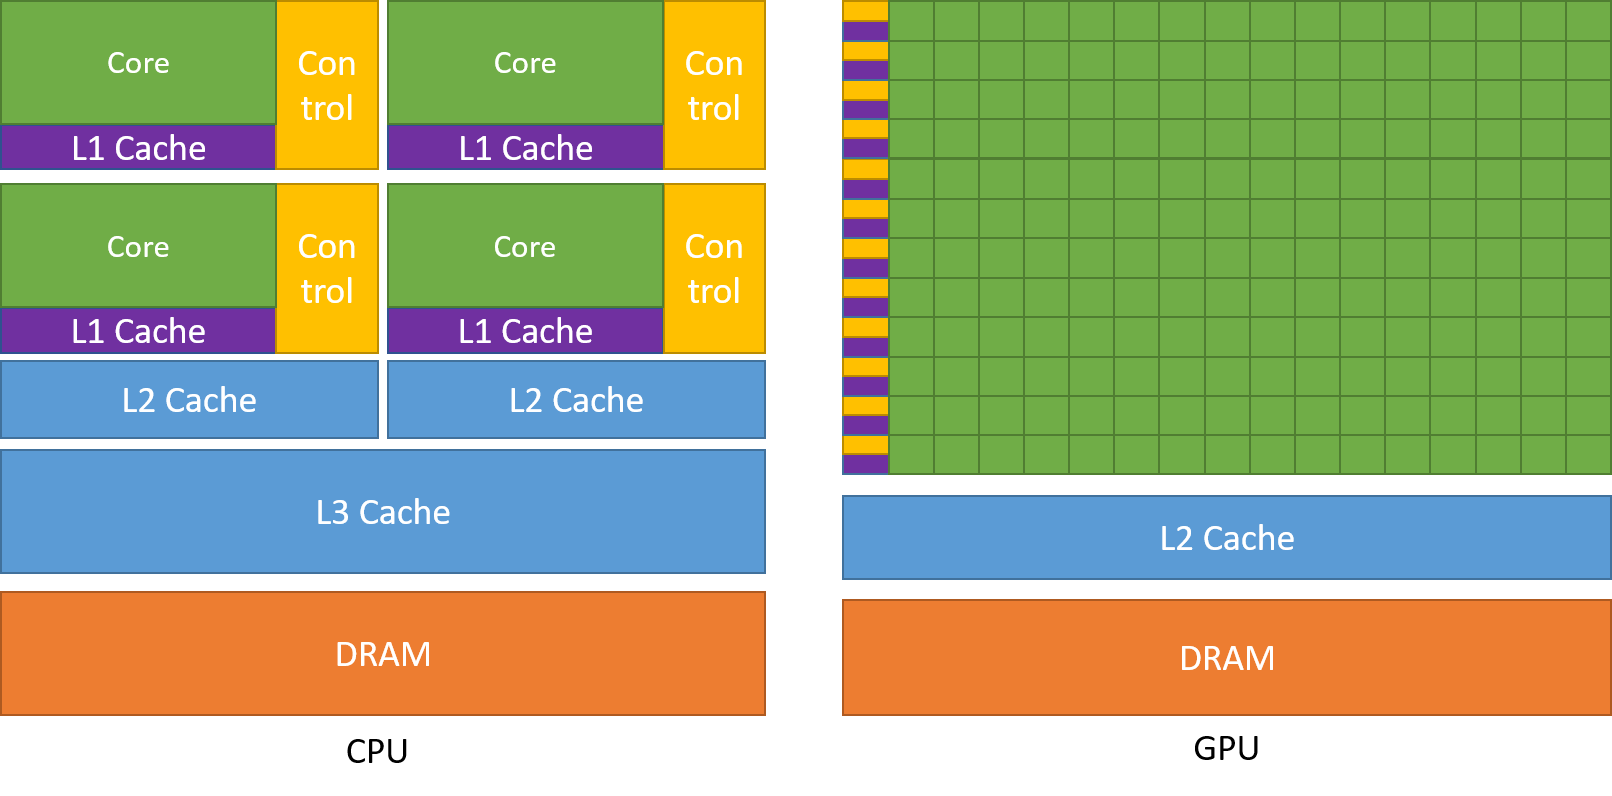
\includegraphics[width=0.8\linewidth]{Images/gpu-devotes-more-transistors-to-data-processing.png}
    \caption[GPU vs CPU transistor allocation for data processing.]{The GPU devotes 
more transistors to data processing than the CPU. Each (green) core acts as a thread 
that executes the same instruction on different data elements. Source: 
\cite{nvidia2025cuda}.}
    \label{fig:gpu-architecture}
\end{figure}        

A GPU executes a large number of lightweight threads (Figure 
\ref{fig:gpu-architecture}), organised into warps, groups of 32 threads that execute 
the same instruction simultaneously on a single streaming multiprocessor (SM). This 
single-instruction multiple-thread (SIMT) model maps directly onto operations such as 
FFTs, element-wise multiplication, and threshold comparisons, where the same 
computation is applied independently to many data elements. When threads within a warp 
follow different control flow paths — a condition known as warp divergence — the 
divergent branches must be executed serially, reducing parallelism (see Figure 
\ref{fig:warp-diverge}).

\begin{figure}
    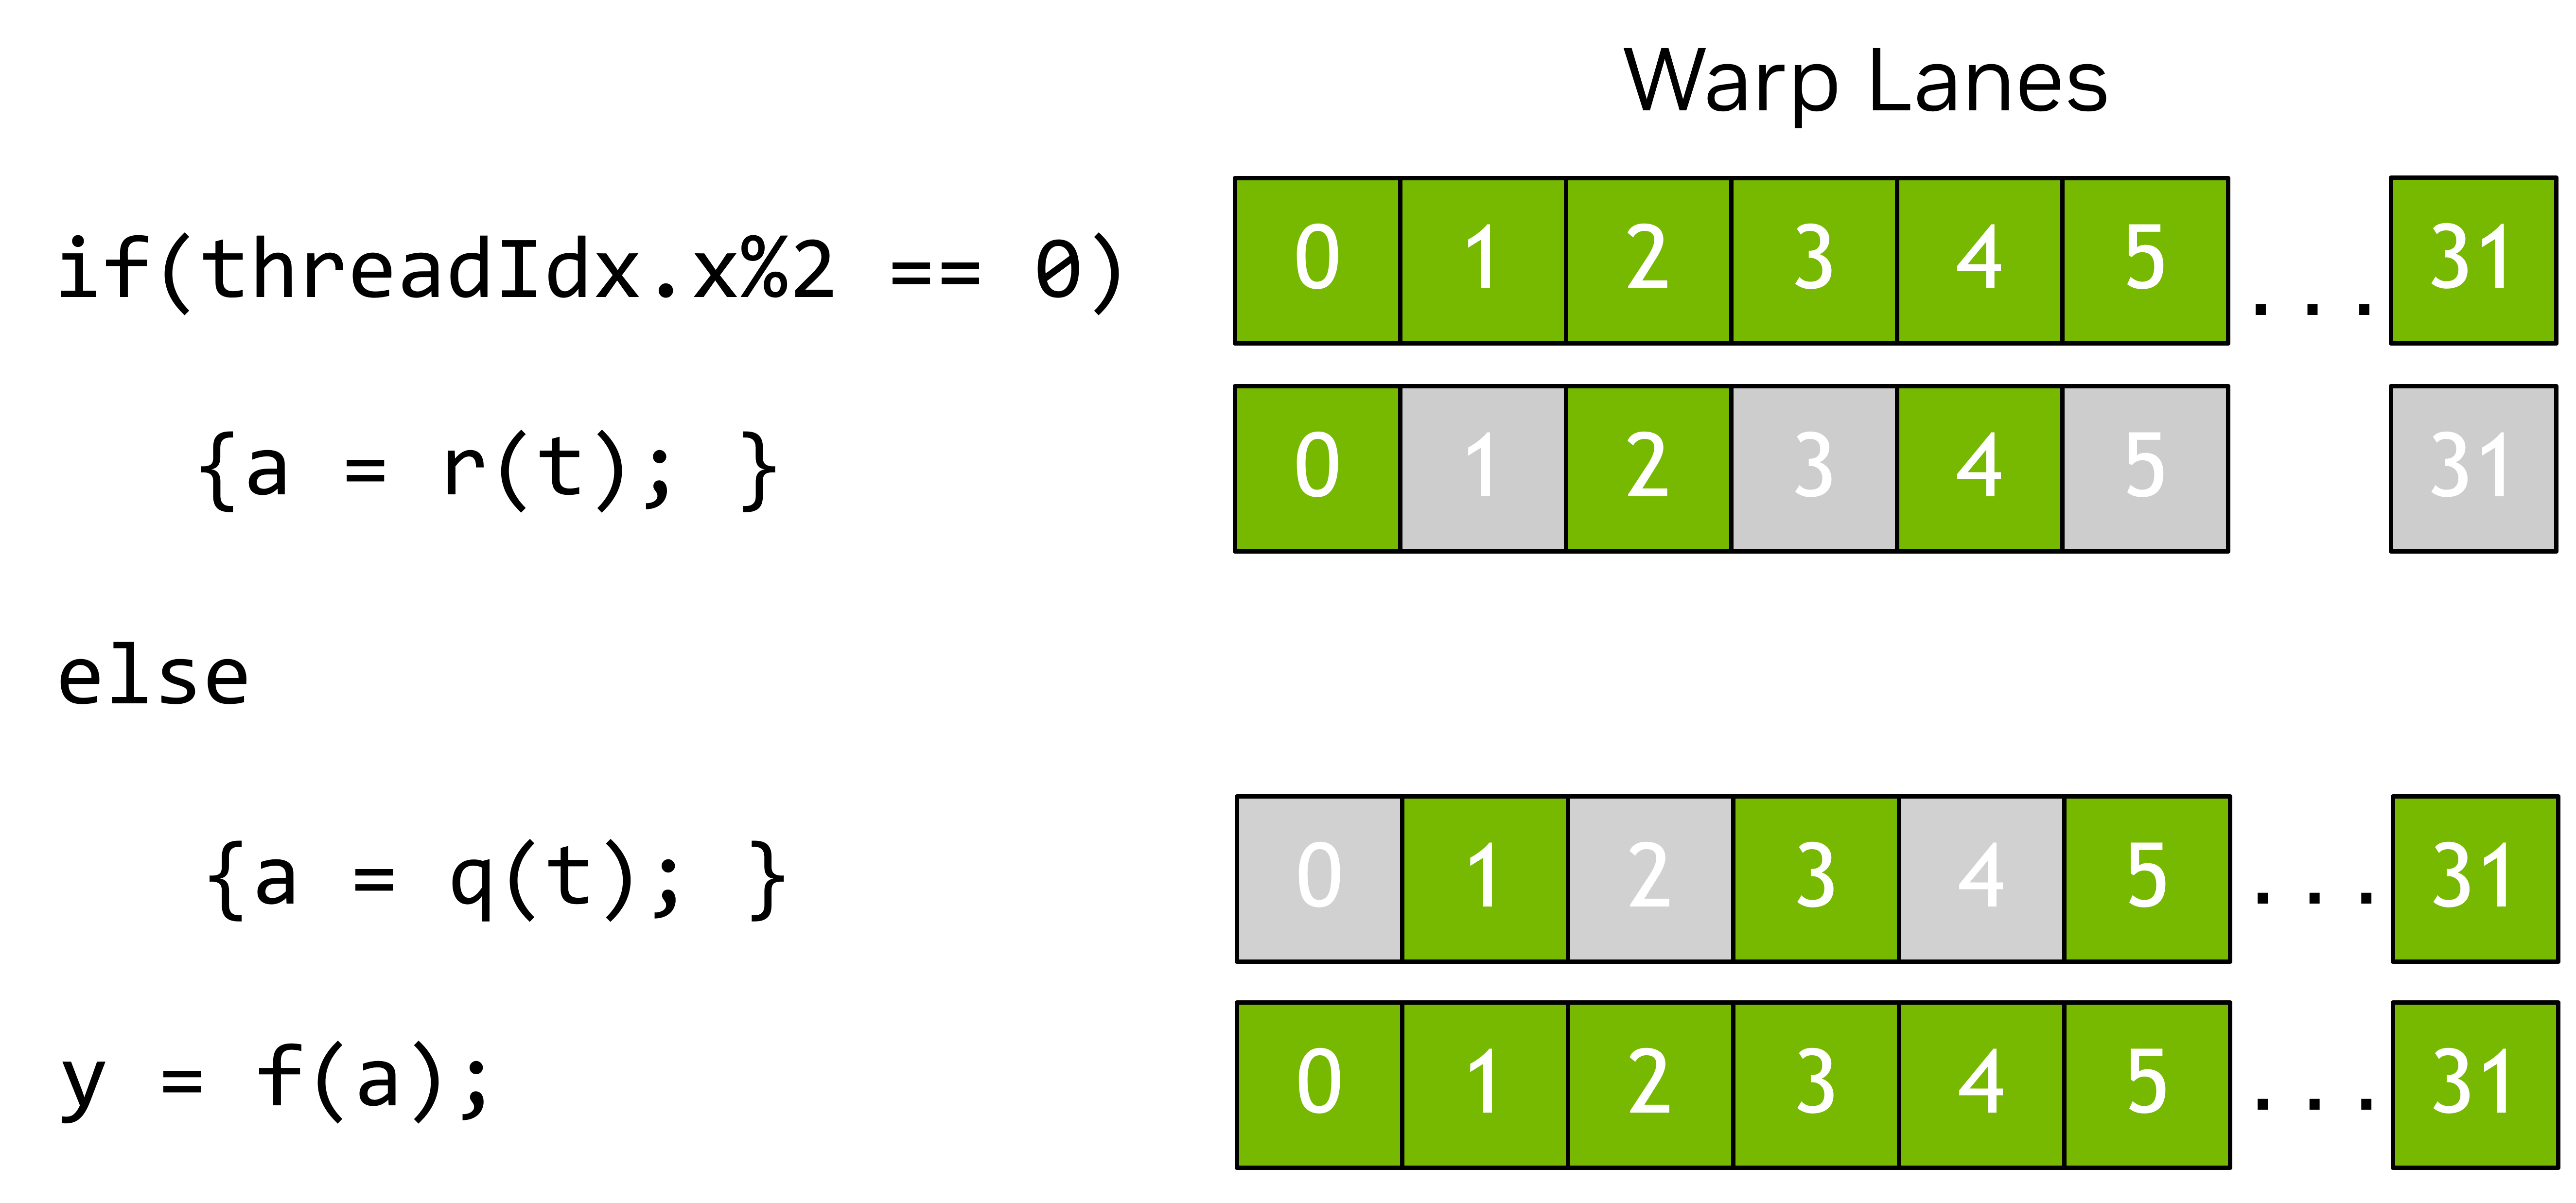
\includegraphics[width=0.8\linewidth]{Images/active-warp-lanes.png}
    \caption[Warp divergence causing serial execution of divergent branches.]{In this example, branching
    paths in execution between the even and odd threads prevent all threads from executing in parallel.
    All even threads execute the top branch while all odd threads are idle, then vice versa. As a result,
    the execution time is the sum of the two branches instead of the maximum. 
    Source: \cite{nvidia2025cuda}.}
    \label{fig:warp-diverge}
\end{figure}

Memory access patterns also affect throughput. Global memory is accessed most 
efficiently when threads in a warp read or write contiguous memory locations 
simultaneously, a pattern known as coalesced access. Non-coalesced access wastes
memory bandwidth by reading non-contiguous memory locations.
Figure \ref{fig:coalesced-access} illustrates one such situation. The warps will need 
to retrieve data from global memory more frequently when accessing non-contiguous 
memory. For this reason, ensuring that as much as possible of the data in each cache 
line fetched is actually used is an important part of performance optimisation of 
memory accesses on these devices.

\begin{figure}
    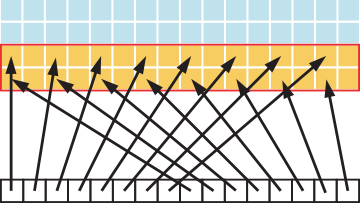
\includegraphics[width=0.5\linewidth]{Images/adjacent-threads-accessing-memory-with-stride-of-2.png}
    \caption[Non-coalesced memory access with stride of 2 reducing bandwidth efficiency.]{Figure 6:
    Adjacent threads (bottom) accessing every second memory location (orange). Since memory is cached in 
    large blocks,
    the large stride of 2 results in a 50\% reduction in load/store efficiency, since half of all cached
    memory is not being used. Source: \cite{nvidia2025cuda}.}
    \label{fig:coalesced-access}
\end{figure}

In discrete GPU systems, the CPU and GPU maintain separate physical memory pools 
connected by a bus such as PCIe, and data must be explicitly transferred between host 
and device memory. In system-on-chip (SoC) platforms such as the NVIDIA Jetson family, 
the CPU and GPU share the same physical DRAM. This is called physically shared memory. 
Both processors access the same physical addresses, and the memory subsystem handles 
coherency, eliminating the explicit transfer step.

Shared memory is a separate, small, low-latency scratchpad memory local to each SM, 
explicitly managed by the programmer. It allows threads within a thread block to 
exchange data and cache intermediate results without accessing global memory. It is 
used in GPU implementations of reductions, transpose operations, and tiled matrix 
multiplications, where threads cooperatively load a tile of data into shared memory and 
reuse it across multiple operations.
\chapter{Literature Review}
\label{ch:literature_review}
% \input{Sections/Ch3 Literature Review/Low SWaP Aerial Radar.tex}
% \input{Sections/Ch3 Literature Review/GPU radar processing performance.tex}
% \input{Sections/Ch3 Literature Review/Low SNR Monopulse feasability.tex}
% \input{Sections/Ch3 Literature Review/Programmable Vision Acceleration for Radar.tex}
% \input{Sections/Ch3 Literature Review/Summary.tex}

\section{Compact Airborne Radar for UAV DAA}
% Try to emphasise that there are not field trials that validate a full 
% target tracking pipeline under realistic encounter conditions
The work of Sysak et al.\ 
\cite{sysak2025_lightweight_compact_pulse_radar_uav_collision_avoidance}, 
Wang et al.\ \cite{Wang2016}, and Moses et al.\ \cite{6044363, Moses2015}
each tackle important subproblems in the design of a radar DAA system for 
small UAVs, but each leave important gaps unaddressed in the literature. 

Sysak et al.\ 
\cite{sysak2025_lightweight_compact_pulse_radar_uav_collision_avoidance} 
present a lightweight X-band monopulse radar for mid-air collision avoidance 
on medium UAV platforms, integrating a multi-channel forward-looking antenna 
with FPGA-based pulse compression on a single 60 gram PCB, with average power 
below 80 Watts. Field trials demonstrate reliable detection of large obstacles 
at 1--3 km (see Figure \ref{fig:sysak}), as well as detection of a 3.15 m 
wingspan UAV from 6.4 km. The work 
validates a simple online pipeline from range compression to \gls{tcpa} estimation,
but does not characterise the pipeline's latency or tracking performance, nor 
explain if the detections were make during sensing, or post-processed from recorded data. 

\begin{figure}
    \incfig[0.9]{sysak_radar}
    \caption{Sysak et al.'s experimental set up and results. The radar is 
    capable of detecting large targets at 1--3 km with high ranging accuracy. 
    We observe peaks in amplitude over range that correspond to target position.}
    \label{fig:sysak}
\end{figure}

Moses et al.\ \cite{6044363} in a 2013 publication introduces a 230 gram 
miniature radar mountable 
on a small quadcopter (see Figure \ref{fig:moses-quadcopter}), to demonstrate the feasibility of integrating radar
sensing onto very small platforms. Their evaluation emphasises target 
identification via 
micro-Doppler signatures rather than ranging or tracking, achieving a 100\% 
detection rate when 7 meters away from the target. When distance increased
and both the platform and target took to the air, accuracy dropped significantly.
This difference in performance between ground-based and airborne targets highlights
the importance of validating radar pipelines under realistic encounter conditions. 
While the work provides a dataflow diagram for the processing pipeline, it does not
characterise the latency of the stages not compare alternative algorithmic choices. 
Lastly, while the work discusses the difficultly of radar under SWaP-C constraints, 
the final weight, size, and power consumption of the radar system are not reported.

A follow up 2014 publication by the same group (Moses et al.\ \cite{Moses2015})  
presents an even smaller radar (see Figure \ref{fig:moses-2014}) with angle sensing 
capabilities and collision avoidance
algorithms, in attempt to further demonstrate more capabilities of miniature radar 
with respect to UAVs DAA systems. In this work, the radar is only evaluated indoors with large reflective 
targets. While the collision avoidance algorithms are compared thoroughly, no other
algorithm choices are evaluated and readiness for open air tests was not demonstrated.
For example, the authors note that a higher transmit power is needed. 

\begin{figure}[htbp]
    \centering
    \begin{minipage}{0.4\textwidth}
        \centering
        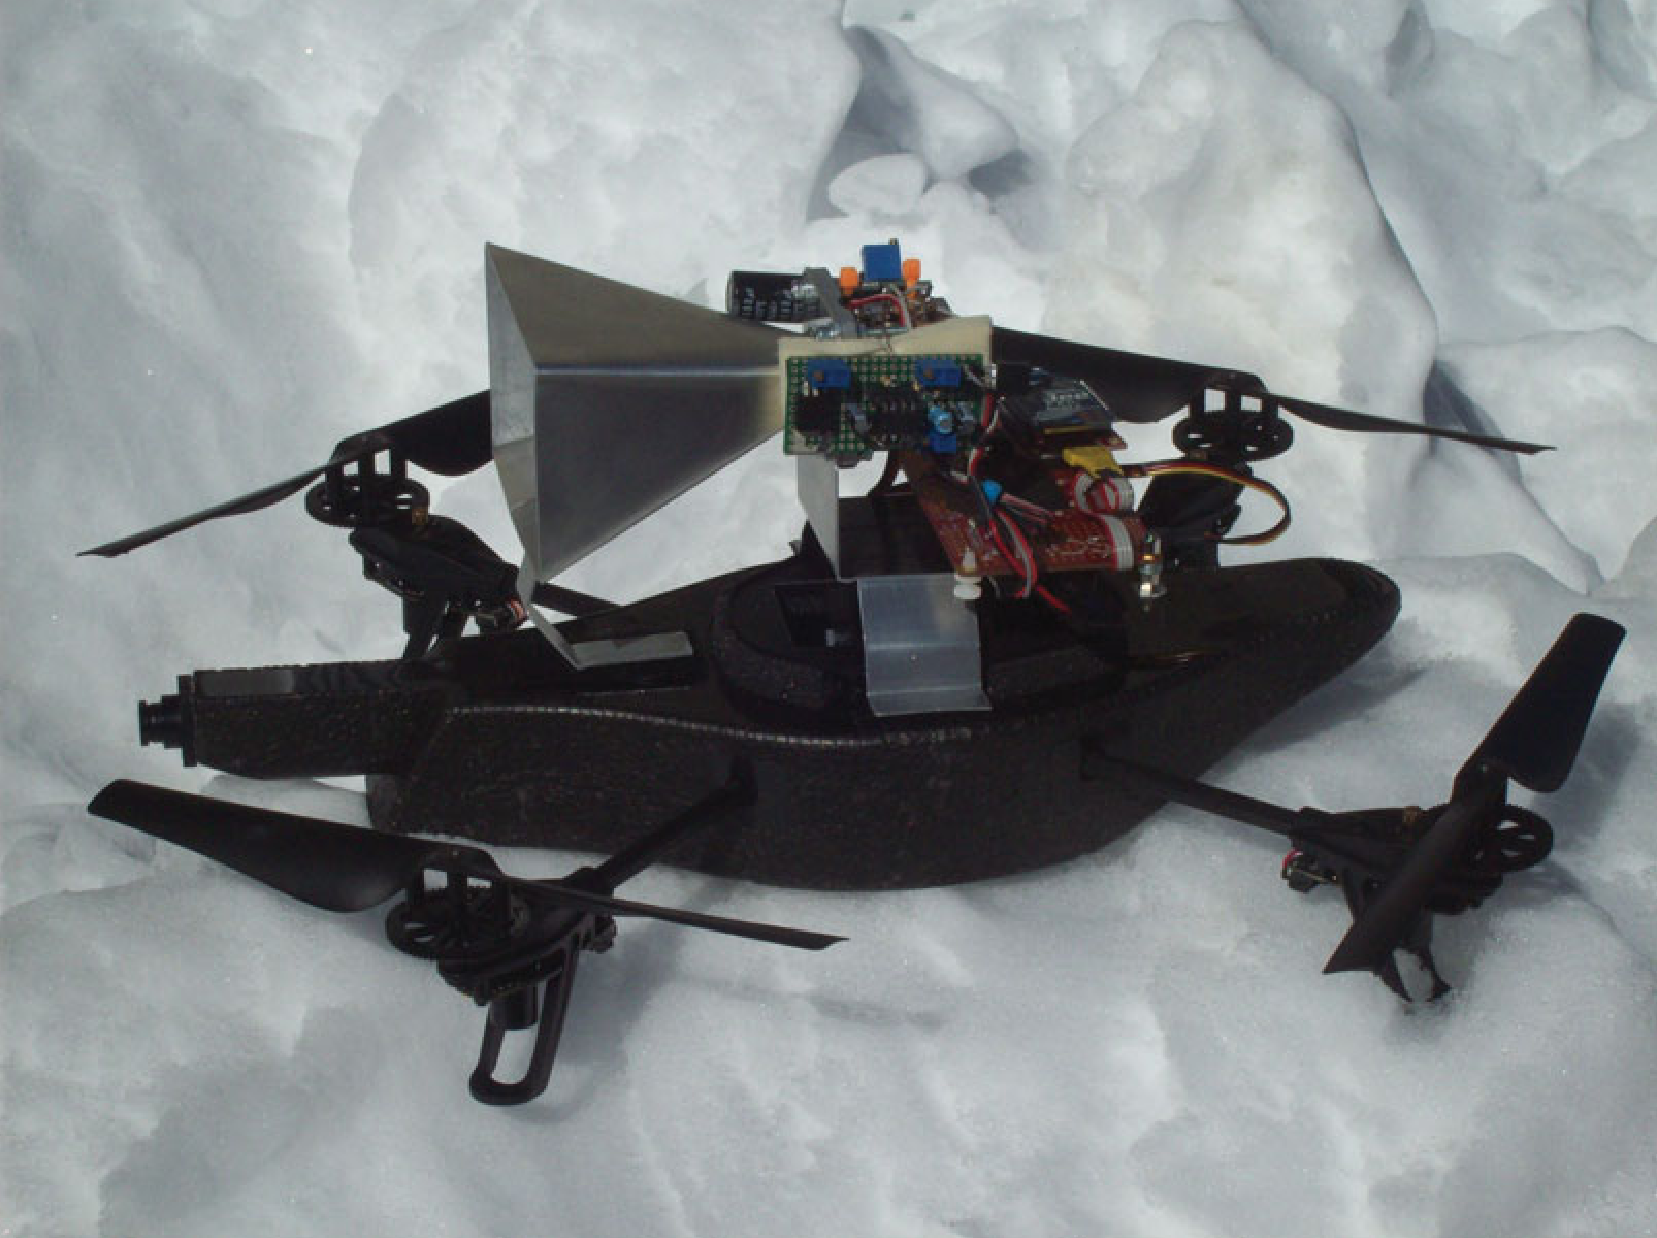
\includegraphics[width=\linewidth]{Moses 2013 quad copter.png}
        \caption{Moses et al.'s miniature radar mounted on a small quadcopter.}
        \label{fig:moses-quadcopter}
    \end{minipage}
    \begin{minipage}{0.4\textwidth}
        \centering
        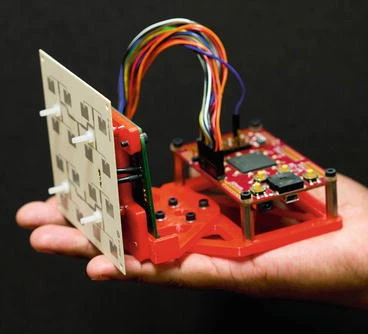
\includegraphics[width=\linewidth]{moses-2014.png}
        \caption{Second Generation of Moses et al.'s miniature radar, now
     with angle sensing capabilities.}
        \label{fig:moses-2014}
    \end{minipage}
\end{figure}

% Cool work that does ranging with big and small targets with light radar
% Pretty low-key research that just does some maths
% 
Wang et al.\ \cite{Wang2016} demonstrate a complete low-SWaP LFMCW system 
design for group 2/3 UAS (10-600 kg) group 2/3 UAS incorporating FFT-based 
detection, digital beamforming, and GPU-accelerated FFT for update rate 
improvement. The research highlights the feasibility of measuring the range
of targets 5+ km away through beamforming, but angle sensing capabilities were 
not explored. Additionally, design performance is validated in simulation only, 
and does not take into account compute and latency constraints. 
This thesis addresses these gaps by providing hardware-validated latency and 
throughput measurements for a comparable pipeline, and by substantiating the 
choice to use the GPU for certain operations with systematic benchmarks.

While research such as that of Mohammad Karimi et al. \cite{Mohammadkarimi2024} 
does support the feasibility of electronically scanning to measurement 
azimuth and elevation of targets, this work also does not characterise the
system in a realistic encounter scenario, only validating ranging and
angle estimation in simulation. While the work is rigorous in its mathematical
treatment of \gls{daa} requirements, empirical validation of the software
pipeline is needed to show that such a system can operate under the SWaP constraints
of a small \gls{uav}. 

Angle sensing, an important capability for UAV DAA, is not addressed
in Sysak et al.\ \cite{sysak2025_lightweight_compact_pulse_radar_uav_collision_avoidance},
Wang et al.\ \cite{Wang2016}, or Moses et al.\ \cite{6044363} \cite{Moses2015}, and is 
presented but not validated in Mohammad et al.\ \cite{Mohammadkarimi2024}. 

This thesis addresses these gaps by characterising the software pipeline by latency and
track quality, placing an emphasis on angle sensing, and by comparing the performance
of alternative algorithmic choices.  

This thesis addresses the gaps in Moses et al.'s work by evaluating the radar 
pipeline on real radar hardware data from open-air long-range scenarios, and 
by systematically comparing alternative algorithmic choices for each stage of 
the software pipeline, including FFT, integration, CFAR, monopulse angle sensing
and multi-target tracking under the SNR conditions characteristic of 
small-aperture UAV radars.

This thesis addresses the lack of empirically validated radar target tracking
pipelines by implementing a complete software pipeline and evaluating it and
comparing generated tracks to ground truth tracks. Additionally, attention will
be paid towards the ability for the pipeline to run in real time on board a small
\gls{uav}. 

\section{GPU-based Radar Processing Under SWaP Constraints}
The work of Shi et al.\ \cite{6712628}, Newmeyer et al.\ \cite{7577322}, 
Zhao et al.\ \cite{rs15225421}, and Zaknoun 
\cite{zaknoun2024_realtime_gpu_accelerated_radar_processing} 
each explore the computational challenges of small airborne radar systems
across different contexts. Still important gaps remain unaddressed across 
all literature.

Shi et al.\ \cite{6712628} describe a small \gls{fmcw} phased array built from 
off-the-shelf development boards, validating that continuous real-time 2D FFTs 
are achievable on a 100 MHz FPGA. However, processing was split between an 
onboard FPGA and offboard post-processing, and signal coherence problems 
prevented real-world validation. This thesis addresses this gap by implementing 
a fully onboard, online pipeline and validating it against real target returns.

Newmeyer et al.\ \cite{7577322} demonstrated a 120 gram, 8 Watt \gls{fmcw} phased 
array pipeline on a Zynq ARM CPU, closely monitoring power, latency 
distributions, and hardware resources. This work clearly establishes that 
radar DAA can operate under strict SWaP constraints. However, only one 
hardware configuration and one algorithm sequence are evaluated. This thesis 
addresses this gap by systematically comparing alternative algorithmic 
pathways and evaluating how pipeline bottlenecks change across embedded 
compute configurations, including GPU-based architectures.

Zhao et al.\ \cite{rs15225421} implement CUDA acceleration for a passive 
bistatic radar pipeline, reporting up to a 113.13$\times$ speedup over a CPU 
baseline across three algorithm stages. However, the study covers only clutter 
suppression, range--Doppler processing, and CA-CFAR detection, omitting angle 
estimation, coordinate transforms, and Kalman filtering, and does not discuss 
memory reallocation or thread synchronisation costs. This thesis addresses 
these gaps by benchmarking a more comprehensive algorithm selection and 
profiling host--device transfer and synchronisation overhead explicitly.

Zaknoun \cite{zaknoun2024_realtime_gpu_accelerated_radar_processing} provides 
a comprehensive treatment of GPU radar software architecture for real-time 
processing. However, this work is not situated in a UAV DAA context and does 
not evaluate performance under UAV SWaP constraints. This thesis adapts these 
architectural insights to the UAV DAA problem, evaluating how conclusions 
change under constrained power and memory budgets.

\section{Sensitivity and Detection in Low-SNR Regimes}

A key consequence of SWaP-constrained hardware is reduced aperture, which 
simultaneously lowers SNR and degrades angular resolution, increasing the 
likelihood that multiple targets occupy the same resolution cell.

An et al.\ 
\cite{an2024_time_varying_angle_estimation_unresolved_extended_targets_monopulse} 
propose an efficient method for resolving two unresolved targets within a 
single monopulse cell. However, evaluation is limited to simulated white-noise 
conditions, the method is not integrated into an end-to-end range--Doppler 
pipeline, and explicit failure modes exist for same-angle targets and 
cells containing three or more targets. This thesis addresses these gaps by 
testing the algorithm under non-white noise conditions and within a complete 
tracking pipeline, measuring the effect on track quality.

Aubry et al.\ 
\cite{aubry2020_single_pulse_simultaneous_detection_angle_estimation_multichannel} 
demonstrate that detection and angle estimation can be treated jointly in a 
multichannel array, increasing sensitivity to targets not visible in any single 
channel and avoiding the brittleness of early thresholding under low SNR. 
However, validation is limited to single simulated targets in Gaussian 
interference. This thesis addresses this gap by applying the algorithm to 
multiple targets under non-Gaussian noise regimes and measuring both 
sensitivity and track-quality impacts alongside compute cost.

The noise and clutter regime experienced by a miniature airborne radar has not been empirically
characterised in the literature. Ezuma et al.\ \cite{ezuma2019microuav} demonstrate that
Gaussian and Rayleigh clutter assumptions — the basis of CA-CFAR — already fail for
ground-based mmWave radar detecting UAVs, finding that a Weibull distribution provides a
significantly better fit to the measured clutter statistics, and explicitly noting that prior
UAV detection work had neglected this. The airborne case, where the radar sensor is itself
mounted on a vibrating UAV platform subject to altitude variation, aspect angle changes, and
platform-induced interference, introduces further departures from the homogeneous Gaussian
noise model that underpins standard windowing and CFAR algorithm selection. No published work
has measured or modelled these statistics for a miniature airborne FMCW radar in real flight
conditions. As a result, the algorithm choices made in existing pipeline designs, (window
function selection, CFAR variant, and training cell configuration) lack empirical
justification for this operating regime.

\section{Summary and Research Gap}
Across the UAV DAA radar literature three gaps emerge. First, existing 
hardware demonstrations validate detection against large, high radar 
cross-section targets only; no work characterises sensitivity to small 
moving airborne targets under realistic encounter conditions. Second, 
processing feasibility on constrained embedded hardware has been demonstrated 
on FPGAs and ARM CPUs, but no work benchmarks a GPU-based pipeline in a UAV 
DAA context with comprehensive algorithm coverage and architectural profiling. 
Third, the noise and clutter regime of miniature airborne FMCW radar has not been empirically
characterised. Existing work shows that Gaussian clutter assumptions fail even for ground-based
mmWave radar, yet no study has measured these statistics for an airborne sensor. As a result,
the window function, CFAR variant, and training cell choices made in existing pipeline designs
lack empirical justification for this operating regime, and angle sensing algorithms have only
been validated under idealised white Gaussian noise with single simulated targets.

This thesis addresses all three gaps by characterising detection and tracking
sensitivity against small moving airborne targets, by benchmarking a
comprehensive selection of radar processing and tracking algorithms on embedded
GPU hardware with explicit profiling of host--device transfer and
synchronisation overhead, and by collecting real flight data to characterise the
noise regime and evaluate monopulse angle sensing algorithms within a complete
multi-target tracking pipeline under realistic conditions.
\chapter{Methodology}
\label{sec:methodology}
% \todo{Describe the design of our experiment. Break down experiment into sub experiments, how does that relate to the different subsystem we are building.}
% \todo{Describe the tools and processes we will use to validate our software. Nsight systems, nsight compute, other tools for measuring memory. Bash scripts for testing}
\section{Overview}
This thesis designs, implements, and evaluates a software-defined radar processing 
pipeline for a small monopulse radar system, assessing both computational efficiency 
and tracking accuracy on an NVIDIA Jetson Xavier NX and a Xavier AGX embedded GPU platform. 
The methodology is structured to directly address the gaps identified in the literature review: the
absence of radar algorithm performance evaluation in the noise regimes of air-to-air
small aperture radar, low level
implementation analysis, and hardware-aware design conclusions under SWaP constraints.
Through the methodology outlined in this chapter, we fulfill the contributions of this 
thesis, to compare radar algorithm configurations by sensitivity and track quality, to compare
low-level implementations by computational performance, and to derive hardware-aware design 
recommendations.

The software processing pipeline is designed to receive the radar data from multiple 
Texas Instruments 
AWR2243 radar chips, and produce tracks of targets in the radar's field of view. For 
the experiments performed in this work, we utilise data from a conformal synthetic 
aperture radar. Both the radar hardware and the software are designed to be modular. 
The radar module, depicted in Figure \ref{fig:radar-module},
has up to 12 receiver patches that are arranged in a 6x2 grid, conforming to a curved surface.
For testability, the software system is broken up into three subsystems, which are in turn 
comprised of stages that each perform a specific radar processing function. 
The three subsystems are: a pre-processing subsystem which is concerned with preparing 
the raw radar data for detection, an aggregator subsystem, which is concerned with combining the 
processed data from multiple video streams into a single stream, and a detection and tracking 
subsystem, which is concerned with detecting targets in the radar data and tracking them over time. 
This subsystem level design is depicted in Figure \ref{fig:system-level-dataflow}. 

\begin{figure}
    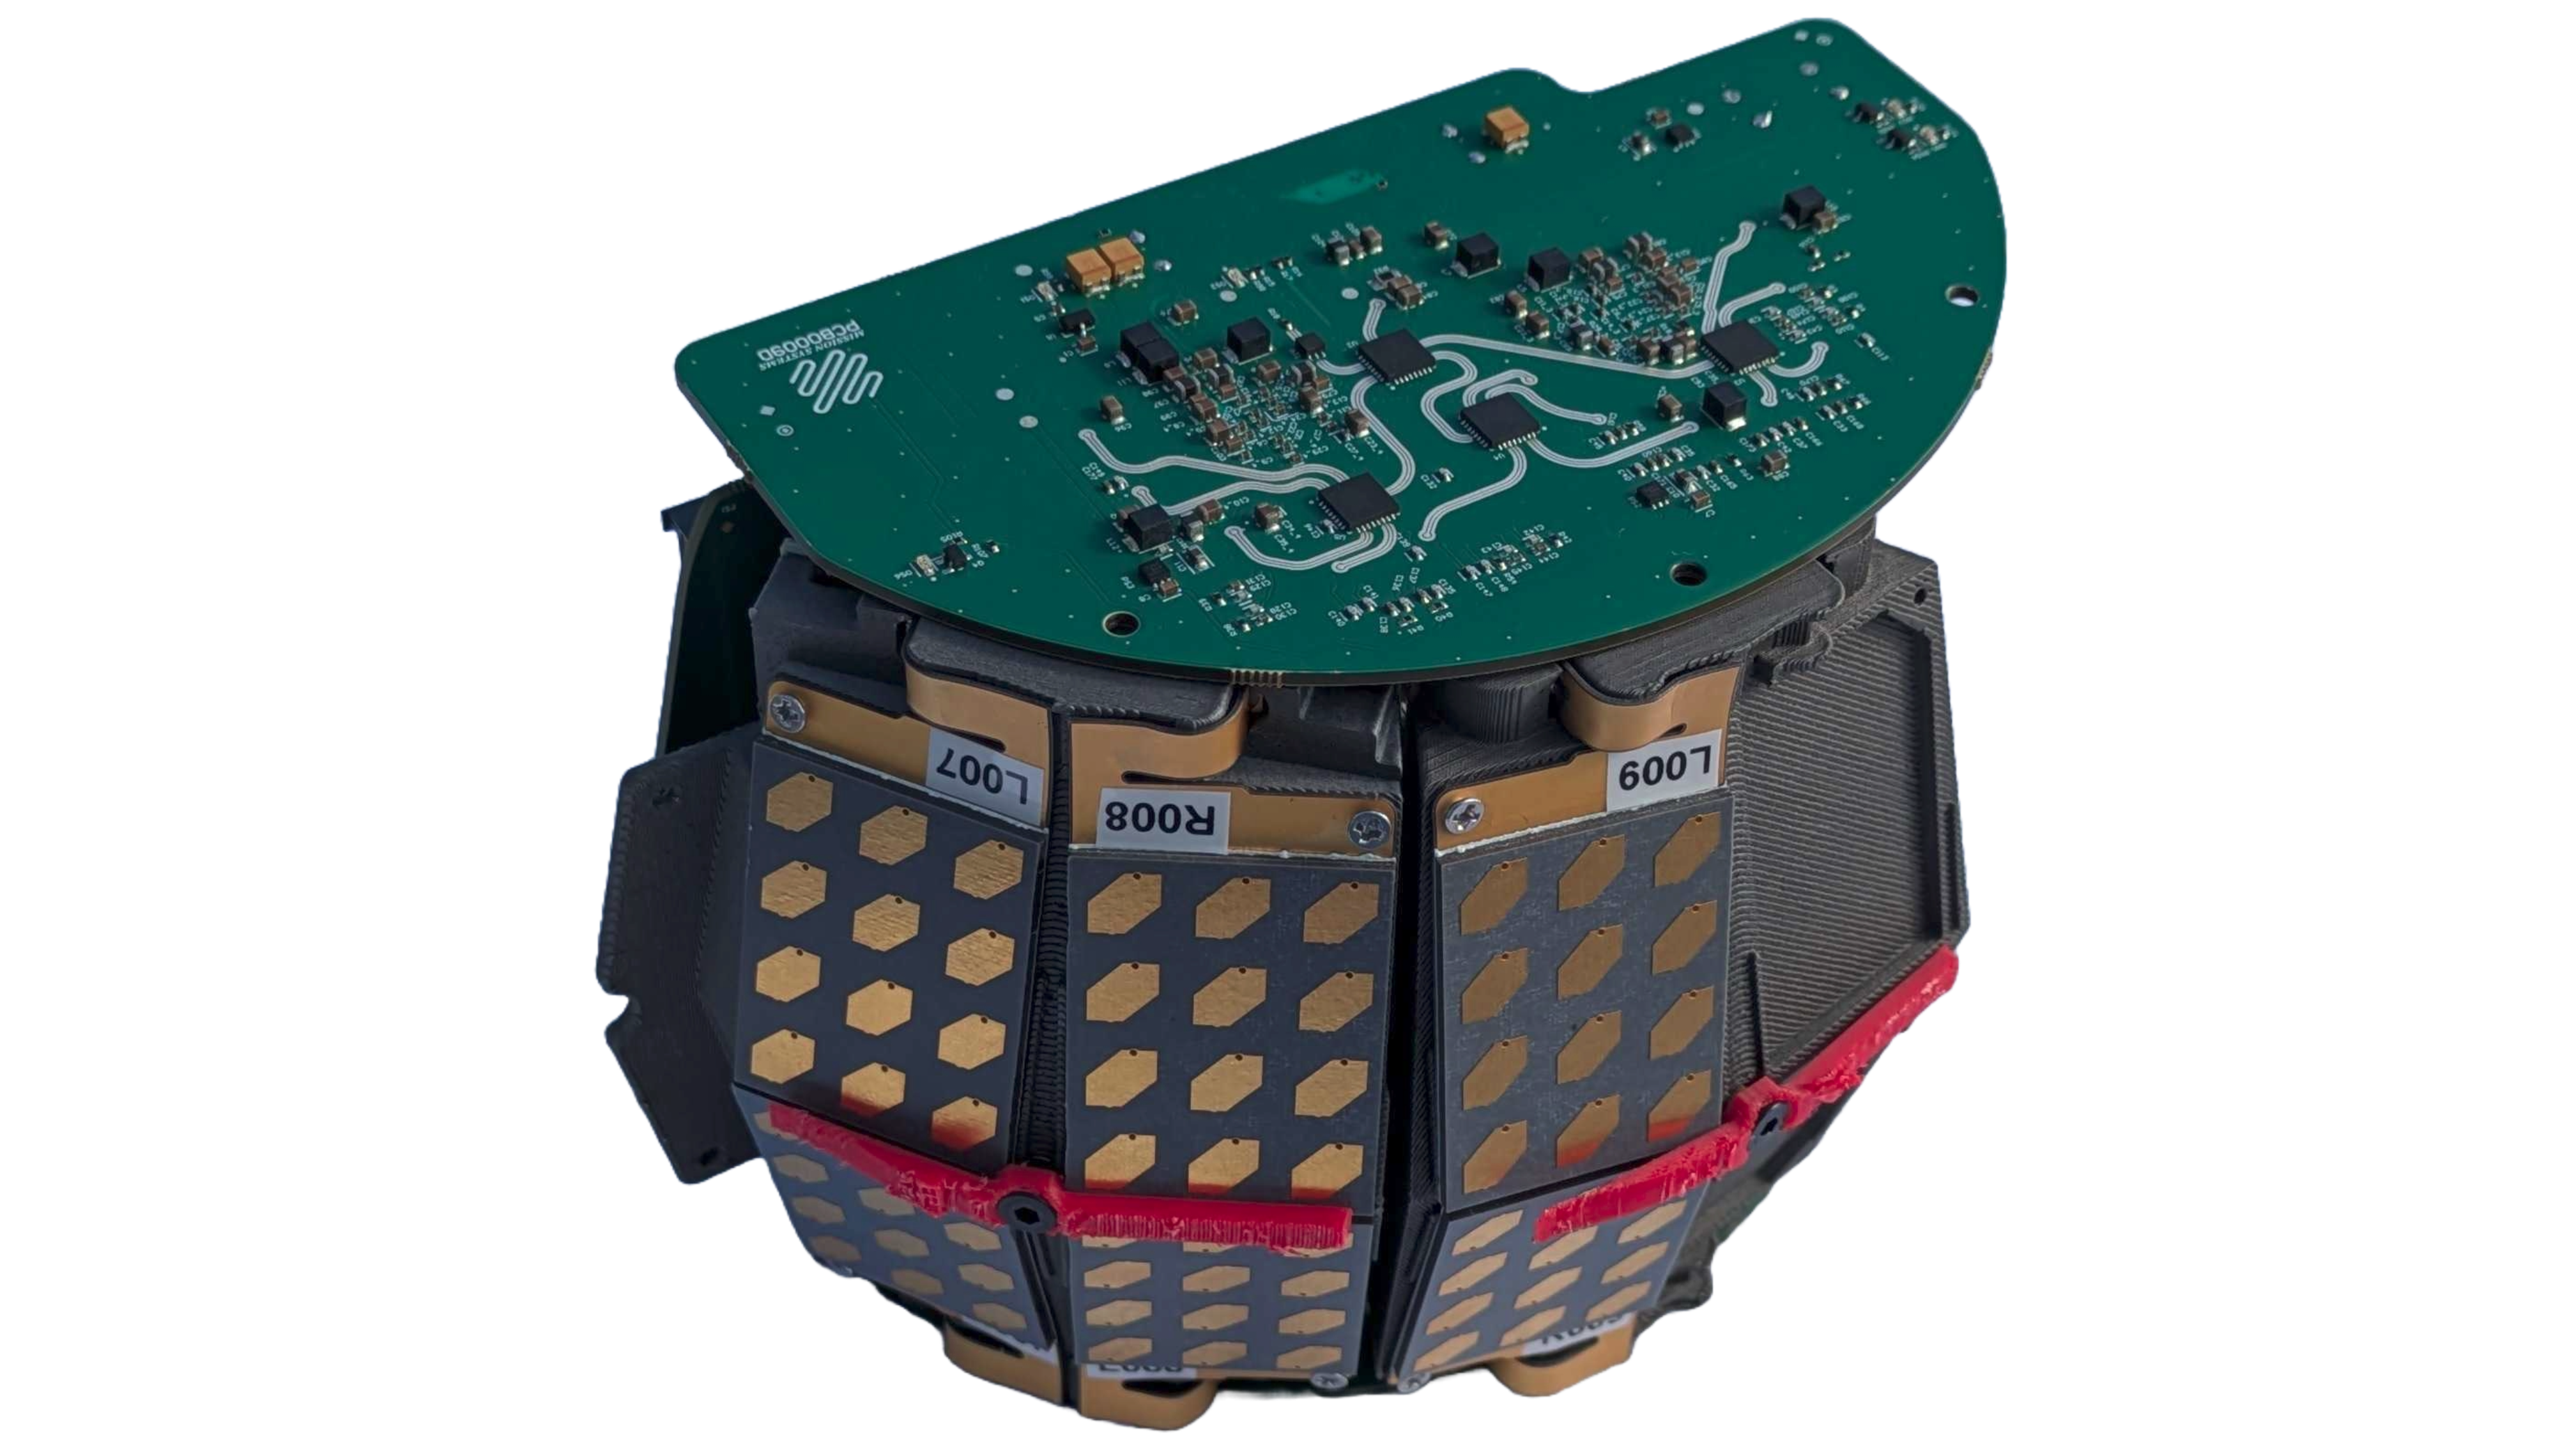
\includegraphics[width=0.7\textwidth]{radar_module.png}
    \caption[Radar Module Photo]{Photo of the radar module with its 6 of its 12 receiver 
    patches arranged in a 3x2 grid.}
    \label{fig:radar-module}
\end{figure}

\begin{figure}[htbp]
    \centering
    \incfig[0.9]{application_level_dataflow} 
    \caption[\small System-level dataflow diagram of the radar pipeline.]{\small System level dataflow diagram. The pre-processing subsystem receives the AWR2243's raw
    radar data over four CSI video streams. The data is organised into frames, each containing many
    chirps. The processing subsystem then outputs
    the data in the form of chirps containing target range information. The aggregator subsystem
    receives the four resulting processed data streams, and combines them into a single data stream
    organised by quadruplets, a collection of four receivers necessary for monopulse angle sensing.
    The detection and tracking subsystem receives a stream of quadruplet chirps, and produces tracks of
    targets in the radar's field of view.}
    \label{fig:system-level-dataflow}
\end{figure}

The methodology is organised into three parts. Firstly, we propose a design of a \mbox{(pre-)processing} 
subsystem that performs formatting, windowing, FFTs, and coherent integration on dense radar data. 
Then, we propose the design of a detection and tracking subsystem that performs CFAR, monopulse angle 
sensing, clustering, and multi-target tracking. Lastly, we describe the datasets used for testing.

\FloatBarrier
\section{Processing Subsystem Evaluation}
\label{sec:processing_app}
The proposed preprocessing subsystem is responsible for receiving the raw radar data from the AWR2242 
radar chips, depicted in Figure \ref{fig:AWR2243},
and preparing the data for detection. An instance of the subsystem runs per incoming video stream. 
Before outputting the data to the aggregator subsystem which is upstream of the detection and 
tracking subsystem. The subsystem performs the following operations sequentially: formatting, windowing, FFT, and 
integration, (see Figure \ref{fig:preprocessing-dataflow}). Below are the implementation and 
experiment details for each of the operations. 

\begin{figure}[htbp]
    \centering
    \incfig[1]{preprocessing_dataflow} 
    \caption[Dataflow for the preprocessing subsystem.]{Dataflow for the preprocessing subsystem. Multiple instances of the subsystem run on
    separate processes, with each instance receiving compressed baseband radar data samples from an
    incoming video stream. Formatting organises samples into contiguous blocks in memory, and discards
    empty chirps. The windowing stage applies a window function to the data to reduce spectral smearing
    in the next stage. The \gls{fft} stage applies a Fourier Transform across fast time into the frequency
    domain, revealing target range. The coherent integration stage sums the complex \gls{fft} values of
    identical pulses within the same frame.} 
    \label{fig:preprocessing-dataflow}
\end{figure}

\begin{figure}
    \centering
    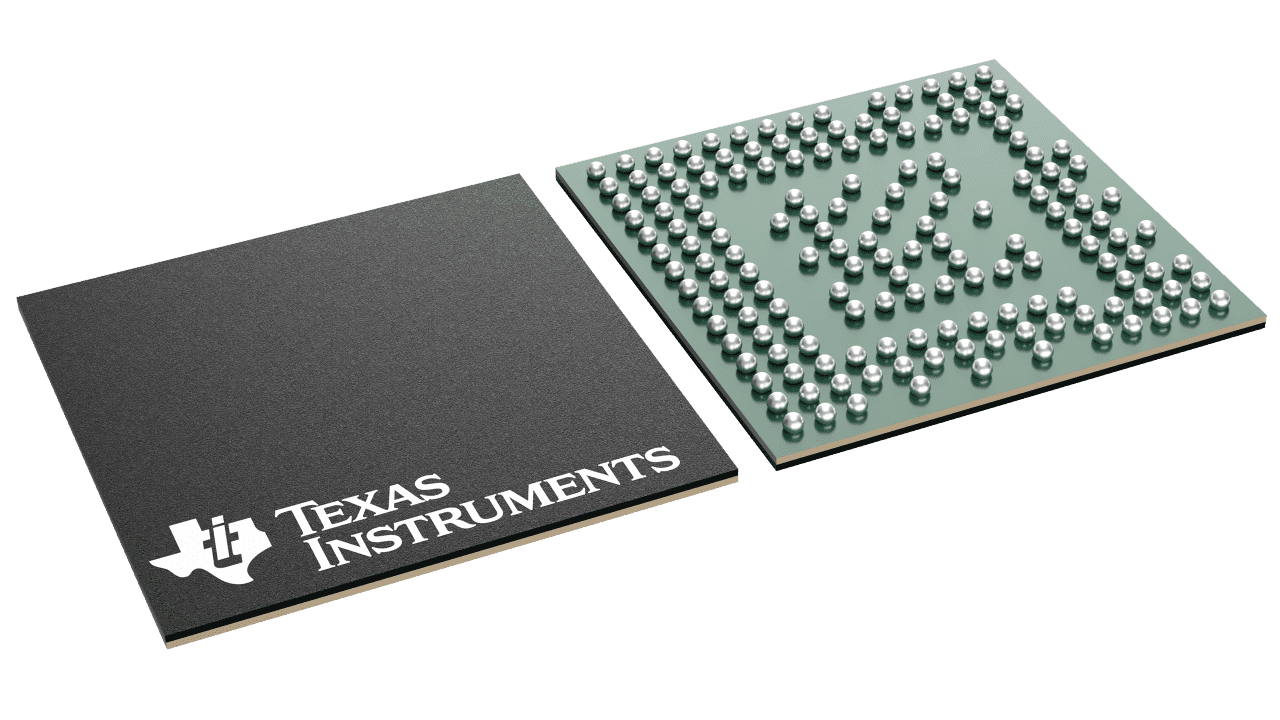
\includegraphics[width=0.5\textwidth]{AWR2243.png}
    \caption[Texas Instruments AWR2243 radar chip.]{Photo of the Texas Instruments AWR2243 radar chip, which is
    used in the radar module. The chip has 3 transmitters and 4 receivers, and outputs the radar data over a CSI
    video stream. The chip is only 10.4mm x 10.4mm, making it suitable for placement on UAV PCBs.}
    \label{fig:AWR2243}
\end{figure}

\subsection{Windowing}
To reveal target range from a single radar pulse, an \gls{fft} is applied to the
de-chirped pulse. 
% The  assumes the finite signal repeats periodically, so when the signal does
% not start and end at the same value, the implicit periodicity introduces a discontinuity. This
% causes energy from a true frequency to spread into adjacent bins — a phenomenon known as spectral
% leakage.

When an \gls{fft} is performed on a finite signal, it is implicitly multiplied by a rectangular window.
A term-wise multiplication in time corresponds to a convolution in the frequency domain, and the
rectangular window's sinc-shaped frequency response has large sidelobes that spread energy from
each frequency bin into its neighbours. By applying a more suitable window function prior to the
FFT, spectral leakage can be reduced, as shown in Figure \ref{fig:hann filter}.

\begin{figure}[htbp]
    \centering
    \includesvg[width=0.6\linewidth]{Images/ffts1}
    \caption[FFT with and without a Hann window showing spectral leakage reduction.]{Results of an \gls{fft} performed on a signal with two frequencies and Gaussian noise, with
    and without a Hann window. Without the Hann window, the bins close to the peak frequency bins 40
    and 45 are significantly elevated due to spectral leakage from those peaks, which would cause
    nearby bins to be falsely detected as targets.}
    \label{fig:hann filter}
\end{figure}

This thesis evaluates a range of practical window functions and their implementation on CPU and GPU. 
Candidate windows include common real-time tapers such as Hann and Hamming, lower-sidelobe windows 
such as Blackman and Blackman--Harris, and adjustable-parameter windows such as Kaiser, which allow 
explicit control over sidelobe level and mainlobe width. Because windowing is a point-wise 
multiplication, it is naturally suited to single instruction, multiple data (SIMD) execution. These 
implementations are compared for their resulting spectral behaviour. 

The sidelobe attenuation and resolution loss are compared for each window and a trade off analysis 
is performed to determine when each window is the most suitable. These procedures provide a basis 
for selecting windows that are spectrally well behaved, sensitive, and 
positively affect the ending track quality. 

\subsection{Integration}
Coherent integration is compared with non coherent integration for their resulting SNR 
improvement, angle estimation quality, and track quality on real and simulated data. 
The relationship between coherent integration window size and the performance metrics 
is also explored. 

After, the latency and throughput of coherent integration is characterised in relation to
the other stages, and the integration window size. The trade off analysis is 
between SNR and latency is performed. The integration stage is also evaluated in the
ablation study of the processing application. 
\section{Detection and Tracking Application Evaluation}
\label{sec:tracking_app}
The proposed detection and tracking subsystem is responsible for receiving the processed 
radar data
across all radar channels from the aggregator subsystem, and producing tracks of
targets in the radar's field of view. The subsystem performs the following operations
sequentially (see Figure \ref{fig:dat-dataflow}): CFAR, clustering, monopulse 
angle sensing, sidelobe suppression (blanking), and multi-target tracking.
Below are the implementation and experiment details for each of the operations.

\begin{figure}[H]
    \centering
    \incfig[1]{detection_and_tracking_dataflow} 
    \caption[Dataflow diagram for the detection and tracking subsystem.]{Dataflow for the detection 
    and tracking subsystem. The subsystem receives the processed radar data across all radar 
    channels from the aggregator subsystem, and produces tracks of targets in the radar's 
    field of view. The subsystem performs the following operations sequentially: CFAR, clustering, 
    monopulse angle sensing, sidelobe suppression (blanking), and multi-target tracking.}
    \label{fig:dat-dataflow}
\end{figure}

\subsection{CFAR}
For finding the CFAR coefficient $\alpha$ (defined in \ref{eqn:threshold}) that gives a desired false 
alarm rate $P_{fa}^{\star}$. The relationship between these variables (Equation 
\ref{eqn:cfar_false_alarm}), cannot be rearranged into a closed-form expression. 

\begin{equation}
    P_{fa}(\alpha;N) = \left( \frac{N}{N+\alpha} \right)^N
    \sum_{k=0}^{3} \binom{N+k-1}{k}
    \left( \frac{\alpha}{N+\alpha} \right)^k
\end{equation}

Since $P_{fa}(\alpha;N)$ is strictly decreasing in $\alpha$, bisection can be used 
to find the value of $\alpha$ that gives the desired false alarm rate \(P_{fa}^{\star}\).

The method begins with $\alpha_{lo}=0$ and increases an upper bound $\alpha_{hi}$ until 
$P_{fa}(\alpha_{hi};N) \leq P_{fa}^{\star}$. It then repeatedly bisects the interval and evaluates 
$P_{fa}(\alpha;N)$ at the midpoint, updating the lower or upper bound depending on whether the resulting 
false alarm rate is above or below the target. This continues until the interval is sufficiently small. 
In this way, $\alpha$ is obtained as the numerical solution that gives the required false alarm rate.

Additionally, three different implementations of CFAR are compared for their latency: a naive
implementation on the CPU, an implementation that uses a prefix sum table, and a naive solution on the
GPU. Additionally, different noise assumptions are tested. The naive implementation involves calculating 
the noise statistic with a repeated sum per sample of interest (see Figure \ref{fig:naive-cfar}). 
The prefix sum table method reduces the 
number of sums required to four per sample of interest regardless of the number of training cells, the
start and end of the left and right window (see 
Figure \ref{fig:prefix-sum-table}). The GPU implementation creates a thread per sample of interest (see 
Figure \ref{fig:gpu-cfar}). A sweep of window size, guard size, frame buffer size and false alarm rate values is 
conducted for each CFAR implementation on real and simulated data. The performance (throughput, latency, 
false alarm rate, sensitivity, and track quality) is compared across configurations in a cost benefit 
analysis. 
This addresses the literature gap in understanding how detection sensitivity and false alarm behaviour 
trade off against latency and throughput under SWaP constraints.

\begin{figure}[!ht]
    \incfig[0.75]{cfar}
    \caption[Naive CPU CFAR implementation.]{Naive Implementation of CFAR for the CPU. Each sample is compared to a threshold
    determined by the power of the samples around it. The threshold is calculated by taking the
    average power of the surrounding samples and multiplying it by a factor \(\alpha\) determined
    by the desired false alarm rate.}
    \label{fig:naive-cfar}
\end{figure}

\begin{figure}[htbp]
    \incfig[0.75]{prefix_sum_table}
    \label{fig:prefix-sum-table}
    \caption[CFAR using a prefix sum table for constant-time noise statistics.]{CFAR implementation using a prefix sum table (cumulative signal power). The prefix sum
    table allows the noise statistic to be calculated with a fixed number of sums per sample of
    interest, regardless of the number of training cells. In this specific case, after the cumulative
    signal power is calculated in processing, it only takes four sums of to find the sum of eight
    training cells.}
\end{figure}

\begin{figure}[htbp]
    \incfig[0.75]{gpu_cfar}
    \label{fig:gpu-cfar}
    \caption[Parallel GPU CFAR implementation.]{CFAR implementation on the GPU. Threads (each depicted as unique colours) are each
    responsible for a sample, allowing for parallel processing of the CFAR algorithm across the entire
    range profile. Each thread calculates its own noise statistic, threshold, and mask.}
\end{figure}

The literature gap regarding algorithmic selection is addressed through an exploration of different CFAR
algorithms, including OS-CFAR, CA-CFAR, SO-CFAR, and GO-CFAR. The effect of these algorithms on detection
sensitivity and track quality is compared. For intuition, Figure \ref{fig:cfar-algorithms} illustrates
the difference in performance of the algorithms on a synthetic signal with 5 peaks. This work 
compares the performance of GO-CFAR, SO-CFAR, and CA-CFAR on simulated data and discusses
the downstream effects of this selection, addressing the literature gap regarding the impact of 
detection algorithms in the noise regimes of miniature radar. Additionally, by analysing the 
performance of both CPU and GPU implementations of CFAR, the literature gap regarding the 
algorithmic implementation under SWaP constraints is addressed. 

\begin{figure}
    \centering
    \incfig[0.81]{cfar_stacked_matched_colours}
    \caption{ Performance of four CFAR variants. Each 
    algorithm registers a detection when its threshold is 
    below the signal. The test signal has 5 peaks that are 
    each surrounded by different noisy distributions. The bottom 
    plot illustrates the detections made by each algorithm. 
    OS-CFAR performs well in this example.}
    \label{fig:cfar-algorithms}
\end{figure}

\subsection{Clustering}
After CFAR occurs, most of the samples (range bins) will be zero. The efficiency loss from 
processing so many zero samples motivates a stage that transforms the detection sparse 
representation into a dense one. Additionally, the widening of the main lobe of each of 
the detections due to the windowing stage creates multiple range bins with detections 
from the same target, which motivates a stage that groups these samples into a single 
detection.
The algorithm that addresses both of these problems, clustering, iterates through the 
range profile, and creates a cluster for each contiguous set of 
detection samples. Then, the complex signals from each of the samples are summed together. 
SNR is expected to improve, as noise will be incoherent within clusters, but the signal
that corresponds to a target will have the same phase across samples, and thus will be 
coherent. The latency of both CPU and GPU implementations of the clustering algorithm 
is measured. Different clustering parameters are tested for their impact on tracking performance, such 
as the allowed gap size between detections.

\subsection{Monopulse Angle Sensing}
Angle sensing converts multi-channel detections into azimuth, elevation and range estimates that 
drive association and tracking. We assess candidate angle discriminators by running controlled 
sweeps over SNR, channel 
imbalance, and multi-target proximity, and measuring angular bias, mean squared error, and confidence. 
The latency and throughput of CPU and GPU implementations are measured. The trade-off involves software implementation details such as warp divergence and instruction-level parallelism. 

The angle sensing algorithm features a few early returns that result in warp divergence on the GPU. 
For example, if the bearing and elevation ratios are outside of the domain over which the polynomial
fit is valid. Instruction level parallelism is a measure of how many instructions can be executed 
in parallel on a single thread. By changing the order of operations, we can potentially increase instruction-level parallelism and reduce the latency of the GPU implementation.

\subsection{Sidelobe Suppression (Blanking)}
When a target exists outside of the field of view of a given radar receiver, the receiver may still
register a detection due to the sidelobes of the antenna pattern. When a target is in the radar's 
field of view, it will land in the main lobe of some receivers and the sidelobes of others (see Figure 
\ref{fig:sidelobes}), resulting
in a strong detection in the correct direction and weaker detections in the wrong directions, all at
the same range. The blanking stage eliminates detections that are likely to be sidelobes by eliminating
detections that are close in range to a stronger detection at the same time step. 

\begin{figure}[htbp]
    \centering
    \begin{minipage}{0.5\textwidth}
        \centering
        \incfig[1]{sidelobes}
        \caption[Sidelobes of the antenna pattern.]{Receivers R1 and R3, which are pointing away from the target,
        still receive significant power from the first sidelobes lining up with the target. }
        \label{fig:sidelobes}
    \end{minipage}
    \begin{minipage}{0.45\textwidth}
        \centering
        \incfig[1]{blanking}
        \caption[Blanking for sidelobe suppression.]{Detections from the sidelobes of R1 and R3 are weaker 
        than R2's detection from the main lobe, and are close in range to R2's detection. R1 and R3's
        detections that are close in range to a stronger detection at the same time step are eliminated.}
        \label{fig:blanking}
    \end{minipage}
\end{figure}

\begin{figure}[htbp]
\end{figure}

The blanking stage will be implemented on the CPU. After clustering and angle sensing, 
the detections come in an ordered list per receiver quadruplet. A CPU implementation would involve,
for each time step, iterating through each of the lists simultaneously and sorting them into one ordered list in O(N) 
time. Then iterating through the ordered list and eliminating detections that are close in range to
a stronger detection. 

% GPU DETAILS BELOW, POTENTIALLY USEFUL
% A GPU implementation would involve creating a thread per detection per quadruplet, 
% performing 3 binary searches to figure out how many detections are nearer than it in range to the radar,
% and mapping itself to the corresponding place in the fully sorted list. In a second pass then, each 
% thread would check the detections near it in the fully sorted list to see if there are any stronger
% detections in range. Since this problem is a standard k-way merge sort, the CUDA Thrust library 
% implementation will be used. This stage can also double as a receiver fusion stage, as detections
% from multiple receivers across different chirps that are close in not just range but also angular 
% position can be merged 
% together. 

\subsection{Multi-Target Tracking}

\begin{figure}[htbp]
    \centering
    \incfig[1]{tracking_dataflow} 
    \caption[Dataflow diagram for the tracking subsystem.]{Dataflow for the tracking stage of the 
    detection and tracking subsystem. Detections are fed into the
    associator of the multi-target tracker, and are then fed into the hypothesiser. 
    The hypothesiser produces a hypothesis per track/detection pair. The associator then 
    finds the optimal assignment
    of detections to tracks. The updater then updates the tracks, and the deleter deletes 
    tracks with poor quality. For the detections that are not associated with any tracks,
    a tentative track is initiated or updated in the initiator, a miniature tracker that
    handles the track initiation and confirmation process. 
    }
    \label{fig:tracking-dataflow}
\end{figure}

The multi-target tracking stage will be implemented entirely on the CPU due to its sequential nature. 
Amplitude based association will be compared to non-amplitude based association for their impact on
track quality. The multi-target tracker has over 20 parameters that can be tuned, and one 
configuration of these parameters will be validated and discussed. Experiments will
be conducted in a variation of SNR, and number of targets, in simulated data. Real 
data will be used to validate the results on static targets. The literature gap regarding the impact
of algorithmic choices in the tracking stage on track quality is addressed through this experiment. 

% EXPLORE MORE
% - Non amplitude based association
% - Amplitude based association
% - ringing 

% \section{Testing Datasets}
% The datasets described below are used for the experiments outlined in the following sections (see Sections \ref{sec:processing_app}, and \ref{sec:tracking_app})
% \begin{itemize}
%     \item \textbf{Generic Sine Waves with Noise}: To validate the correctness of our processing 
%     algorithms as well as their speed, we generate binary files of synthetic radar data consisting of 
%     a complex sine wave with additive white Gaussian noise. This allows us to test the software under 
%     controlled conditions where we can precompute the expected output, and to evaluate the performance 
%     of the software in terms of latency and throughput without the confounding factors of real-world 
%     data. (INCLUDE FIGURE HERE illustrating the signal)  
%     \item \textbf{AWR2243 Recorded Data}: To validate the operation of our pipeline with realistic 
%     data speeds, timing uncertainties, and electrical noise, we record data from our AWR2243 radar 
%     system in TEST\_SOURCE mode. In test source mode, two targets can be simulated on the chip with 
%     position velocity and bounds. The receivers record what the reflected signals from these targets 
%     would look like. While the data recorded is not fully representative of real-world data, it allows 
%     us to test the software with realistic data rates and noise characteristics. 
% \end{itemize}

\section{Testing Datasets}
The datasets described below are used for the experiments outlined in the previous sections 
(\ref{sec:processing_app} and \ref{sec:tracking_app}).

The first dataset is used 
to validate both the correctness and the speed of our processing algorithms during development. 
By generating binary data streams containing complex sine waves with Gaussian noise using bash scripts, 
we can test the radar software under controlled conditions where the expected output can be precomputed 
in advance. This makes it possible to verify algorithmic correctness while also evaluating latency and 
throughput without the additional complexity introduced by real-world phenomena such as multipath 
propagation, data corruption, and non-gaussian noise. An interactive variation of this dataset is 
also used for debugging, allowing the user to adjust parameters such as SNR, range, and bearing/elevation
ratios in real. Figure \ref{fig:synthetic-signal} illustrates an example of a synthetic signal generated 
for testing.

\begin{figure}
    \incfig[0.6]{dataaset1}
    \caption[Example of a synthetic signal generated for testing.]{An 
    example of a synthetic signal generated for testing. The top plot shows the real components of the 
    samples of many received chirps (stacked vertically). Fast time increases to the right and the height 
    of a sample within a chirp is its voltage. In the bottom plot, the horizontal axis is now range, 
    successive chirps are stacked vertically and amplitude is depicted with colour, where yellow is the highest 
    amplitude. 2nd plot is produced by applying an \gls{fft} to each synthetic chirp from the first plot. 
    The transform allow us to visually validate that the frequency to range conversion is correct, 
    and the preprocessing stage is behaving as expected.}
    \label{fig:synthetic-signal}
\end{figure}

The second dataset consists of recorded data from the AWR2243 radar system operating in \verb|TEST_SOURCE| 
mode. This dataset is used to validate the behaviour of the processing pipeline under more realistic 
data rates, timing uncertainties, and electrical noise conditions. In \verb|TEST_SOURCE| mode, the chip can 
simulate two targets with configurable position, velocity, and bounds, and the receivers capture the 
signals that would be reflected from these targets. Although this recorded data is still not fully 
representative of real-world radar returns, it provides a more realistic approximation of practical 
operating conditions than the synthetic sine wave dataset. 

\chapter{Results}
\section{Overview}
This chapter presents the validation process and results of the processes outlined in the 
Methodology (Chapter 
\ref{sec:methodology}). The results are organised by operation. Each section
discusses the correctness and computational performance of an algorithm. Additionally implementation 
decisions for each of the stages are compared for both their speed and accuracy. The results are 
presented as plots, and are accompanied by a discussion of their implications for the design 
of the radar processing pipeline in the following chapter. 

Before the per stage performance is presented, a holistic view of the pipeline's performance is
given, including the ablation study on each of the hardware devices and field trial results.  

The pipeline demonstrates full real-time multi-target tracking functionality on each of the three
hardware platforms: the desktop workstation, the NVIDIA Xavier 
AGX, and the NVIDIA Xavier NX. Best case, the desktop workstation 
can run the whole pipeline at 100 frames per second when the maximum integration size is used, 
the Xavier AGX and NX performed at 500 and 400 frames per second in the same case.  

On top of this, the harness used for visualisation can also run online, 
allowing the user to see the correct 
behaviour of each of the stages of the pipeline in real time. Examples of these visualisations are
for each of these stages are depicted in Appendix Figures  \ref{fig:fft-visual}, 
\ref{fig:cfar-visual}, \ref{fig:cluster-visual}, \ref{fig:angle-visual}, \ref{fig:track-visual1}, 
and \ref{fig:track-visual2}. These figures have been included as a reference for how to visualise
and validate the intermediate stages of a radar processing pipeline. Understanding these 
visualisations is also important for interpreting 
the following figures in this section: \ref{fig:integration-waterfall}, 
\ref{fig:integration-waterfall-orac}, \ref{fig:integration-setup}, \ref{fig:cfar-0.001-waterfall},
\ref{fig:clustering-results}, \ref{fig:angle-2d-plot}, \ref{fig:angle-3d-plot-noise},
\ref{fig:tracking-scenarios}, \ref{fig:tracking-3d-results}.

% Filenames: visual-fft-png, visual-angle.png, visual-cfar.png, visual-cluster.png, visual-track.png
\subsection{Pipeline Ablation Study}

Throughout this chapter, the \emph{integration size} $N$ is the number of
consecutive input chirps that are coherently summed to produce a single output
chirp (record). Equivalently, it is the factor by which the chirp count is
reduced by the integration stage: an integration size of $N$ maps $N$ input
chirps to $1$ output chirp, so the two descriptions --- the number of
summations and the factor of reduction --- refer to the same quantity. Thus an
integration size of $1$ applies no reduction ($256$ output chirps for $256$
input chirps), while the maximum integration size of $256$ applies the greatest
reduction ($1$ output chirp for $256$ input chirps). Larger integration sizes
therefore produce less output data per frame and are the least demanding case
for downstream throughput.

An ablation study is performed on each of the devices 
to determine the contribution of
each stage to the overall latency of the pipeline and their
marginal effects on its throughput. Latency is measured as 
the time between the arrival of a chirp to the capture stage of
the processing subsystem, and the
generation of the output of the pipeline, whatever it may be. 
Throughput is measured as the number of frames processed per 
second after processing 1000 frames each of 52.5 MB in size. 
Dataset DS2 simulates the 
receiver signals of targets across a wide variety of ranges in
high noise. On each trial, the complete pipeline is run up until 
a given terminating stage, for example, label "CFAR" refers to the 
pipeline including all stages up to and including CFAR. 

On the desktop, performance requirements were easily met, and 
a frame rate of above 100 frames per seconds was achieved for the maximum integration 
size of 256, that is 1 output chirp (record) for every 256 input chirps 
(see Figure \ref{fig:ablation-throughput-desktop}). 
One optimisation that was significant was the use of several CPU threads to handle the incoming
frames. Utilising two or four processing buffers allowed the pipeline to maintain 15+ framerate 
even when the integration stage didn't compress the data at all (an integration size of 1, i.e. 
256 output chirps per 256 input chirps). 
Another finding 
made on the desktop was that after CFAR, additional stages only marginally reduced throughput, 
suggesting that host-device transfer, and CPU read/write operations dominated the pipeline's 
compute time. 

On the two Jetson Devices, the device-host memory architecture disallows the asynchronous 
graph execution that was possible on the desktop, limiting CPU operations to one thread. 
The Jetson devices performed with higher performance than the desktop workstation, achieving 
framerates of 25-500 and 20-400 frames per second on the AGX and NX respectively depending on 
integration size (see Figure 
\ref{fig:latency-jetsons}) the latency chart for the desktop workstation and the throughput 
diagrams of the Jetson devices (which will just show the reciprocals of the latencies) is in the 
Appendix \ref{fig:latency-desktop} \ref{fig:throughput-nx} \ref{fig:throughput-agx}.

\begin{figure}
    \centering
    \incfig[0.8]{ablation_throughput_desktop}
    \caption{Pipeline framerate, for 
    different integration sizes (the number of input chirps summed per output 
    chirp, equivalently the factor of reduction). 
    Obtained by finding average frames 
    per second after processing 1000 frames of 52.5 MB each. Each line shows 
    the framerates of the pipeline running up to a given stage. The largest reductions 
    in framerate occur at the integration stage, aggregation stage, and CFAR stage. Frame 
    rate varies from 16 to 100 for the entire pipeline depending on the integration size.}
    \label{fig:ablation-throughput-desktop}
\end{figure}

\begin{figure}
    \centering
    \incfig[0.9]{Ablation_Latency_Breakdown_Jetsons}
    \caption{Pipeline latency breakdown as stages are added for 
    different integration sizes (the number of input chirps summed per output 
    chirp, equivalently the factor of reduction). 
    Split into the processing subsystem
    the detection and tracking subsystem, 
    and a combined view. The capture, integration, aggregation, CFAR and tracking stages 
    are the most significant }
    \label{fig:latency-jetsons}
\end{figure}

\subsection{Tracking Performance at Field Trials}
The radar hardware was taken to an open air field test site in New South Wales 
where it and a target drone were flown in a variety of scenarios. Figure 
\ref{fig:real-world-tracking} depicts one such air to air scenario. 
\begin{figure}
    \centering
    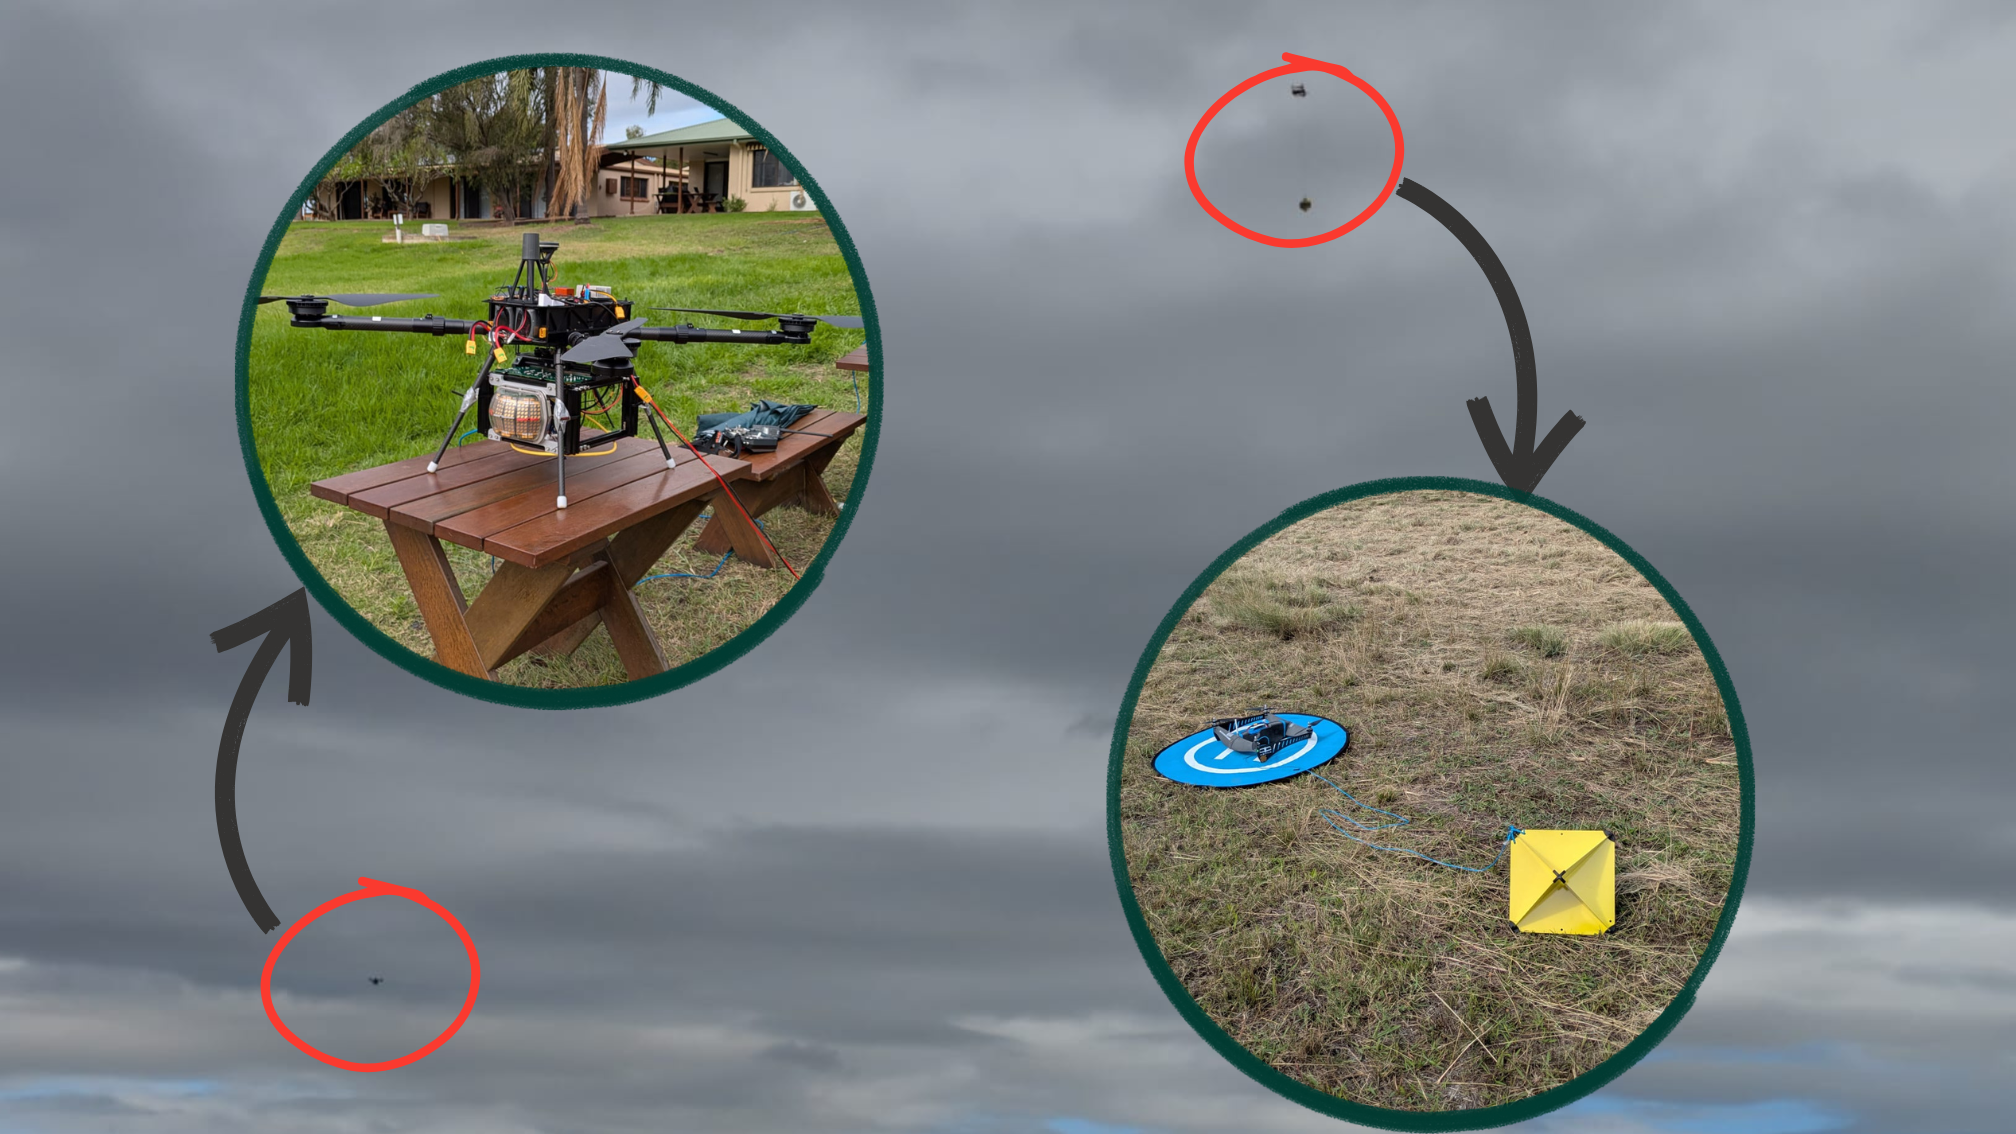
\includegraphics[width=0.6\textwidth]{air-to-air.png}
    \caption{The radar is flown into the air and is pointed at a target drone carrying
    a reflective marker 200m away.}
    \label{fig:real-world-tracking}
\end{figure}

The results of the tracking subsystem failed to produce any tracks of the aerial target, 
due to high coupling between the transmitter and the receiver that saturated the beginning 
of every signal, masking the near-field
where the target was. The radar did detect high cross-section targets 
in the distance (see Figure \ref{fig:field-and-silo}). The detections of these targets are
illustrated in the visualisation of the angle sensing stage
in Figure \ref{fig:points-over-map-singleton}, where detections from the radar line up with
a silo and trees.    

\begin{figure}
    \centering
    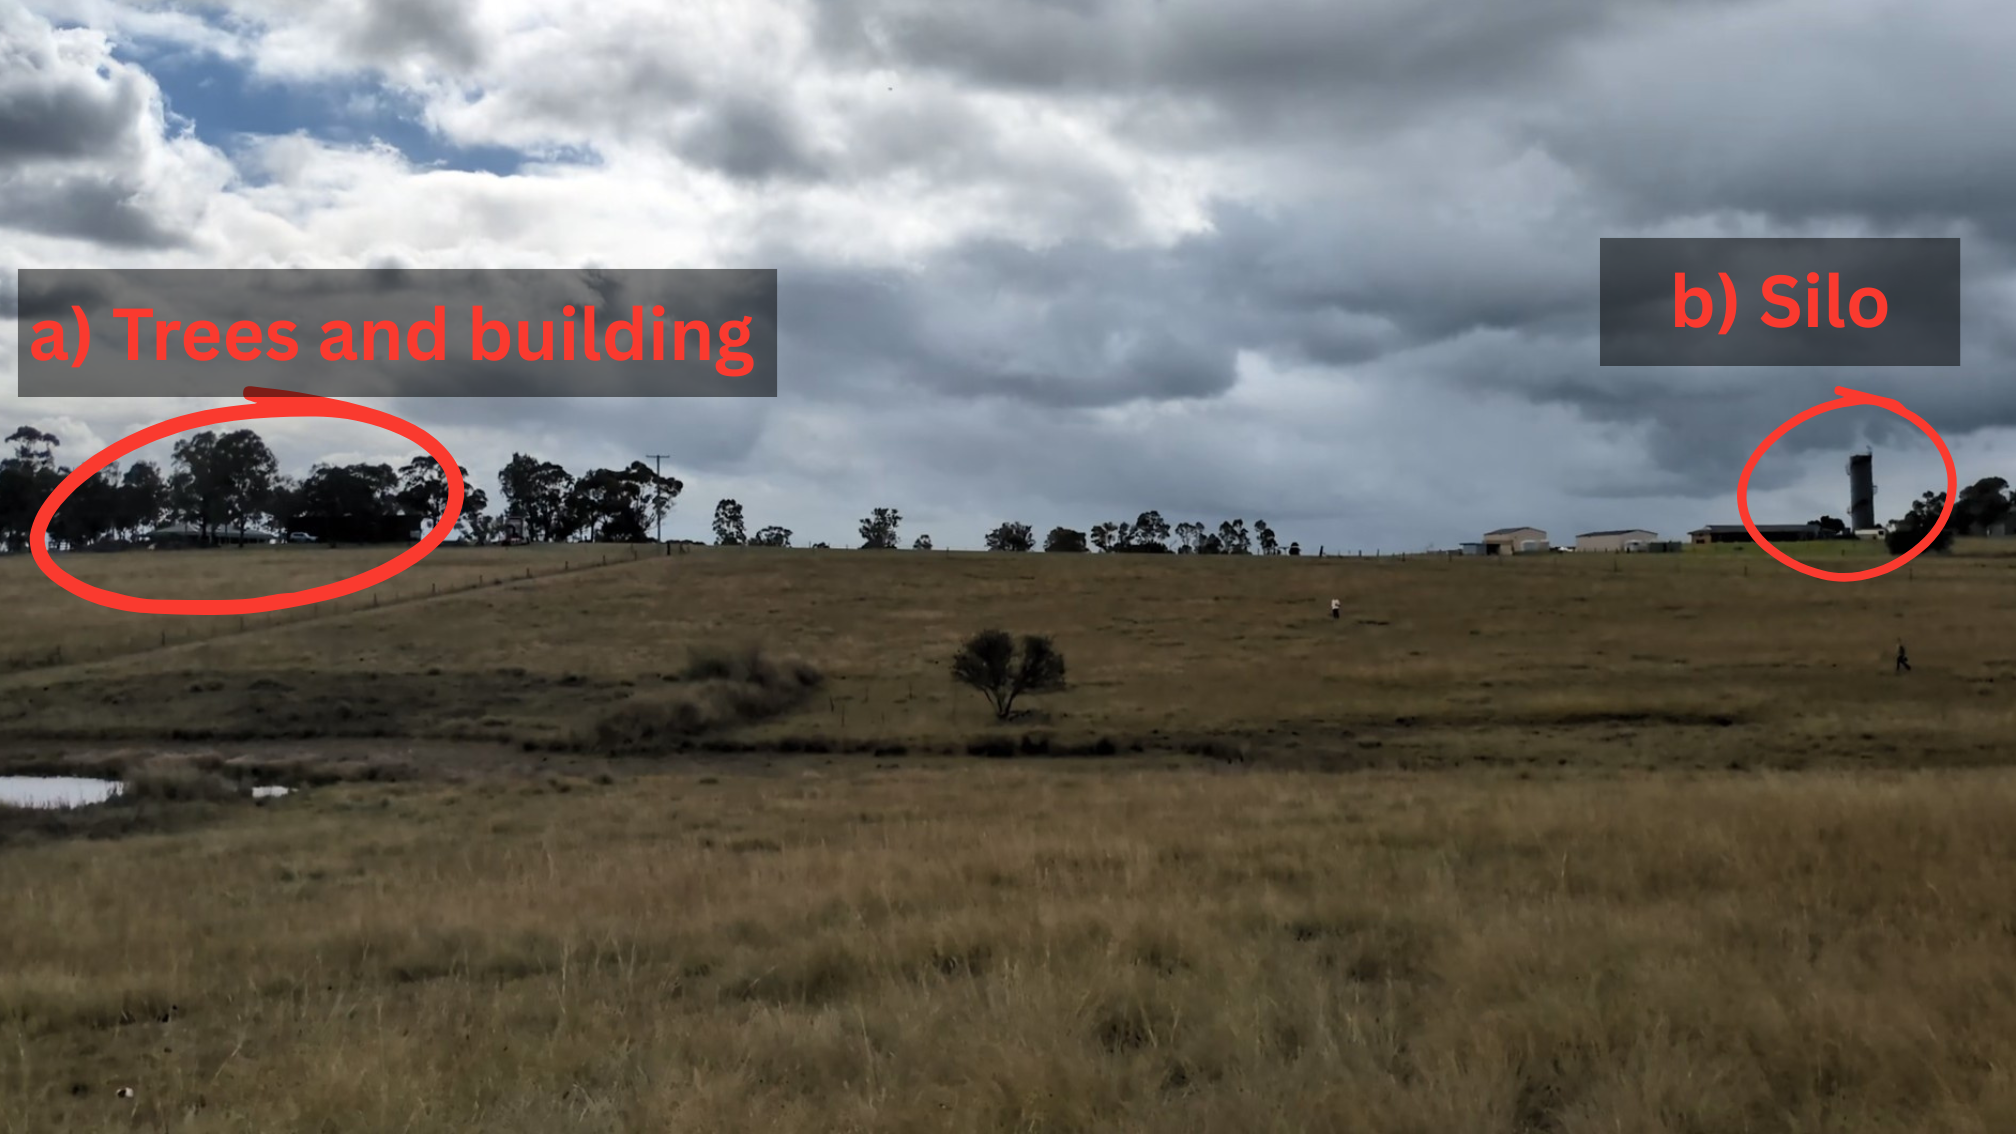
\includegraphics[width=0.6\textwidth]{field-and-silo.png}
    \caption[Radar field of view with silo]{A silo in the distance and a property surrounded by trees are large 
    visible targets for the radar when it is airborne.}
    \label{fig:field-and-silo}
\end{figure}

\begin{figure}
    \centering
    \incfig[0.6]{points-over-map-singleton}
    \caption[Field Trial Silo Detection]{The detected points from the radar are plotted 
    over a map of the area. There is a high correspondence between detected points and
    the three main high cross-section targets in the area: a silo 603 meters away, 
    building 706 m away, and trees surrounding a building 410 meters away. }
    \label{fig:points-over-map-singleton}
\end{figure}

The field trials also provided an opportunity to record realistic noise data, from the open field, and from the radar's own electronics. 
Among the noise was a large DC offset, which produced a peak in the FFT output at 0 Hz, resulting high-power static detections at 
the minimum and maximum range of the radar. This noise was summed with simulated target data to produce D4, one which the whole pipeline was validated 
against in the following section. 

\subsection{Validation in realistic noise}
The pipeline was validated against a dataset D4, which was produced by summing the noise recorded in the field trials with simulated target that
flies in a snaking pattern, sweeping azimuth, elevation and range. Figure \ref{fig:snake} illustrates the ground truth and generated track 
estimations of the snaking target both with and without the realistic noise. Although the signal to noise in both scenarios is held at 0 dB, 
the more irregular noise in the realistic case produces more erratic track estimates, and initiates more false tracks. Despite this,
the tracking subsystem is able to maintain a track of the target.  

\begin{figure}
    \centering
    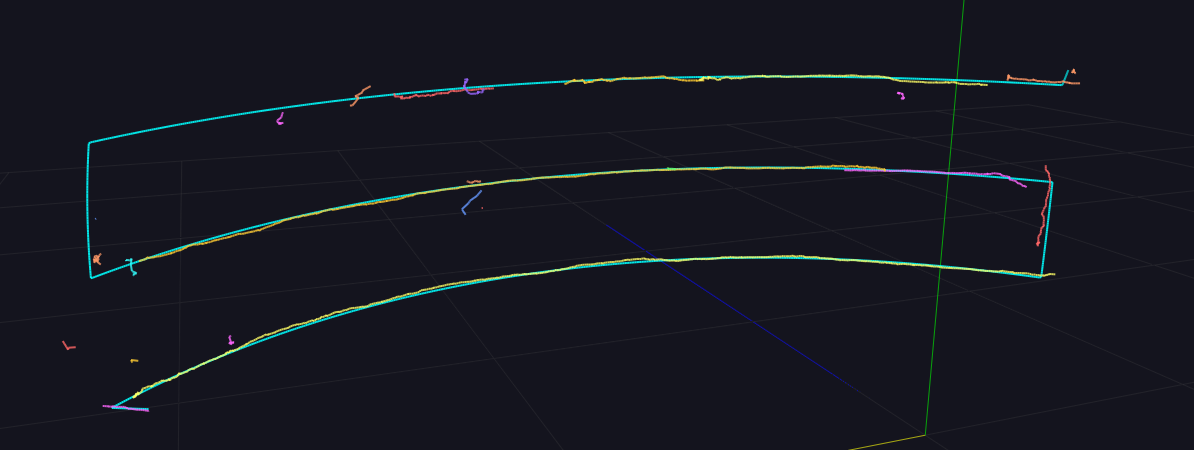
\includegraphics[width=0.7\linewidth]{simulated_snake.png}

    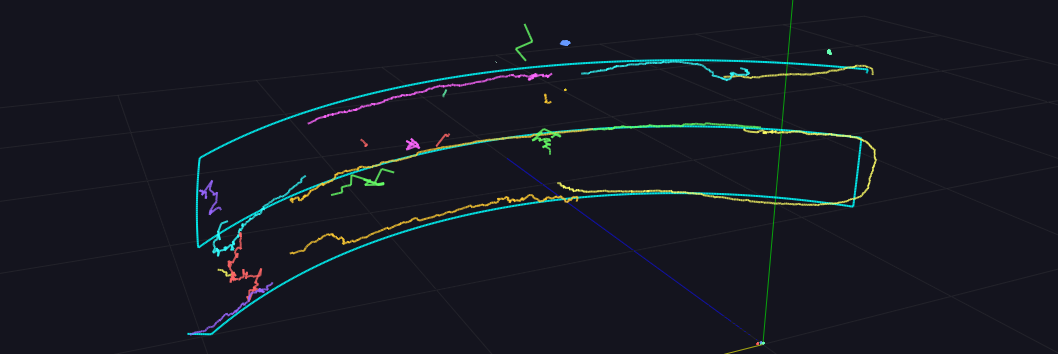
\includegraphics[width=0.8\linewidth]{pseudo_real_snake.png}
    \caption[Tracking a snaking target with and without realistic noise.]{Ground truth
    and track estimates for a target flying a snaking pattern at 0\,dB SNR. The images
    depict just a single range for clarity. The ground truth is depicted in blue while
    a line of a given colour represents an unbroken track. Top: with
    purely simulated noise. Bottom: with realistic noise recorded during field trials
    summed with the simulated target. The realistic noise produces more erratic track
    estimates and initiates more false tracks, though the tracker maintains a track of
    the target throughout.}
    \label{fig:snake}
\end{figure}


\FloatBarrier
\section{Windowing}
The Hann (with $\alpha = 0.5$) and Hamming windows are first evaluated for the prominence of their main lobe and sidelobes
in the frequency domain on the synthetic datasets. Figure \ref{fig:clean filters} illustrates the 
performance of each of the filters on a clear sine wave with no noise. Figure \ref{fig:noisy filters}
illustrates the performance of each of the filters on the noisy simulated data with an SNR of 1.  

\begin{figure}
    \incfig[0.7]{filter_clear_comparison}
    \caption[Window filter comparison on a noise-free signal.]{Results of an \gls{fft} performed on a single frequency signal without noise without a filter,
    with a Hann window, and a Hamming window. Each of the tests correctly produces a peak near
    bin 334, the target range. The no filter option's peak is wider than the filtered options.
    The Hann window performs the best globally, with a 100 dB reduction in power when more than 40
    bin away from the target bin. The Hamming window performs significantly worse globally, with
    only a 70 dB reduction when more than 40 bins away, but has a steeper drop-off near the
    target bin, which may result in better resolution of closely spaced targets.}
    \label{fig:clean filters}
\end{figure}

\begin{figure}
    \incfig[0.7]{filter_noisy_comparison}
    \caption[Window filter comparison at SNR of 1.]{Results of an \gls{fft} performed on a single frequency signal with an SNR of 1 with no
    window filter, with a Hann window filter, and a Hamming window filter. The no filter option's
    spectral leakage acts to deform the peak at bin 334. The Hann and Hamming windows perform similarly
    globally but the Hamming window features a slightly higher peak, and less spectral leakage into
    the adjacent bins.}
    \label{fig:noisy filters}
\end{figure}

In terms of computational performance, the latency contribution of the filters does not significantly 
differ across implementations. Figure \ref{fig:latency} shows the time taken to process
a single frame of 10 000 chirps each with 767 samples, averaged over 50 runs. 

\begin{figure}
    \incfig[0.7]{filter_latency_comparison}
    \caption[Windowing stage latency across implementations.]{Latency contribution of the windowing stage to the overall pipeline. The latency does not
    significantly differ across implementations, with all implementations taking around 9-12 ms to
    process 7 670 000 samples. The insignificant difference in latency between no filter
    and filters suggests that the delay is primarily due to the overhead of handling the data.}
    \label{fig:latency}
\end{figure}

The experiments were then extended to the Blackman, Kaiser, and Taylor windows. Using dataset DS2,
the multi-receiver signal of a target sweep azimuth, elevation and range, fifteen filter 
configurations were applied to the data: \verb|Hann|, \verb|Hamming|, \verb|Blackman|, 
\verb|Kaiser6|, \verb|Kaiser8|, \verb|Kaiser10|, \verb|Kaiser12|, \verb|Taylor1_30|, 
\verb|Taylor2_30|, \verb|Taylor_3_30|, \verb|Taylor_4_30|, \verb|Taylor1_50|, \verb|Taylor2_50|
\verb|Taylor_3_50|, \verb|Taylor_4_50|. The parameter suffix of the Kaiser windows indicate the 
\(\beta\) parameter and the two suffixes of the Taylor windows indicate \(\bar{n}\) and the 
sidelobe level in -dB respectively.  

Six noise intensities were applied to the data: no noise, and SNRs of -20, -10, 
0, 10 and 20 dB. Detections at ranges where the target is not were labelled as clutter, they 
were tallied and their total power was recorded. Figures \ref{fig:recall_vs_clutter} and 
\ref{fig:recall_vs_clutter_power} illustrate the relationship between noise, windows, and their
effect on recall and clutter.  

\begin{figure}
    \incfig[0.8]{windowing_recall_vs_clutter}
    \caption[Recall vs clutter for different window functions.]{Recall vs clutter for different 
    window functions. The recall of the target detections decreases from 1 to 0.45 with increasing 
    noise, and the number of clutter detections increases with increasing noise from 3 to 12 per 
    actual truth. Window choice trades less clutter for sensitivity. The Taylor windows calibrated
    to -50dB noise achieve high recall without introducing more clutter than the other windows. The choice of window does 
    not significantly affect recall or clutter, though the Hamming window performs slightly 
    better at high SNRs.}
    \label{fig:recall_vs_clutter}
\end{figure}

\begin{figure}
    \incfig[0.8]{windowing_recall_vs_clutter_power}
    \caption[Recall vs clutter power for different window functions.]{Recall vs clutter power 
    for different window functions. While producing slightly higher clutter power, the four 
    -50 dB Taylor windows achieve higher recall than the other windows in the three noisiest 
    conditions.}
    \label{fig:recall_vs_clutter_power}
\end{figure}

\FloatBarrier
\section{Integration}
The integration stage is validated on synthetic test data from software scripts and the 
test-source mode of the AWR2243 radar chips. The results from the former illustrate the expected increase
in SNR with increasing integration window size as demonstrated in Figure \ref{fig:integration-waterfall}. 
The results from the latter illustrate no increase in SNR because the test-source mode does not generate 
any noise. Meaningfully, the results from the AWR test-source mode indicate that the integration stage 
behaves correctly on data from the radar chips, (see Figure \ref{fig:integration-waterfall-orac}). The 
subsystem can process the data at a rate of 9.8 times the incoming data rate on the desktop setup, and 
3.8 times the incoming data rate on the Xavier setup. We also find that the latency of the integration 
stage increases with the integration's factor of reduction, since in our implementation,
each thread performs all the sum operations for its corresponding range bin
(which increases with the reduction factor of the integration stage). 


\begin{figure}
    \incfig[0.57]{integration_waterfall}
    \caption[Integration on synthetic data showing SNR improvement.]{Results of the integration stage on synthetic data.
    The top window shows a low SNR waterfall plot of data, with the y-axis
    representing range samples and
    the x-axis representing chirps that are streaming into the integration stage. The
    colour indicates the power of the range bin, with yellow being the most intense.
    The output of the integration stage below has less noise, and the target
    signal is more prominent.} 
    \label{fig:integration-waterfall}
\end{figure}

\begin{figure}
    \incfig[0.57]{integration_waterfall_orac}
    \caption[Integration on AWR2243 test-source data.]{Results of the integration stage on AWR2243 test-source data.
    The 8 windows correspond to 8 channels. 128 chirps are being compressed into a single
    chirp with no noise. There is
    no change in amplitude, validating that the integration stage behaves
    correctly on radar chip data.}
    \label{fig:integration-waterfall-orac}
\end{figure}

The latency of the integration stage increases with the reduction factor of the integration stage,
as demonstrated in Figure \ref{fig:ablation-cumulative-latency}. Many of this latency is due to 
the overhead associated with handling the data and the launching the application. By finding the 
time taken
to process as a function of the number of input frames we can approximate the startup time of the 
pipeline and subtract it from the total time to find the time taken to process each frame. 
This is done with coherent integration, non-coherent integration, and no integration as a 
baseline. 
Additionally, for this trial, the pipeline has been patched to not input or output any data, just processing
empty buffers, which allows us to avoid measuring the overhead of handling the data.  

\begin{figure}
    \incfig[0.7]{integration_throughput}
    \caption[Integration stage latency per frame.]{Processing time as a function of the number 
    of input frames. The startup time of the pipeline is approximated 
    by finding the y-intercept of the line of best fit, which is 195 ms for all three scenarios. 
    The figure also illustrates that there is only a small difference between the processing time
    of either integration strategy and no integration at all, with the non-coherent integration
    taking 0.02 milliseconds more per frame than no integration, and the coherent integration. 
    }
    \label{fig:integration-latency-per-frame}
\end{figure}

Dataset DS2 sweeps az el and range in the six noise regimes, -20, -10, 0, 10 and 20dB SNR and no noise. 
SNRs were tuned to detections at the further ranges. Closer detections have higher SNRs than 
what is listed. 
Figure \ref{fig:integration-setup} illustrates the ground truths and 64 detections per ground truth
for one of the noisy scenarios. 

\begin{figure}
    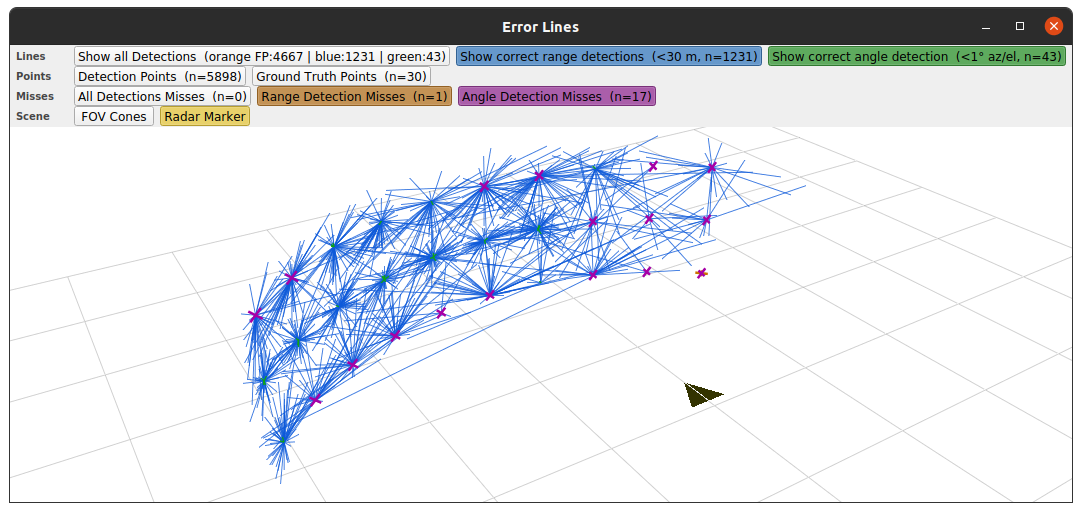
\includegraphics[width=0.9\textwidth]{integration_setup.png}
    \caption[Integration experiment ground truths and detections.]{The setup of the integration 
    stage experiment for accuracy evaluation. The figure shows the detections of a target 
    sweeping azimuth, elevation and range in a noisy scenario. Each line segment indicates the 
    ground truth on one end and the detection on the other. Purple crosses indicate ground 
    truths with no detections within 1 degree in azimuth and elevation of them. The triangle 
    marks the radar position and heading.}
    \label{fig:integration-setup}
\end{figure}

The results of the experiment are illustrated in Figures 
\ref{fig:integration-angle-recall-per-segment} and
\ref{fig:integration-RMS-position-error}.

\begin{figure}
    \incfig[0.9]{integration_angle_recall_per_segment}
    \caption[Recall Integration Experiment.]{Recall, the proportion of ground truths 
    with at least one detection within 1 degree in azimuth and elevation of them, of 
    the integration stage experiment as the integration length (number of chirps integrated
    together) increases, for both coherent and non-coherent integration in the six noise 
    intensities. As the integration length increases, the recall of the detections increases,
    with the coherent integration performing consistently better than the non-coherent integration
    across all noise intensities. Through coherent integration of 64 chirps, the recall in the 
    worst noise regime increased from near 0 to 0.9.}
    \label{fig:integration-angle-recall-per-segment}
\end{figure}

\begin{figure}
    \incfig[0.9]{integration_RMS_position_error}
    \caption[Position Error Integration Experiment.]{RMS position error of the integration 
    stage experiment as the integration length (number of chirps integrated together) increases, 
    for both coherent and non-coherent integration in the six noise intensities. The figure 
    shows that integration directly improves position accuracy, with coherent integration 
    performing slightly better than non-coherent integration when the 
    integration length is larger than 4. }
    \label{fig:integration-RMS-position-error}
\end{figure}


\FloatBarrier
\section{Constant False Alarm Rate}
\subsection{Correctness}
Under the assumption of an 8-degrees of freedom chi-squared distribution of sample noise 
power for a given quadruplet of receivers, the CFAR threshold coefficient $\alpha$ is 
calculated numerically for a range of false alarm 
rates. The actual false alarm rate is then measured by running the CFAR algorithm on a noise-only
synthetic dataset. Figure \ref{fig:alpha-cfar-results} illustrates the results.

\begin{figure}[htbp]
    \centering
    \incfig[0.4]{pfa_comparison} 
    \caption[Actual vs desired false alarm rate validating the numerical CFAR threshold.]{The actual 
    false alarm rate closely matches the desired false alarm rate across a range
    of false alarm rates. The numerical solution for $\alpha$ is therefore accurate under the assumption
    of an 8-degrees of freedom chi-squared distribution of sample noise power across a quadruplet of 
    receivers.}
    \label{fig:alpha-cfar-results}
\end{figure}

The results indicate that the numerical solution for $\alpha$ is accurate, with the actual false alarm 
rate closely matching the desired. The successful performance of CFAR with a false alarm rate of 
\(0.001\) is illustrated in Figure \ref{fig:cfar-0.001-waterfall}.

\begin{figure}[htbp]
    \centering
    \incfig[0.8]{cfar-0.001-waterfall}
    \label{fig:cfar-0.001-waterfall}
    \caption[CFAR waterfall at false alarm rate of 0.001.]{CFAR with a desired false alarm rate of \(0.001\) infrequently detects peaks in what is
    predominantly noise, as expected. The figure is a waterfall plot, with chirp on the y-axis and range
    on the x-axis. The brightness of the cell reflects the power of the corresponding chirp's range bin.
    The black space indicates that most cells are masked by CFAR.} 
\end{figure}

\subsection{Computational Performance}
The speed of each of the three CFAR implementations is measured across a range of buffer sizes, from 
one frame of 767 samples, to 4042 frames of 767 samples. This sweep is performed on both the desktop 
and the Xavier. The results are illustrated in Figures \ref{fig:cfar-implementation-performance-Xavier} 
and \ref{fig:cfar-implementation-performance-desktop}.

\begin{figure}[htbp]
    \centering
    \includesvg[width=0.75\linewidth]{CFAR implementation speed on desktop.svg} 
    \caption[CFAR implementation speed vs buffer size on the desktop.]{Computational Performance of three CFAR implementations as a function of buffer size on the
    desktop setup. The CPU implementation with a prefix sum tables is the fastest for small buffer sizes,
    but the GPU implementation is slightly faster for larger buffer sizes. The naive CPU implementation
    is the slowest across all buffer sizes.}
    \label{fig:cfar-implementation-performance-desktop}
\end{figure}

\begin{figure}[htbp]
    \centering
    \includesvg[width=0.75\linewidth]{CFAR implementation speed on Xavier.svg} 
    \caption[CFAR implementation speed vs buffer size on the Xavier.]{Computational Performance of three CFAR implementations as a function of buffer size on the
    Xavier NX setup. The CPU implementation with a prefix sum tables is the fastest for small buffer sizes,
    but the GPU implementation is slightly faster for larger buffer sizes. The naive CPU implementation
    is the slowest across all buffer sizes.}
    \label{fig:cfar-implementation-performance-Xavier}
\end{figure}

The speed is also plotted as a function of the number of CFAR training cells. The results are illustrated 
in Figures \ref{fig:cfar-implementation-performance-Xavier-training-cells} and 
\ref{fig:cfar-implementation-performance-desktop-training-cells}. The desktop results illustrate that both
the GPU and the prefix sum table implementations are not significantly affected by the number of training
cells, while the naive CPU implementation's speed increases linearly with the number of training cells. 
The Xavier results illustrate that while the prefix sum table implementation remains invariant to the 
number of training cells (as we expect), the GPU implementation's speed does increase with the number 
of training cells, due to the fact that each thread has more work to do to calculate the noise statistic. 
Results on the Xavier show that the GPU implementation is faster than either CPU implementation 
for window sizes within the practical range of 10 - 100 training cells.  

\begin{figure}
    \centering
    \includesvg[width=0.8\linewidth]{CFAR implementation speed over window size 10.svg} 
    \caption[CFAR implementation speed vs training cells on the desktop.]{Computational Performance of three CFAR implementations as a function of the number of
    training cells on the Desktop Setup. Buffer size is fixed at 10 quadruplet chirps per frame.}
    \label{fig:cfar-implementation-performance-desktop-training-cells}
\end{figure}

\begin{figure}
    \centering
    \includesvg[width=0.8\linewidth]{CFAR implementation speed over window size 10 Xavier.svg} 
    \caption[CFAR implementation speed vs training cells on the Xavier.]{Computational Performance of three CFAR implementations as a function of the number of
    training cells on the Xavier Setup. Buffer size is fixed at 10 quadruplet chirps per frame.}
    \label{fig:cfar-implementation-performance-Xavier-training-cells}
\end{figure}

Three implementations of CFAR, CA-CFAR, GO-CFAR, and SO-CFAR, were tested on the DS2 dataset with
six different noise intensities: no noise, -20, -10, 0, 10 and 20dB SNR. Figure 
\ref{fig:cfar-recall} illustrates the recall, the number of 
ground truth range bins with a detection within them, and clutter to signal
ratio as a function of noise and CFAR algorithm. Figure \ref{fig:cfar-clutter-to-signal} 
illustrates the clutter to signal ratio of each of the CFAR algorithms as noise increases, 
and Figure \ref{fig:cfar-position-error} illustrates the RMS position error of the true 
positives of each of the CFAR algorithms as noise increases.  

\begin{figure}
    \centering
    \incfig[0.8]{cfar_recall} 
    \caption[CFAR recall vs noise and algorithm.]{Recall of three CFAR algorithms as a 
    function of noise. The figure shows that the recall decreases with increasing noise, 
    and that CA-CFAR features the lowest clutter power for the noisiest regimes.}
    \label{fig:cfar-recall}
\end{figure}

\begin{figure}
    \centering
    \incfig[0.8]{cfar_clutter_to_signal} 
    \caption[CFAR clutter to signal ratio vs noise and algorithm.]{Clutter to signal 
    ratio of three CFAR algorithms as a function of noise. The figure shows that the 
    clutter to signal ratio increases with increasing noise, and that CA-CFAR 
    features the lowest clutter power for the noisiest regimes, while GO-CFAR 
    performs well in the low noise intensities.}
    \label{fig:cfar-clutter-to-signal}
\end{figure}

\begin{figure}
    \centering
    \incfig[0.8]{cfar_position_error} 
    \caption[CFAR position error vs noise and algorithm.]{RMS position error of the 
    true positives of three CFAR algorithms as a function of noise. The figure shows 
    that the position error increases with increasing noise, and that all CFAR 
    algorithms perform with similar accuracy. CA-CFAR features slightly better 
    accuracy in the noisiest regimes }
    \label{fig:cfar-position-error}
\end{figure}

\subsection{Clustering}
The clustering stage is validated on the DS2 dataset with no noise. The ground truths are 
depicted in Figure \ref{fig:angle-3d-plot}. The results are illustrated
in Figure \ref{fig:clustering-results}. The figure shows that the clustering stage successfully
maps contiguous blocks of detected range bins into single detections with continuous
range. 

\begin{figure}
    \centering
    \incfig[0.9]{cluster-experiment}
    \caption[Clustering results on the DS2 dataset with no noise.]{Clustering results on the 
    DS2 dataset with no noise. The figure shows that the clustering stage successfully
maps contiguous blocks of detected range bins into single detections with continuous
range. The y-axis is time and the x-axis is range. The colour is amplitude. The bright 
pink line in the first two subplots corresponds to the green and yellow line in the cluster 
output.}
    \label{fig:clustering-results}
\end{figure}


\subsection{Monopulse Angle Sensing}
\subsection{Correctness}
With the same DS2 dataset from the CFAR evaluation with 0 noise, the monopulse angle sensing 
algorithm is validated by comparing it's azimuth and elevation estimates to the ground truth. 
The results are illustrated in Figures \ref{fig:angle-polar-error} and 
\ref{fig:angle-3d-plot}. Seeing low error suggests that the monopulse angle sensing is 
correctly applying the reverse transformation that the radio wave simulation piece utilised
to convert position to multi-change signal data. 

\begin{figure}
    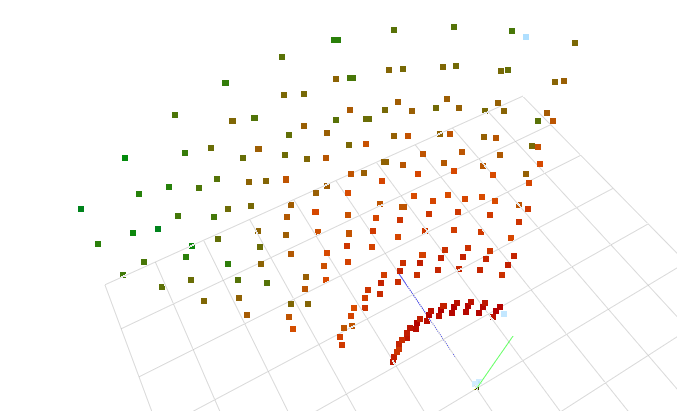
\includegraphics[width=0.8\textwidth]{angle-ground-truth-3d.png}
    \centering
    \caption[Angle experiment Ground Truth 3D plot]{The ground truth measurements of the angle sensing DS2
    dataset plotted in 3D. Points are coloured by signal strength and points are arranged in a 
    polar array.}
    \label{fig:angle-3d-plot}
\end{figure}

\begin{figure}
    \incfig[0.8]{angle_polar_error_scatter_plot}
    \centering
    \caption[Monopulse angle sensing polar error scatter plot.]{Polar error scatter plot
    of the monopulse angle sensing algorithm on the DS2 dataset with 0 noise. The figure 
    shows that the polar error of the angle estimates is generally below 0.3 degrees in 
    az el and rng and the range error is less than 1.5 meters over the tested range. } 
    \label{fig:angle-polar-error}
\end{figure}

Under -10dB SNR, the 3D plot view fills up with clutter and angle sensing accuracy 
quickly degrades. But plotting the amplitude of the detections and accumulating 
detections over 64 chirps per grid position in the dataset, clusters around the 
true target positions can be visually identified, validating the effectiveness of 
monopulse angle sensing in high noise conditions (calculated azimuth and elevation
seem to be unbiased estimators of the true azimuth and elevation). The phenomenon 
is illustrated in Figure \ref{fig:angle-3d-plot-noise}.

\begin{figure}
    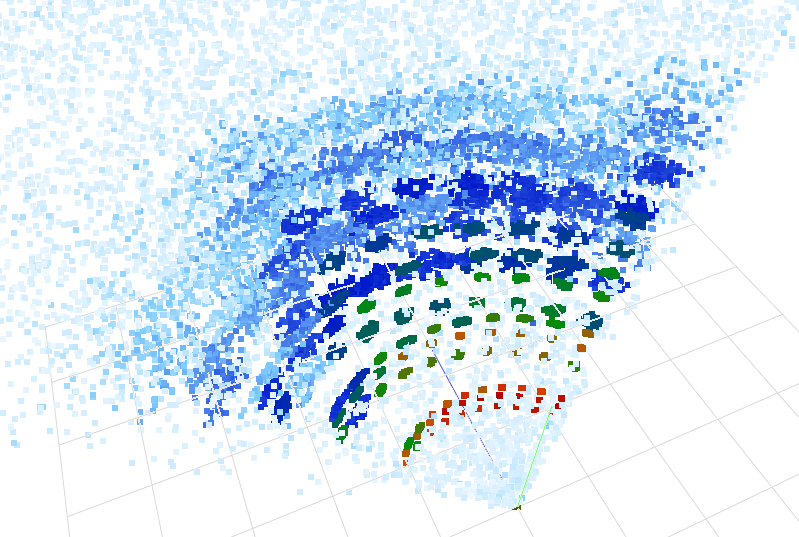
\includegraphics[width=0.7\linewidth]{angle squares light mode noisy.png}
    \caption[Monopulse angle sensing 3D plot with noise.]{3D plot of the monopulse 
    angle sensing algorithm on the DS2 dataset with -10dB SNR at max range. The 
    figure shows the 
    degradation in angle sensing accuracy under high noise conditions as range increases}
    \label{fig:angle-3d-plot-noise}
\end{figure}

To understand the failure modes of monopulse angle sensing for multiple targets, 
a simulation tool was built to validate the monopulse angle sensing algorithm on 
synthetic data. The tool allows the 
user to create multiple targets, and specify the bearing/elevation ratios of each 
target. The simulated data is then 
processed by the preprocessing subsystem, the aggregator, CFAR, and the monopulse 
angle sensing algorithm. The 
resulting angle estimates are visualised live in a 3D plot. A frame of this view is 
illustrated in Figure 
\ref{fig:monopulse-angle-sensing-results}.

\begin{figure}
    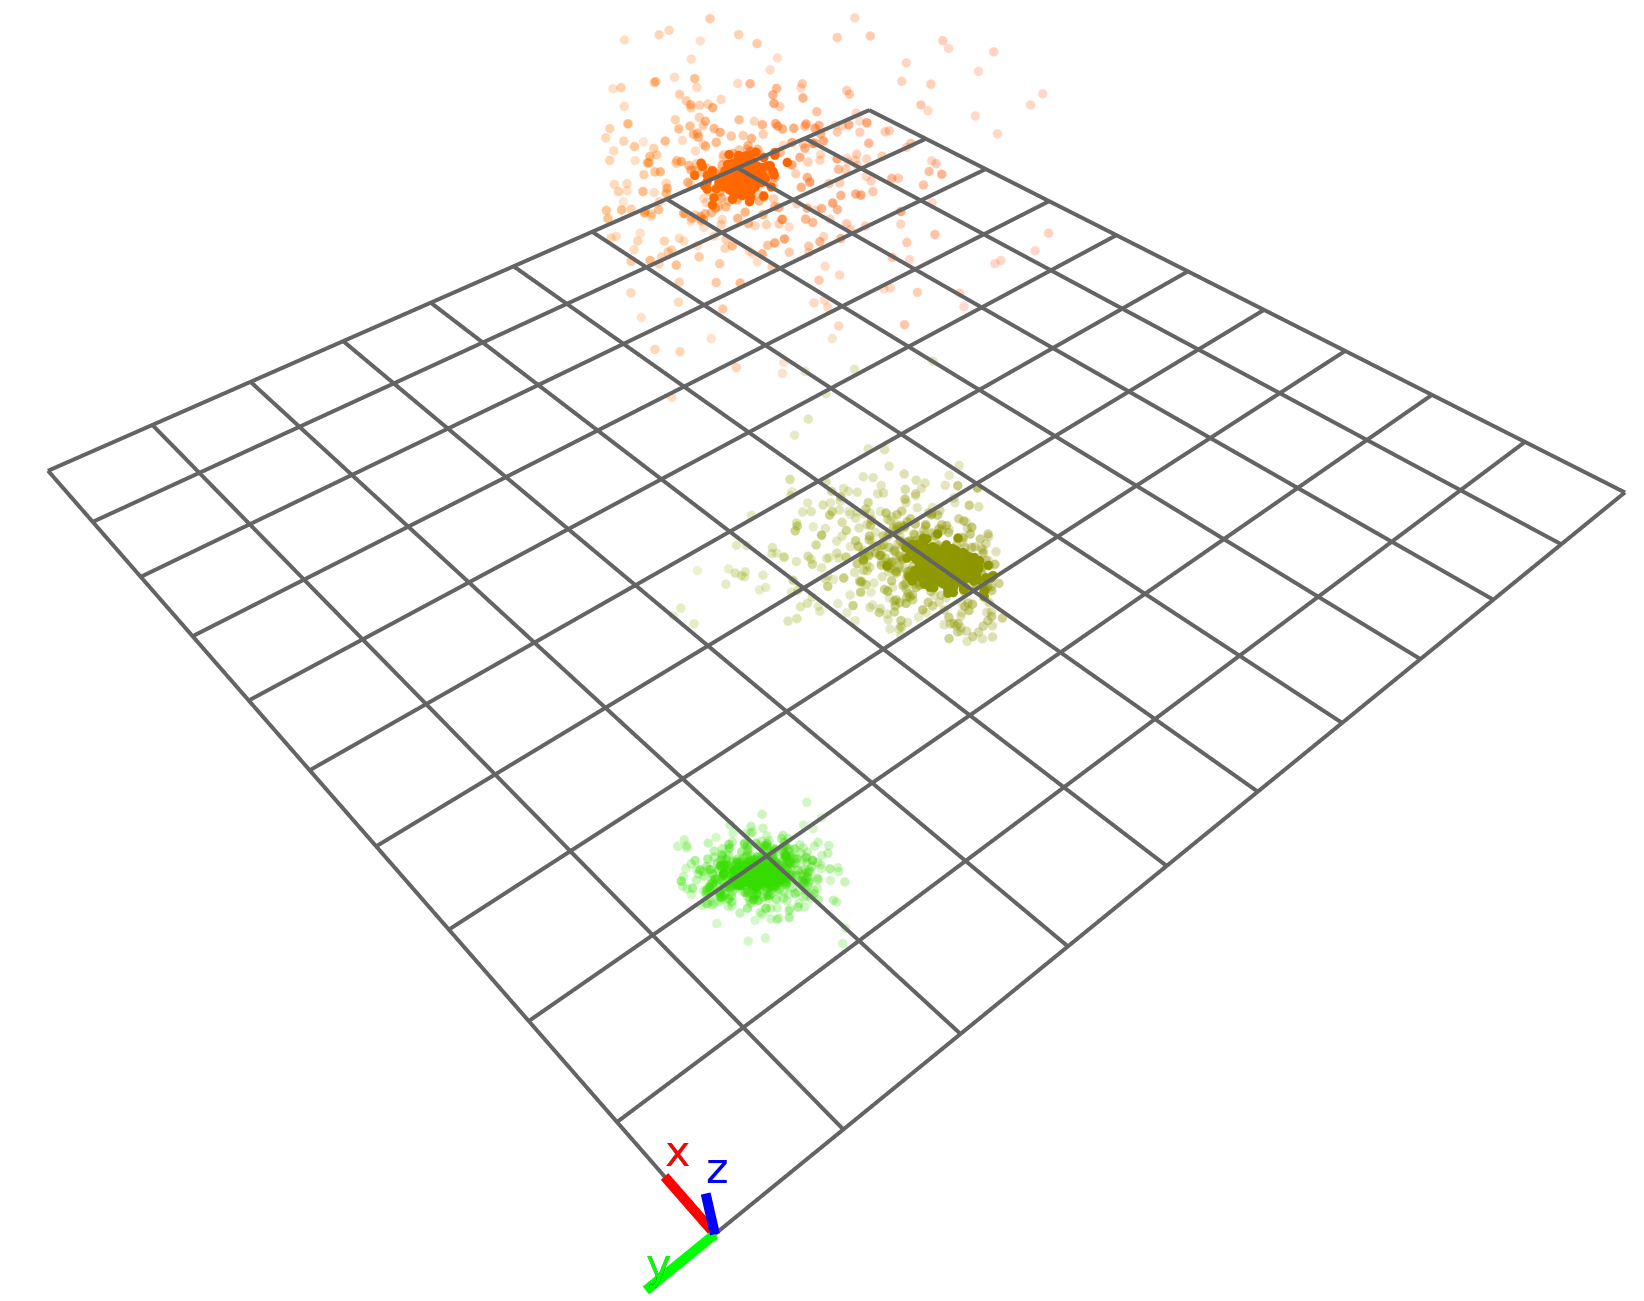
\includegraphics[width=0.8\linewidth]{monopulse_angle_sensing_results.png}
    \caption[Monopulse angle sensing results on synthetic data.]{Results of the monopulse angle sensing algorithm on synthetic data. The colour of the dots indicate
    the range of the detections, with green being close and orange being far away. The opacity of the dots indicate
    the strength of the detections, with more opaque dots being stronger. The plot features the most recently 1000
    detections. The spread of the dots increases with range as expected, and the
    upper and lower bounds of elevation and bearing match the field of view
    defined by the calibration polynomial.}
    \label{fig:monopulse-angle-sensing-results}
\end{figure}

The relative latency cost of the angle and CFAR operations were measured through an ablation study on the detection 
subsystem. The results are illustrated in Figure \ref{fig:tracking-latency-trials} which shows the latency 
of just CFAR, just angle sensing, and both, and Figure \ref{fig:tracking-latency-breakdown}. 

\begin{figure}
    \includesvg[width=0.8\linewidth]{tracking_latency_trials.svg}
    \caption[Detection subsystem latency for CFAR, angle sensing, and both.]{Latency of the subsystem running CFAR, angle sensing, and both on a log scale.
    The latency of the subsystem
    running CFAR is similar to the latency of the subsystem running both, while angle sensing
    is 1.5-5 times faster than either,
    suggesting that CFAR dominates the latency of the subsystem.}
    \label{fig:tracking-latency-trials}
\end{figure}

\begin{figure}
    \includesvg[width=0.8\linewidth]{tracking_latency_breakdown.svg}
    \caption[Detection subsystem latency breakdown from ablation study.]{A breakdown of the latency of the subsystem estimated from the ablation study.
    Most of the latency is split
    between CFAR and the overhead of handling the data, which involves synchronising threads
    and migrating data between the CPU and GPU.}
    \label{fig:tracking-latency-breakdown}
\end{figure}

The angle stage has no parameters to tune other than the coefficients of the calibration
polynomial, which are determined by the beam shape of the receivers. Therefore, the latency 
and correctness analysis is all that can be done. 

\subsection{Tracking}
To validate the tracking stage, 12 scenarios were selected from the DS2 dataset. 
These scenarios involve 1, 2 and 3 targets at no noise, -20, -10, and 0 SNR. Figures 
\ref{fig:tracking-initiation-accuracy} and \ref{fig:tracking-position-accuracy} 
demonstrate the effect of noise and target count on track initiation accuracy, 
position accuracy, and track health.  

%include 4 figures
% track_basic_stats
% track_MOTA_stats
% track_RMS Angle Error
% track_RMS Distance

\begin{figure}
    \incfig[1]{track_basic_stats}
    \caption[Tracking initiation accuracy and track health.]{Tracking accuracy and 
    track health across 12 scenarios with different noise and target count. The figure shows 
    that track-level accuracy, precision, recall, are highest when there is some noise, and 
    only one target. Point level accuracy, precision and recall are also highest in that 
    scenario.}
    \label{fig:tracking-initiation-accuracy}
\end{figure}

\begin{figure}
    \incfig[1]{track_MOTA_stats}
    \caption[Tracking MOTA (Multi-Object Tracking Accuracy) statistics.]{MOTA is highest in the presence of some 
    noise and one target. MOTP (Multi-Object Tracking Precision) strictly increases with noise for all target 
    counts. Mean completeness, mean delay until initiation, fragmentation, and survival 
    ratio are also depicted. }
    \label{fig:tracking-position-accuracy}
\end{figure}

\begin{figure}
    \incfig[0.8]{track_RMS_Angle_Error}
    \caption[Tracking RMS angle error.]{Tracking RMS angle error across 12 scenarios 
    with different noise and target count. The figure shows that RMS angle error 
    degrades with increasing noise and target count.}
    \label{fig:tracking-angle-error}
\end{figure}

\begin{figure}
    \incfig[0.8]{track_RMS_Distance}
    \caption[Tracking RMS distance error.]{Tracking RMS distance error across 12 scenarios 
    with different noise and target count. The figure shows that RMS distance error 
    degrades with increasing noise and target count.}
    \label{fig:tracking-distance-error}
\end{figure}

% Here include basic stats and fancy stats. 
% Talk more about random targets instead of sweep
% Show the ground truth for three targets and some view-tracks.py images. 
% Get everyone to understand how much the tracking stage is doing.


 
\chapter{Discussion}
In this chapter, we discuss the key findings within the results of the 
experiments. Then we discuss shortcomings of the research so far. Lastly,
recommendations are given. 

\section{Findings}
The results of the testing on the windowing function confirm the 
consensus in the literature, that the Hann and Hamming windows 
are both
effective in reducing spectral leakage when compared to no window. 
Through comparing the two windows, we find that the Hamming 
window is more appropriate 
for radar purposes with its sharper drop-off that allows detection to 
be more precise, at the cost of more global spectral leakage. 
Additionally, the insignificant
time difference between either window or no window is expected given
the simplicity of the function, with each kernel performing just one
multiplication. The negligible latency difference across the desktop and Xavier
platforms further indicates that window selection can be made independently of
hardware configuration. The differing spectral leakage patterns motivate a more
comprehensive search for window functions that are most appropriate for
miniature radar applications. 

The results from the coherent integration experiment find that the signal 
to noise ratio improves by the square root of the number of chirps summed 
together under Gaussian noise, creating a positive downstream effect on the 
ability of CFAR to detect weak 
targets. The difference in throughput of the processing subsystem on 
the desktop versus the Xavier is likely due to the overhead of handling data,  
such as reading and writing. The large amount of work that each thread has to 
do, summing over many chirps, motivates the exploration of more parallelised 
implementations that distribute the sums between threads. 

The CFAR results outline a method for determining a threshold from a 
desired false alarm rate. The experiments demonstrate the GPU implementation
is most appropriate for the Xavier embedded platform, regardless of the size 
of the buffer for all practical window sizes. The difference between hardware
platforms highlights the importance of hardware-aware algorithm selection. The 
results of the angle sensing stage demonstrate the capability of the algorithm 
to detect multiple targets with different bearing/elevation ratios. The ablation 
study illustrates that CFAR dominates the latency 
of the tracking subsystem. The relatively high cost of CFAR motivates the exploration
of more efficient CFAR implementations. Potential approaches include implementing 
the prefix sum table approach on the GPU, using a reduction approach to calculate the 
noise floor, and more consciously minimising cache misses within warps. 

The completed results begin to address two of the three research gaps identified in the
literature review. The GPU pipeline benchmarking across desktop and Xavier platforms, covering CFAR, angle
sensing, windowing, and coherent integration, directly addresses
gap 2, providing the hardware-validated latency, throughput, and architectural profiling
that prior UAV DAA radar work lacked. The hardware-aware implementation comparisons
partially address gap 3, establishing a baseline for angle sensing performance, though
evaluation under realistic multi-target and non-Gaussian noise conditions remains to be
completed. Gap 1, concerning detection sensitivity against small moving airborne targets,
and the remaining scope of gap 3, require the tracking stage and real flight data, which
are the subject of the remaining work.

\section{Shortcomings}
The project has progressed broadly in line with the initial proposal, with the 
preprocessing subsystem, CFAR detection, monopulse angle sensing, and the supporting 
simulation and profiling infrastructure all implemented and evaluated. The pipeline 
architecture has been validated on both synthetic data and real AWR2243 hardware data, 
and hardware-aware implementation comparisons have been completed for the CFAR stage 
across the desktop and Xavier platforms.

Several goals from the initial proposal were not completed within this reporting period.
The multi-target tracking stage, comprising clustering and the tracking filter, was not
implemented or evaluated. This represents the most significant deviation from the
proposed plan, and means that the end-to-end pipeline remains incomplete and that track
quality cannot yet be used as an evaluation metric. The primary cause of this delay was
the time required to bring up the hardware pipeline and validate each stage on real radar
data. The remaining work in the project plan is structured to address this directly.
Until the tracking stage is complete, gap 1 (detection sensitivity against small moving
airborne targets) cannot be addressed, as it requires track-level performance metrics
from real encounter scenarios.

% Incorrect below
The window function evaluation was narrowed to Hann and Hamming windows, deferring the
evaluation of Blackman, Kaiser, and Taylor windows. The coherent integration
comparison was limited to synthetic data for SNR validation and real test-source data for
hardware correctness; the parallelised implementation comparison and downstream effect on
angle sensing stability were not completed. The angle sensing evaluation did not include
the proposed sweeps over SNR, channel imbalance, and multi-target proximity. These items
are carried forward into the remaining work plan. Additionally, gap 3 — evaluating angle
sensing algorithms under realistic noise conditions — remains open until real flight data
is collected to characterise the noise regime of the AWR2243 in airborne operation. 

\section{Recommendations}
The windowing results support the selection of the Hamming window for radar applications 
where resolution of closely spaced targets is a priority, given its steeper drop-off near 
the target bin relative to the Hann window. The global spectral leakage penalty of the 
Hamming window is acceptable in practice, as the noise floor is dominated by thermal and 
clutter contributions rather than windowing artefacts at operationally relevant SNRs. As the 
latency contribution of the windowing stage is negligible and invariant to window choice, the 
selection can be made purely on detection performance grounds.

For the CFAR and angle sensing stages, the results support a GPU-based implementation on the 
Xavier embedded platform across all practical training cell window sizes. On the desktop, the 
prefix sum CPU implementation is competitive for small buffer sizes, but the GPU implementation 
is preferable at larger buffer sizes. The crossover point differs between platforms, confirming 
that implementation selection cannot be made platform-agnostically. As CFAR dominates the latency of the detection subsystem, with angle sensing contributing
a factor of 1.5 to 5 times less, optimisation effort should be directed at the CFAR stage
rather than the angle sensing stage.

The overhead of host--device data transfer and thread synchronisation constitutes a substantial 
portion of the remaining latency, and represents the primary target for further pipeline 
optimisation.

\chapter{Conclusion and Future Work}

\section{Summary}
% Add shared memory finding 
% Add CFAR contribution
% Dont repeat details about the field trial
% Mention the effects of validation on DS4. 

This thesis designed, implemented, and evaluated a software-defined radar tracking pipeline
for \gls{uav} detect-and-avoid under strict \gls{swap} constraints. The work was motivated
by the miniaturisation of millimetre-wave radar hardware, capable embedded
\gls{gpu} compute, and an evolving regulatory landscape that increasingly requires
non-cooperative target sensing for \gls{bvlos} UAV operations. Three gaps in the existing
literature were identified: the absence of end-to-end pipeline validation air-to-air radar 
tracking of small
moving airborne targets; the lack of low-level implementation benchmarking on embedded
GPU hardware representative of UAV platforms; and a lack of prior work that characterises
how algorithm and implementation conclusions transfer across hardware configurations.
Each gap was addressed, but not fully filled, through the experiments conducted in this thesis.

The pipeline was structured into three subsystems: a processing subsystem performing
formatting, windowing, an \gls{fft}, and coherent integration; a detection and tracking subsystem
performing \gls{cfar}, clustering monopulse angle sensing, blanking, and multi-target tracking; 
and
an aggregation layer combining data from multiple receiver quadruplets. The full pipeline
demonstrated real-time multi-target tracking on an NVIDIA Xavier AGX, meeting a 
requirement of processing four
video streams of 256 chirps at ten frames per second with end-to-end latency below
50\,ms. The results establish that a complete sensing-to-tracking pipeline is feasible within the
SWaP constraints of a small \gls{uav} of less than 25 kg.

Regarding the first gap, the pipeline was validated on synthetic datasets spanning a wide
range of noise intensities and target geometries, including multi-target scenarios with
targets at 500, 1000, and 1500\,m. End-to-end tracking performance was characterised
quantitatively across windowing, integration, \gls{cfar}, angle sensing, and tracking
algorithm choices. Taylor windows calibrated to $-50$\,dB sidelobe levels were found to
minimise \gls{cfar} false alarms without recall penalty; coherent integration was the most
effective mechanism for extending detection sensitivity, raising recall from near zero to
0.9 with 64 chirps; and CA-CFAR outperformed GO-CFAR and SO-CFAR in high-noise conditions
owing to its more stable noise floor estimate. The pipelines resolves a literature contention 
through the use of a CFAR technique that is both efficient and sensitive. A gap regarding
multi-target tracking was addressed through the validation of the monopulse angle sensing stage and
multi-target tracker, which were shown to be unbiased estimators of target bearing and elevation even at
$-10$\,dB SNR with three targets in the air simultaneously. 

The system was also deployed in a live
airborne field trial. Detection of a small drone target at close range was not achieved
due to a receiver-transmitter coupling, but the pipeline correctly geolocated high cross-section
static targets at up to 706\,m, confirming that the processing chain produces physically
meaningful outputs in the field. The data from the trial formed the basis for further analysis, 
which incorporated the noise from the real-world data into the simulated data to produce DS4. 
The validating in this data revealed differences in the real and assumed noise regimes, but also
confirmed robustness of the pipeline design to those differences. 

Regarding the second gap, an ablation study was performed to understand the contribution 
to latency made by each of the stages in the pipeline. On the embedded NVIDIA Jetsons, the 
capture, integration, aggregation, and cfar stages were the most expensive to implement performance-wise.
GPU-based implementations of windowing, coherent integration,
and \gls{cfar} were benchmarked against CPU alternatives across buffer sizes and training
window configurations on both the desktop and Xavier platforms. The profiling identified
\gls{cfar} as the dominant latency contributor in the detection and tracking subsystem 
and quantified
host-device data transfer and thread synchronisation as the primary remaining overhead. 
These findings provide the hardware-constrained implementation analysis that prior UAV DAA 
radar work lacked.

Regarding the third gap, the same algorithm and implementation choices were evaluated 
across three platforms of differing architecture, the desktop workstation, the Xavier NX
, and the Xavier AGX, to test whether conclusions drawn on one transfer to another. 
They did not. The fastest CFAR implementation differed by platform: on the Xavier the 
GPU implementation was preferable across all practical training-cell counts, whereas on 
the desktop the prefix-sum CPU implementation was faster until buffers exceeded roughly 
fifty chirp records, confirming that implementation selection cannot be made platform-
agnostically. More strikingly, the two unified-memory Jetson devices achieved higher 
pipeline throughput than the discrete-GPU desktop despite far lower compute. This unexpected outcome
can be attributed to their shared CPU-GPU memory removing the host-device transfer that 
dominates the desktop on this transfer-bound workload. This result inverts the 
intuition that greater GPU capability yields greater throughput, and demonstrates that 
hardware architecture changes which algorithms and implementations are viable. 
Together, the three bodies of work advance the state of 
the art from isolated sub-system demonstrations toward a unified, empirically grounded 
understanding of the design space for compact airborne radar.

\section{Significance}
% A section that links back to the significance claims in the introduction. Relate the 
% findings of the work to the significance
% \section{Significance}

The engineering significance of this work is that it lowers a specific barrier to 
putting radar on small uncrewed aircraft. Radar is the one detect-and-avoid sensor that 
keeps working through darkness, rain, dust, and glare, but it has historically been too 
heavy, too power-hungry, and too coarse in angle to carry on a sub-25,kg platform. This 
thesis shows that a complete sensing-to-tracking pipeline can run in real time within 
that platform's size, weight, and power budget, and it replaces guesswork with measured 
evidence about which processing choices make such a system sensitive enough and fast 
enough to be useful. Just as importantly, it produces a reusable way of answering that 
question, an evaluation framework of profiling, ablation, and parameter sweeps, so that 
as embedded hardware continues to change, the conclusions can be regenerated rather 
than re-guessed. This matters because the pace of the field is set less by new radar 
physics than by what can be made to run on the compute a drone can actually carry.

The larger reason this matters lies beyond the engineering. Reliable, all-weather 
sensing of non-cooperative aircraft is the single capability standing between where 
uncrewed aviation is now, confined largely to line-of-sight and segregated airspace, 
and where regulators are preparing for it to be: routine beyond-visual-line-of-sight 
flight in shared skies. The regulatory bodies now drafting the rules for that 
transition are doing without at complete understanding of the sensing capabilities 
that will be available in the future, and 
work that reduces the uncertainty about what compact radar can actually achieve feeds 
directly into that live policy process. The economic stake is substantial: the uncrewed 
area is the fastest-growing part of the airborne radar market, and the services it 
unlocks, from same-day medical and parcel logistics to continuous inspection of power 
lines, and transport corridors, depend on small aircraft being trusted to see and 
avoid hazards without a human in the loop.

In Australia, beyond-visual-line-of-sight drones are already identified as tools for 
bushfire 
monitoring and response, where the ability to fly through smoke and low visibility, 
exactly the conditions that blind optical sensors, determines whether the aircraft is 
useful at all. The same all-weather sensing that lets a drone hold separation from 
other traffic is what lets it work over a fire front or a disaster zone at night. By 
making that perception achievable within the constraints of a small, affordable platform
, radar-based detect-and-avoid helps extend these capabilities to the regional councils
, volunteer services, and small operators for whom a lightweight, low-cost sensor is 
the only viable option.

\section{Future Work}

Several directions remain open. On the algorithm side, the monopulse angle sensing stage
should be extended to handle multiple targets per range bin through target separation
strategies. The \gls{cfar} stage should be compared against a broader set of detectors,
including OS-CFAR, MTI filters, and machine learning based detectors, evaluated under
the non-Gaussian noise statistics of real airborne data. A wider sweep of clustering
algorithms including DBSCAN should be assessed with quantitative metrics and their
downstream effects on tracking performance characterised. The tracking stage should be
extended to compare GNN-Kalman against MHT, JPDAF, and PHD-based approaches. It would 
be insightful for a future study to take the per stage analysis further than what 
was accomplished in this thesis, by looking at joint algorithms such as the joint
detection and angle sensing explored in \cite{an2024_time_varying_angle_estimation_unresolved_extended_targets_monopulse}
and track before detect approaches such as particle filters. These joint approaches 
represent a departure from the pre-stage breakdowns of this thesis, and may yield
higher sensitivities at the cost of higher computational complexity. 

On the implementation and hardware side, the dominant source of remaining latency is 
host-device data transfer and thread synchronisation overhead. A valuable direction 
would be a low-level study of how to exploit unified memory in radar pipelines, 
building on this thesis's finding that eliminating host-device transfer allowed the 
embedded Jetson devices to out-throughput a far more powerful discrete-GPU workstation; 
the integration stage's current single-threaded reduction, for instance, could be 
redistributed across GPU threads under a unified-memory access pattern. The pipeline 
was evaluated on the Xavier NX and Xavier AGX; extending this evaluation to newer 
platforms such as the Orin Nano and Orin NX would provide updated hardware-aware 
recommendations as the embedded compute landscape continues to mature.

A further direction is the fusion of the radar pipeline with a co-located electro-
optical camera. The most consequential limitation of the angle-sensing stage identified 
in this work, the collapse of multiple co-range targets into a single power-weighted 
bearing and elevation estimate, stems from the large beam width of the radar. 
An optical sensor is complementary in precisely this respect: 
it provides fine angular resolution but no direct range, whereas the radar provides 
robust range and radial velocity but coarse angle. Fusing the two would allow the 
camera to resolve targets the radar cannot separate in angle while the radar continues 
to range and track through the poor-visibility conditions in which vision degrades. 
Lies et al. \cite{Lies2020} already delegate angle sensing to a camera to free radar 
compute budget for sensitivity recovery, but quantify the resulting trade-off only 
asymptotically rather than measuring it on hardware. A fusion-oriented thesis would 
extend this from a fixed division of labour to a genuinely fused estimator, and would 
treat the fusion architecture itself, whether association is performed at the track 
level, the detection level, or through a learned joint representation, as a design 
variable in the same manner that this thesis treated the choice of window, detector, 
and integration mode. 

Ultimately, the pipeline should be re-evaluated on field-obtained data with the 
transmitter-receiver coupling artefact characterised or corrected. Achieving airborne 
tracking of multiple small, non-cooperative targets in a live flight test remains the 
long-term goal for this line of work.

%%%%%%%%%%%%
% End

% Bibliography
%\bibliographystyle{style/mybibstyle}
%\bibliography{thesis}
% \addcontentsline{toc}{chapter}{Acronyms}
\glsaddall
\printbibliography

% Appendices
\appendix
\newpage
\chapter{Appendix}
\section*{Case Studies: Learning Objectives Covered by Thesis}

For ESIPS substitution, this thesis is proposed to replace content from two elective
units: \textbf{AMME5520 Advanced Control and Optimisation} and \textbf{ELEC3305 Digital
Signal Processing}. The thesis provides complete coverage of all learning objectives from
each unit outline through the self-guided learning, implementation, and empirical
evaluation required to meet its research contributions.

\subsection*{Case Study 1: AMME5520 Advanced Control and Optimisation}

\subsubsection*{LO1. \emph{Approach research papers in a professional and research-
orientated manner, and conduct critical reviews of these papers}}
This learning objective is fully met through the thesis literature review (Chapter 3),
which critically evaluates over 30 papers across four domains: UAV DAA radar sensing,
GPU-accelerated radar processing, monopulse angle estimation under low SNR, and
multi-target tracking. For each work, assumptions are interrogated, experimental
limitations are identified (e.g.\ the absence of end-to-end pipeline validation in
Zaknoun et al.\ and the GPU benchmarking gap in Newmeyer et al.), and design decisions
are justified with reference to evidence. The review culminates in a structured
synthesis of three literature gaps that directly motivate the thesis contributions,
demonstrating the critical engagement with research central to this learning objective.

\subsubsection*{LO2. \emph{Implement simple path generation algorithms, controllers and
decision metrics for an autonomous system in order to meet specific mission objectives}}
This learning objective is met by implementing the estimation and decision components of
a multi-target tracking chain that is architecturally equivalent to the estimation layer
of any autonomous system. Specifically, the thesis implements: (i) a
\textbf{Kalman filter} for state prediction and update, including covariance propagation
through the predict--update cycle; (ii) \textbf{Mahalanobis distance gating}, which
applies an ellipsoidal decision boundary in state space to determine whether a detection
is plausibly associated with a given track; and (iii) a \textbf{Global Nearest Neighbour
(GNN)} data associator that resolves the assignment of detections to tracks as a minimum-
cost bipartite matching problem. Track initiation, promotion, and termination logic
provides mission-level decision-making over track lifetime. The tracker is validated on
simulated multi-target datasets across five noise regimes, achieving position errors
below 22\,m RMS across all conditions. This directly aligns with Weeks 07--08 (Kalman
filtering and extensions) and the unit's emphasis on state-based decision-making in
autonomous systems.

\subsubsection*{LO3. \emph{Understand a number of different path generation and control
algorithms implemented in autonomous systems and how they are linked to optimality
criteria, platform stability and vehicle constraints.}}
This learning objective is met through the comparative study of algorithmic alternatives
throughout the pipeline, framed in terms of optimality and constraint satisfaction.
The multi-target tracking stage investigates the GNN association algorithm under
varying clutter densities and SNR levels, examining how the gating threshold controls
the stability--sensitivity trade-off: too narrow a gate causes track fragmentation;
too wide a gate causes spurious associations. The analysis of CFAR variants
(CA-CFAR, GO-CFAR, SO-CFAR) under controlled noise conditions constitutes a
comparative study of detection algorithms linked to the false-alarm/sensitivity
optimality criterion, finding that CA-CFAR's larger training cell count produces
a more stable noise floor estimate and outperforms GO-CFAR and SO-CFAR in high-noise
conditions. Windowing evaluation across Hann, Hamming, Blackman, Kaiser, and Taylor
functions similarly frames each choice in terms of the resolution--sidelobe-attenuation
trade-off under SWaP constraints. This aligns with Weeks 02--03 (optimality-driven
algorithms) and Weeks 07--09 (estimation, uncertainty, robustness).

\subsubsection*{LO4. \emph{Understand how cost functions are used to define mission
objectives in a mathematical form, so that autonomous systems can make decisions about
their next action.}}
This learning objective is met by treating pipeline design as a formal optimisation
problem in which multiple competing objectives are balanced against hardware constraints.
The Mahalanobis distance used in gating is itself a cost function, quantifying
the statistical distance between a detection and a predicted track state in units of
standard deviations. The CFAR $\alpha$ coefficient is derived numerically by solving a
minimisation problem over the false alarm rate equation --- a bisection search that
finds the threshold value satisfying a formal probability target. An ablation study
systematically varies integration segment count and measures the resulting latency and
throughput, providing a cost--benefit surface over the design space. Parameter sweeps
over CFAR window size, guard cell count, and SNR are used to identify Pareto-optimal
operating points. This aligns with Week 01 (optimal control framing), Weeks 10--11
(optimisation/MPC), and the unit's emphasis on formal objective definition.

\subsubsection*{Coverage statement}
The thesis provides complete coverage of LO1--LO4 through: a critical multi-paper
literature review with structured gap synthesis (LO1); implementation and validation of
a Kalman filter, Mahalanobis gating, and GNN associator in a real-time multi-target
tracking system (LO2); comparative evaluation of detection and tracking algorithms
linked to formal optimality criteria and stability constraints (LO3); and pipeline
design as a formal multi-objective optimisation problem with numerical cost functions and
parameter sweep analysis (LO4).

\subsection*{Case Study 2: ELEC3305 Digital Signal Processing}

\subsubsection*{LO1. \emph{Describe signals using mathematical concepts such as
convolutions, transforms, spectral analyses, linear difference equations, filters,
correlation and covariance}}
This learning objective is fully met through the thesis's treatment of radar signal
processing. The dechirping process applies \textbf{matched filtering}, a convolution
between the received signal and a reference chirp, to compress pulse energy into a
narrow range bin. An \textbf{FFT} is then applied across fast time (per-chirp) to
convert the time-domain samples into a range-frequency map, and across slow time
(across chirps) to resolve Doppler. Five \textbf{window functions} --- Hann, Hamming,
Blackman, Kaiser, and Taylor --- are formulated and applied as element-wise
multiplications whose frequency-domain effect is analysed as a convolution with the
window's spectral response, quantifying the sidelobe attenuation and mainlobe width
trade-off for each. \textbf{Coherent integration} accumulates complex FFT outputs by
summation, exploiting phase coherence of genuine target returns while averaging out
incoherent noise. The Kalman filter's predict--update equations use \textbf{covariance
matrices} to propagate measurement and process uncertainty, and the Mahalanobis
distance is a covariance-normalised norm used for gating. These elements together
demonstrate mastery of convolution, transforms, spectral analysis, filtering, and
covariance as described in this learning objective.

\subsubsection*{LO2. \emph{Use software, such as MATLAB and Python, to develop code to
analyse and process signals including filtering, inverse filtering, spectral analyses,
resampling, time-frequency analyses}}
This learning objective is met through substantial software implementation across
multiple languages and platforms. The radar processing pipeline is implemented in
\textbf{C++ and CUDA}, including all DSP stages from windowing through FFT, coherent
integration, CFAR, clustering, monopulse angle sensing, and multi-target tracking.
A \textbf{Python} simulation framework generates synthetic radar datasets (DS1 and DS2)
and performs quantitative evaluation of detection and tracking metrics including recall,
position error RMS, and track fragmentation. A live visualisation harness renders FFT
waterfall plots, CFAR thresholds, cluster centroids, and 3D track histories in real
time. The pipeline achieves end-to-end latency below 50\,ms on an NVIDIA Xavier AGX,
with throughput of 9.8$\times$ the incoming data rate on a desktop and 3.8$\times$ on
the Xavier NX. CPU versus GPU implementations of CFAR are benchmarked across buffer
sizes and hardware configurations, directly addressing the software-based DSP
implementation emphasis of Weeks 02--12 practicals.

\subsubsection*{LO3. \emph{Identify linear signal models for time-invariant systems such
as convolutional models, sinusoidal and harmonic models, echo and reverberation models,
modulation models and time-frequency models.}}
This learning objective is met by modelling radar returns as \textbf{complex sinusoidal
signals} whose frequency encodes target range via the FMCW beat-frequency relationship,
and applying the \textbf{range--Doppler time-frequency model} to jointly represent range
and velocity. The synthetic dataset DS1 generates binary streams of complex sine waves
with additive Gaussian noise, providing a controlled sinusoidal signal model against
which FFT output can be analytically verified. The spectral leakage behaviour of each
window function is characterised through its frequency-domain response --- a
\textbf{convolutional model} linking the window's spectral shape to the observed
sidelobes in the range map. The effect of low SNR on signal model validity is studied
empirically: at $-10$\,dB SNR, individual monopulse angle detections become noisy, but
accumulating detections over time recovers unbiased estimates, consistent with the
linear model's noise averaging properties. This aligns with Week 02 (signal models),
Weeks 04--06 (DTFT/Z-transform/transfer functions), and Weeks 11--12 (sampling and
ADC/DAC considerations).

\subsubsection*{LO4. \emph{Design and evaluate signal processing systems.}}
This learning objective is directly and comprehensively met. The thesis designs an
end-to-end monopulse radar signal processing pipeline and evaluates each stage
systematically against detection and tracking performance metrics. Five window functions
are evaluated for sidelobe attenuation and its downstream effect on CFAR false alarm
rate, finding that the Taylor window calibrated to the CFAR noise floor at $-50$\,dB
achieves the highest recall in the noisiest conditions. Coherent versus non-coherent
integration are evaluated for SNR improvement, with coherent integration of 64 chirps
found to raise detection recall from near zero to 0.9 in the worst noise regime. Three
CFAR variants (CA-CFAR, GO-CFAR, SO-CFAR) are evaluated against false alarm rate and
detection sensitivity, and three CFAR implementations (naive CPU, prefix-sum CPU, GPU)
are benchmarked for latency and throughput across hardware platforms. An ablation study
identifies CFAR as the latency bottleneck of the tracking subsystem, contributing
1.5--5$\times$ more latency than the angle sensing stage. Monopulse angle sensing is
validated as an unbiased bearing and elevation estimator even at $-10$\,dB SNR, and the
full pipeline is verified on a live airborne field trial that geolocated static ground
targets at ranges of 410\,m, 603\,m, and 706\,m. This aligns with Weeks 04--10 and the
unit's system design emphasis.

\subsubsection*{Coverage statement}
The thesis provides complete coverage of LO1--LO4 through: mathematical treatment of
convolution, transforms, windowing, and covariance throughout the pipeline (LO1);
multi-language software implementation and benchmarking of the full DSP chain on real
embedded hardware (LO2); application and empirical validation of sinusoidal, echo, and
time-frequency signal models under controlled and real-world noise regimes (LO3); and
end-to-end design and quantitative evaluation of a real-time radar signal processing
system with live field trial validation (LO4).

% ---------------------------------------------------------------
\section*{Work, Health and Safety at Mission Systems}
% ---------------------------------------------------------------
 
Mission Systems Pty Ltd is an Australian defence technology company specialising in radar and
sensor systems for uncrewed aerial systems (UAS). The placement involved contributing to the
development and testing of a radar system under a contract with the Australian 
Department of Defence. Work during the placement was split between office-based
engineering at Mission Systems' Lane Cove West office and field trials conducted in
Singleton in the Hunter Valley, NSW. Both environments introduced distinct
health and safety considerations that are addressed in this report.
 
\subsection*{Policies and Regulatory Framework}
 
Mission Systems manages employee health and safety in accordance with the
\textit{Australian Work Health and Safety Act 2011} and relevant state and territory WHS
Regulations, supplemented by the following domain-specific standards and regulatory bodies:
 
\begin{itemize}
    \item \textbf{Australian Radiation Protection and Nuclear Safety Agency (ARPANSA)} ---
    \textit{Radiation Protection Standard for Limiting Exposure to Radiofrequency Fields
    (100\,kHz to 300\,GHz, 2021)}, based on the ICNIRP 2020 recommendations. This standard
    defines mandatory basic restrictions on RF exposure and set the quantitative limits
    governing all radar safety assessments during the placement.
 
    \item \textbf{Australian Communications and Media Authority (ACMA)} --- spectrum licensing
    and authorisation requirements, with Third Party Authorisation (TPA) from the Defence
    Spectrum Office (DSO) required before the radar could be operated outdoors within its
    designated frequency band (15.3--17.2\,GHz).
 
    \item \textbf{Civil Aviation Safety Authority (CASA)} regulations for Remotely Piloted
    Aircraft Systems (RPAS), including Remote Operator Certificate (ReOC) requirements and
    Visual Line of Sight (VLOS) operating conditions for all drone flight activities.
 
    \item \textbf{Mission Systems internal Standard Operating Procedures (SOPs)}, covering
    RPAS flight operations, lithium battery charging and storage, radar payload operation, and
    general office safety.
\end{itemize}
 
The key RF exposure limits relevant to this placement under the ARPANSA standard apply to
the 6--300\,GHz frequency band. For the general public, the maximum time-averaged absorbed
power density is 20\,W/m$^2$ (for averaging intervals of 6 minutes or more), while the
occupational limit is 100\,W/m$^2$. These limits formed the quantitative basis for all RF
safety calculations conducted on the radar-DAA hardware.
 
\subsection*{Training Undertaken}
 
Prior to participating in any radar operations or field activities, the following training
and induction activities were undertaken:
 
\begin{itemize}
    \item \textbf{Office induction} --- familiarisation with the Lane Cove West office
    including the locations of first aid kits, fire extinguishers, designated first aiders,
    fire wardens, and emergency evacuation procedures and assembly points.
 
    \item \textbf{Workstation ergonomics assessment} --- as a significant portion of the
    placement involved sustained computer-based work, a self-assessment of the workstation
    setup was completed in accordance with Mission Systems' ergonomics guidelines, covering
    monitor height, seating posture, keyboard and mouse positioning, and lighting.
 
    \item \textbf{RF and radar safety} --- a briefing covering the relevant ARPANSA exposure
    limits, the methodology for near-field and far-field power density calculations as applied
    to the DAA hardware, and the specific safe-distance requirements derived for both
    the single sub-array and four-sub-array cluster configurations.
 
    \item \textbf{RPAS operations induction} --- familiarisation with Mission Systems' RPAS
    Operations Register and flight SOPs, including pre-flight checklists, emergency procedures,
    the 1:1 altitude-to-distance rule for pilot and ground personnel separation, and NOTAM
    requirements for operations above 400\,ft AGL.
 
    \item \textbf{Lithium battery handling} --- coverage of Mission Systems' SOP for charging,
    storing, and handling Lithium (Li) batteries, including the mandatory use of battery-safe
    enclosures and requirement for F-500 fire extinguishers and fire blankets at all take-off
    and landing sites.
 
    \item \textbf{Physical security training} --- given the Commercial-in-Confidence and
    OFFICIAL classification of project documentation under Contract AFHQ/JDI/14/25, an
    induction into information handling procedures was completed, covering approved data access,
    management of visitors and contractors in the office, and ensuring workstations were clear
    of sensitive information when unattended.
 
    \item \textbf{Cybersecurity awareness} --- training in the identification and reporting of
    phishing attempts, appropriate use of the company VPN when accessing external connections,
    and multi-factor authentication requirements for all company systems.
\end{itemize}
 
% ---------------------------------------------------------------
\section*{Hazard Identification and Risk Management}
% ---------------------------------------------------------------
 
The placement required active engagement with several categories of occupational hazard
across both the office and field environments. The most significant are described below,
alongside the controls applied.
 
\subsection*{Office Ergonomics and Sedentary Work}
 
A substantial portion of the placement involved sustained computer-based work including
software development, data analysis, and documentation. Prolonged sitting without adequate
ergonomic setup can lead to neck, back, and shoulder strain, as well as eye fatigue from
extended screen use.
 
To mitigate these risks, the workstation was configured with a monitor at an appropriate
height to encourage a neutral neck posture, and seating was adjusted to provide adequate
lumbar support. Regular short breaks were taken throughout the working day to reduce eye
strain and encourage movement, including periodic focus changes from screen to distance to
reset natural eye focus. Where possible, working patterns were varied to avoid extended
unbroken sitting.
 
\subsection*{Mental Health and Wellbeing}
 
Periods of intensive project work, particularly in the lead-up to field trials, carry a risk
of overwork and burnout. Awareness of these risks was maintained throughout the placement,
with deliberate effort made to maintain a balanced routine including regular physical activity
outside working hours. Mission Systems' internal culture of open communication between team
members also provided an informal check-in mechanism, consistent with a proactive approach
to workplace mental health.
 
\subsection*{Physical and Cybersecurity}
 
Given that Mission Systems operates under defence contracts with classified deliverables,
physical and information security represented an ongoing WHS-adjacent obligation throughout
the placement. Relevant practices observed included:
 
\begin{itemize}
    \item Ensuring workstations were locked when unattended and that sensitive documents were
    not left visible in shared areas of the office.
    \item Verifying the identity of visitors before granting access to working areas, and
    ensuring external guests were accompanied by staff at all times.
    \item Using multi-factor authentication for all company system logins and connecting via
    VPN when accessing company resources remotely.
    \item Identifying and reporting suspicious emails to the relevant internal contact,
    consistent with training on social engineering and phishing recognition.
\end{itemize}
 
\subsection*{Radiofrequency Radiation Exposure}
 
The primary technical hazard associated with the DAA radar is exposure to
radiofrequency (RF) electromagnetic radiation. Formal safety calculations were conducted and
documented, applying the ARPANSA standard to both the single sub-array and four-sub-array
cluster configurations.
 
For the \textbf{single sub-array} (0.5\,W radiated power), the near-field power density
(within 37\,mm of the antenna face) was calculated to reach up to 1,559\,W/m$^2$ ---
approximately 78 times the general public continuous exposure limit of 20\,W/m$^2$. In the
far field, the minimum safe working distance was determined to be \textbf{220\,mm} from the
radiating face. For the \textbf{four-sub-array cluster} (2\,W total radiated power), the
near-field power density reached up to 1,667\,W/m$^2$ (83 times the public limit), with a
corresponding safe distance of \textbf{775\,mm}.
 
Due to the high operating frequency ($\approx$16.5\,GHz), the skin depth of microwave
radiation in human tissue is between 6 and 12\,mm, limiting any physiological effects to
the body surface. Eye exposure was identified as warranting particular caution, with direct
exposure to the radiating antenna face to be avoided at any range.
 
The following controls were applied:
 
\begin{itemize}
    \item A \textbf{software-based altitude cut-out} was implemented to prevent radar
    activation below a defined altitude threshold during flight, eliminating near-field RF
    exposure to ground personnel during airborne operations by design.
    \item Minimum safe working distances (220\,mm single sub-array; 775\,mm four-sub-array
    cluster) were enforced during all ground handling and bench testing.
    \item Personnel were instructed not to position themselves in the antenna beam path during
    powered testing and not to look directly into the radiating face at any range.
    \item Radar activation during ground tests was announced and controlled, with the test
    area clear of non-essential personnel prior to transmission.
\end{itemize}
 
\subsection*{RPAS Flight Operations}
 
Field testing near Singleton involved the flight of T-drones M1200 uncrewed
aircraft systems (sub-25\,kg RPAS) carrying the radar payload ($\approx$3\,kg), and in some
test serials a second M1200 as an airborne target. The kinetic energy of a sub-25\,kg UAS
in flight represents a significant hazard to personnel and property.
 
Testing was conducted on a private farm property near Singleton, which offered sufficient
open space and low obstructions for the test geometry required. While less remote than a
dedicated military training area, the rural setting still required careful pre-trial planning
to confirm access to power, identify the nearest emergency services, and ensure the test area
was clear of livestock and other personnel not associated with the trial. The following
operational controls were in place:
 
\begin{itemize}
    \item All flights were conducted under Mission Systems' ReOC by accredited remote pilots
    operating within VLOS of their respective aircraft at all times.
    \item The \textbf{1:1 altitude-to-ground-distance rule} was applied for pilot and ground
    personnel positioning throughout all test serials.
    \item Both host and target aircraft were flown on pre-programmed waypoint paths to ensure
    repeatable, ground-truth-referenced trajectories, while pilots retained full manual
    override authority at all times.
    \item A \textbf{500\,m no-fly zone} around the DAA test platform hover position was
    nominated during multi-aircraft operations, with all parallel activities on the base
    formally coordinated and deconflicted prior to flight.
    \item NOTAM filing was completed for operations above 400\,ft AGL, and a DRePL-qualified
    defence pilot was identified as a requirement for any BVLOS operations.
\end{itemize}
 
\subsection*{Lithium Battery Handling}
 
The M1200 platform is powered by a 12S (27\,Ah) Lithium-Ion battery pack at 48\,V,
presenting a fire and chemical hazard if mishandled. Mission Systems' SOP for Charging,
Storing, and Handling Lithium Batteries was followed at all times, including the use of
battery-safe enclosures on the ground and the availability of F-500 fire extinguishers and
fire blankets at both host and target platform take-off and landing sites.
 
% ---------------------------------------------------------------
\section*{Incidents and Preventions During Placement}
% ---------------------------------------------------------------
 
No reportable safety incidents occurred during the placement. The following describes the
principal preventive measures taken across both the office and field environments.
 
\subsection*{Office-Based Work}
 
The most consistent day-to-day safety practice involved maintaining good ergonomic habits
during sustained computer work. On reviewing the initial workstation setup, adjustments were
made to monitor positioning and seating to better align with Mission Systems' ergonomics
guidelines, reducing the risk of developing postural strain over the course of the placement.
Regular breaks and deliberate changes in focus distance were incorporated into the daily
routine to manage eye fatigue. These measures were informed by the initial workstation
assessment and maintained throughout the placement.
 
With respect to cybersecurity, several unsolicited emails were received during the placement
that exhibited characteristics consistent with phishing attempts, including mismatched sender
domains and language designed to create urgency. These were identified using skills developed
during cybersecurity training and were promptly reported to the relevant internal contact,
consistent with company policy.
 
\subsection*{Field Trials at Singleton}
 
The field trial near Singleton was the first opportunity to operate the DAA radar
outdoors at full power within its licensed spectrum band. The most significant preventive
measure was the completion of RF safety calculations prior to departure, ensuring that all
personnel were briefed on safe distances and operational procedures before arriving on site.
 
Pre-trial planning confirmed access to power at the farm property and identified the nearest
emergency services in Singleton township. The test area was inspected on arrival to ensure
it was clear of livestock, overhead powerlines, and other obstructions within the flight
envelope. Battery handling procedures were rehearsed prior to departure, and the required
fire safety equipment was confirmed as part of the pre-departure checklist. No battery
anomalies or other incidents were encountered during the trial.
 
Battery handling procedures were rehearsed prior to the trial, and the required fire safety
equipment was confirmed as part of the pre-departure checklist. No battery anomalies were
encountered during the trial.
 


\section{Additional Tables}

\begin{table}[t]
  \centering
  \small
  \caption{Full hardware and software specifications for all three
    experimental platforms. Jetson figures were read directly from each
    device; version strings are reported for reproducibility.}
  \label{tab:hardware-specs-full}
  \begin{tabular}{@{}p{0.18\textwidth}p{0.24\textwidth}p{0.25\textwidth}p{0.25\textwidth}@{}}
    \hline
    \textbf{Spec.} & \textbf{Workstation} & \textbf{Xavier NX (Dev Kit)} & \textbf{AGX Xavier 32\,GB} \\
    \hline
    GPU             & 2$\times$ RTX A6000 (Ampere) & 384-core Volta, 48 Tensor cores & 512-core Volta, 64 Tensor cores \\
    GPU memory      & 48\,GB GDDR6 $\times$2 (96\,GB) & Shared (unified)          & Shared (unified) \\
    AI perf.\ (INT8) & ---                          & 21 TOPS                   & 32 TOPS \\
    CPU             & Threadripper 3960X (24C/48T) & 6-core Carmel ARMv8.2     & 8-core Carmel ARMv8.2 \\
    CPU max clock   & ---                          & 1.42\,GHz (20\,W)         & 2.27\,GHz (MAXN) \\
    CPU cache       & ---                          & 6\,MB L2, 4\,MB L3        & 8\,MB L2, 4\,MB L3 \\
    System memory   & 128\,GB                      & 8\,GB LPDDR4x (51.2\,GB/s) & 32\,GB LPDDR4x (137\,GB/s) \\
    Storage         & ---                          & microSD                   & 32\,GB eMMC 5.1 \\
    Power mode      & Workstation                  & 20\,W, 6-core (mode 8)    & MAXN (mode 0) \\
    GPU max clock   & ---                          & 1.11\,GHz                 & 1.38\,GHz \\
    OS / L4T        & Ubuntu 20.04.6               & Ubuntu 20.04, L4T R35.4.1 & Ubuntu 20.04, L4T R35.4.1 \\
    JetPack         & ---                          & 5.1.2                     & 5.1.2 \\
    CUDA            & 12.2                         & 11.4                      & 11.4 \\
    NVIDIA driver   & 535.261.03                   & via L4T                   & via L4T \\
    \hline
  \end{tabular}
\end{table}
\section{Additional Figures}

\begin{figure}
    \centering
    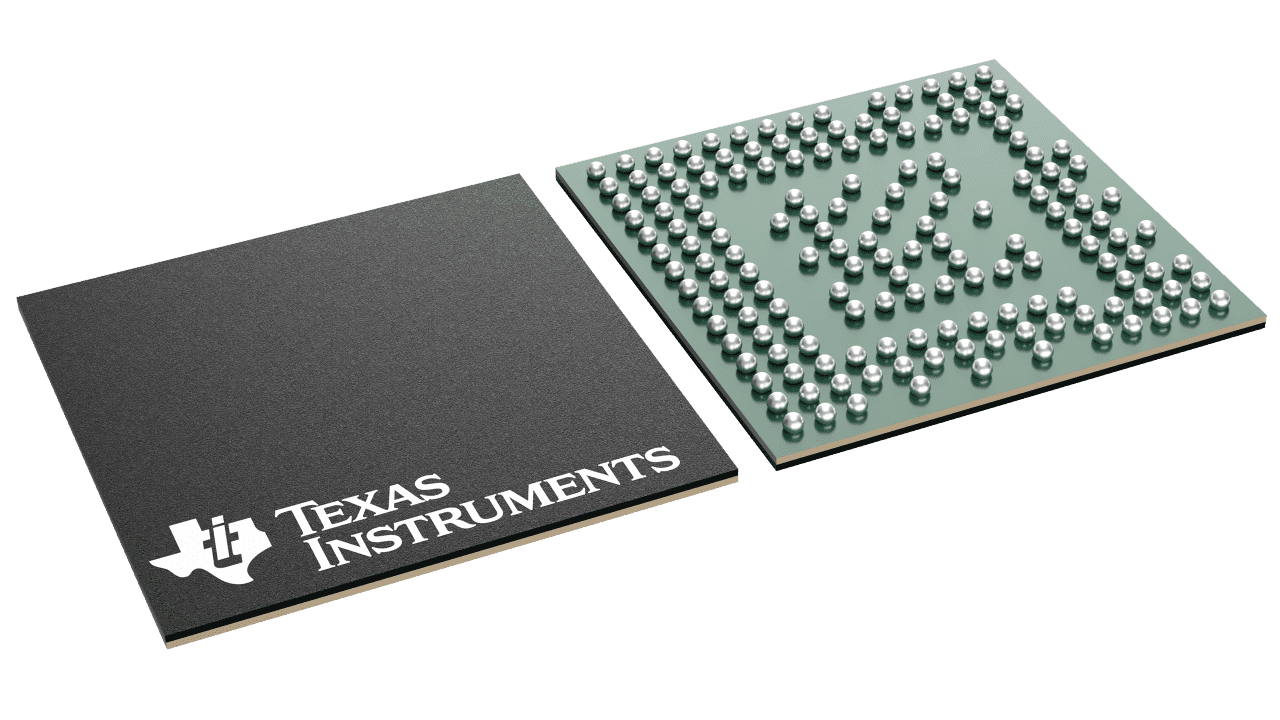
\includegraphics[width=0.5\textwidth]{AWR2243.png}
    \caption[Texas Instruments AWR2243 radar chip.]{Photo of the Texas Instruments AWR2243 radar chip, which is
    used in the radar module. The chip has 3 transmitters and 4 receivers, and outputs the radar data over a CSI
    video stream. The chip is only 10.4mm x 10.4mm, making it suitable for placement on UAV PCBs.}
    \label{fig:AWR2243}
\end{figure}

% \input{Sections/6 Practical Experience Logbook.tex}
\end{document}
